\documentclass[11pt]{article}

\usepackage[margin=1in]{geometry}
\usepackage{amsmath,amssymb}
\usepackage{booktabs}
\usepackage{colortbl}
\usepackage{array}
\usepackage{caption}
\usepackage{float}
\usepackage{tikz}
\usepackage{hyperref}
\usepackage[backend=biber,style=authoryear,natbib=true,maxcitenames=3,maxbibnames=20]{biblatex}
\setcounter{biburllcpenalty}{7000}
\setcounter{biburlucpenalty}{8000}
\setcounter{biburlnumpenalty}{7000}
\addbibresource{references.bib}
\usepackage{setspace}
\usepackage{xcolor}

\hypersetup{colorlinks=true,citecolor=blue!55!black,linkcolor=blue!55!black,urlcolor=blue!55!black}
\captionsetup{font=small,labelfont=bf}
\setlength{\parindent}{1.5em}
\setlength{\parskip}{0pt}
\onehalfspacing

\title{\textbf{Beyond the Status Quo, Beyond Stocks:\\Global Multi-Asset Portfolios and Lifecycle Investment Advice}}
\author{Guillaume Flament\\[2pt]
\normalsize Cayas\\[1pt]
\normalsize \href{mailto:guillaume.flament@cayas.fr}{guillaume.flament@cayas.fr}}
\date{August 28, 2026}

\begin{document}
\maketitle

\begin{abstract}
\noindent
\citet{AnarkulovaCederburgODoherty2025} find that lifecycle investors should
hold nothing but internationally diversified equities: a fixed 33/67 stock
portfolio, with no local bonds. We reproduce that ranking from fully public
data (the Jord{\`a}--Schularick--Taylor Macrohistory Database
\citep{MacrohistoryDB} for 16 developed markets, 1927--2025, in each household's
own currency and purchasing power) and extend the opportunity set to global
fixed income, gold, and a managed-futures sleeve. At 200\% gross
exposure, two pre-specified diversified families, whose weights and leverage
are chosen without reference to in-sample moments, match the all-equity
benchmark's 17.4\% annual
volatility but cut retirement ruin from 7.4\% to 1.8--2.5\%, and match its
lifecycle utility at a 5--6\% saving rate rather than 10\%. The ranking survives
risk aversion from 2 to 10 and varied contribution and withdrawal assumptions,
and weakens only beyond a sustained 200-basis-point financing spread. In this
extended historical design, diversification, not stock concentration, is favored
once the opportunity set is broad and strategies are compared at a common risk
budget rather than at a common gross exposure.

\medskip
\noindent \textit{JEL classifications:} C15, D14, G11, G17.\\
\noindent \textit{Keywords:} lifecycle asset allocation, international
diversification, leverage, gold, managed futures, retirement ruin.
\end{abstract}

\newpage

\section{Introduction}

Households saving for retirement face two related portfolio decisions. They
must choose which risks to hold and how much total risk to bear. Conventional
advice often combines the two: balanced and target-date portfolios add bonds
while reducing total market exposure. A large lifecycle literature embeds
these choices in models with labor income, longevity risk, and retirement
consumption \citep[e.g.,][]{CampbellViceira2002,CoccoGomesMaenhout2005}.

\citet{AnarkulovaCederburgODoherty2025}, hereafter ACO, challenge conventional
advice. In their broad international return panel and detailed lifecycle
model, the optimal fixed portfolio holds approximately 33\% domestic and 67\%
international equities, with no economically meaningful bond or bill
allocation. Internationally diversified equities also outperform conventional
balanced and target-date strategies in expected utility and capital
preservation. Their result is explicitly conditional on an opportunity set
containing domestic stocks, international stocks, local sovereign bonds, and
local bills.

This paper studies how far that ranking extends. ACO give the equity allocation
international breadth, but keep the \mbox{fixed-income} allocation local. A global
bond block can diversify sovereign, inflation, and currency histories that a
single local nominal bond cannot, and gold and managed futures add further
return mechanisms. \citet{BaiLiShen2024} extend this same pooled-bootstrap
lifecycle design toward housing and find that widening the opportunity set
beyond ACO's financial menu improves life-cycle outcomes. We widen it toward
diversified financial assets instead.

Broadening the opportunity set also separates two decisions that ACO's
all-equity rule ties together: which assets to hold, and how much total risk to
bear \citep{Markowitz1952,Asness1996}. A well-diversified portfolio has lower
standalone volatility, so it can be levered up to the equity risk budget while
keeping a higher risk-adjusted return. In frictionless markets that advantage
would be competed away---but many investors cannot or will not lever, and
instead bid up the most volatile assets directly, which sustains the advantage
\citep{FrazziniPedersen2014}. The composition of the levered portfolio is
therefore a real economic choice, not a neutral rescaling of the market.

Leverage, however, is only half of what the extension changes. The added
sleeves are measured in many currencies and deflated by many price indices,
which creates a measurement problem that is easy to miss in single-country or
dollar-based records: a real return is not a universal unit. A U.S.-dollar
return deflated by U.S. inflation
cannot be combined directly with a local return deflated by Australian,
German, or Japanese inflation. Every foreign asset must first be translated
into a single household's currency and then deflated by that household's price
index. Our panel performs this conversion separately for every country-year, so
each country-year row is an internally consistent real-return vector in one
currency and price index. ACO's bootstrap then chains such rows into a
simulated lifetime, and the numeraire follows the country each block is drawn
from (Section~\ref{sec:bootstrap}). Section~\ref{sec:usd-numeraire} holds the
same country-year states in a fixed dollar numeraire to show the importance of
that choice.

We first conduct a partial public-data replication of ACO on the full historical
panel. ACO estimate their result on proprietary monthly return data. We rebuild
the developed-market record from the Jord{\`a}--Schularick--Taylor Macrohistory
Database and public index and macro sources, so that both the replication and
the extensions can be checked and re-run by anyone. The fixed 33/67 portfolio
produces 7.36\% ruin, compared with 14.95\% for domestic stocks, 13.81\% for a
domestic 60/40, and 9.58\% for an internationally diversified balanced
portfolio. Domestic stocks require a 16.75\% saving rate to match the utility of
the 33/67 benchmark saving 10\%. These levels are not an exact replication of
ACO's monthly experiment, but the central ordering and economic magnitude are
similar. Reproducing either the ordering or the magnitudes alone could be a coincidence
of the panel. Reproducing both is what makes the replication credible and makes
it unlikely that the equity result is an artifact of the public panel.

Whether the later gold and managed-futures interactions would replicate on
ACO's proprietary data cannot be tested here, because both sleeves are
constructions rather than series an external dataset contains. The evidence
therefore splits into two layers. The covered-bond comparison and the currency
decomposition rely only on the Macrohistory series, the same sources that
reproduce the core ranking, and travel with it. The managed-futures and gold
results rest on these additional constructions and are the more
data-dependent layer.

We then decompose the equity result. A 33/67 portfolio at constant real
exchange rates produces 4.57\% ruin and matches benchmark utility with a
9.05\% saving rate. Restoring observed real-currency movements raises those
outcomes to 7.36\% and 10.00\%. Geographic diversification creates the gross
benefit, and historical currency exposure offsets part of it.

The central question is not whether a low-volatility multi-asset portfolio can
look safe, but whether diversification remains preferable once it uses the same
broad risk budget as ACO's all-equity rule. We hold the ACO 33/67 equity sleeve
fixed and evaluate two transparent four-sleeve families, made of equity, covered
world bonds, gold, and managed futures, at five pre-specified gross exposures
from 100\% to 200\%. No return mean, covariance, or volatility, in-sample or
rolling, selects their weights or leverage.

The answer in the full historical panel is affirmative. At the two 200\%
endpoints, the diversified families have annual volatility of 17.80\% and
17.02\%, bracketing ACO's 17.43\%, while retirement ruin is 1.83\% and 2.51\%
against 7.36\% for ACO. Their utility-equivalent saving rates are 5.32\% and
6.40\%, against 10\% for ACO. The central result is consequently stronger than
an isolated reduction in volatility. Within this extended opportunity set, the
100\% equity rule is not the best fixed portfolio rule at a comparable risk
budget. Diversification improves both capital preservation and lifecycle
utility.

This conclusion is deliberately scoped. A covered-bond sleeve by itself is
roughly on a par with all-equity, and the improvement comes from the joint
four-sleeve composition. The
pre-1968 gold price is the administered regime investors of the time actually
faced rather than a free-market record, and the numerical levels
depend on the resident-numeraire convention and stated financing terms. Currency
measurement nevertheless remains coherent throughout: every global asset is
converted into the resident's purchasing power before aggregation, and bond and
managed-futures returns are currency-hedged as the corresponding instruments
are.


\section{ACO and the Multi-Asset Extension}

\subsection{The benchmark result}
\label{sec:benchmark}

ACO simulate a U.S. couple that saves during a 40-year working life and draws
from financial wealth after retirement. Stochastic labor income, Social
Security, mortality, retirement consumption, and a bequest motive enter
expected utility. Their nonparametric block bootstrap resamples long sequences
of domestic stocks, international stocks, local government bonds, local bills,
inflation, and exchange rates from the pooled developed-market record. A single
simulated lifetime is a chain of multi-year blocks, and the country each block
is drawn from can differ from block to block: the pooled cross-section is the
distribution of return sequences a long-horizon household might draw
(Section~\ref{sec:methods-household}). Income, taxes, and preferences are
those of one U.S. couple throughout, and only the resampled asset-return and
inflation path varies.

The 2025 revision reports a fixed optimum of 33\% domestic and 67\%
international equities. It also explicitly permits leverage, and its own
comparative statics show the result depends on the financing spread. At their
lowest spread bonds can enter the optimum, and at higher spreads borrowing is
reduced or disappears. Our extension reproduces this spread dependence: its
levered rankings also weaken as the financing spread rises
(Section~\ref{sec:spread-sensitivity}). It asks whether broadening the assets
combined before leverage is chosen changes the ranking, and it prices borrowing
and hedging at what a household investing today can obtain rather than at a
historical rate.

There is an important asymmetry in this comparison. ACO obtain 33/67 by grid
searching the candidate weights that maximize average simulated utility, where
the bootstrap is calibrated from the full realized historical panel. It is thus
an in-sample selected optimum, not an allocation fixed without reference to the
realized return record. That is not literal look-ahead trading by the simulated
household, since a simulated return path is still drawn before its outcomes
occur. It is, however, an optimization-and-selection advantage for the
benchmark. Our
two diversified families are specified as simple weight rules and are not tuned
to estimated means, covariances, volatility, or their simulated utility,
although the choice of sleeves and family forms remains a model-selection
choice. A favorable comparison is consequently stronger than a comparison
between two portfolios each selected to maximize the same realized sample.
A natural worry is that 33/67 is an in-sample optimum only on ACO's
proprietary record. Re-running their grid search on our public panel, the
utility-maximizing equity mix lands at 30\% domestic and 70\% international,
with 33/67 within 0.02 points of equivalent saving of the grid's optimum.
The benchmark they selected is effectively the optimum of our data as well.

A second feature of the comparison matters as much. ACO rank portfolios by
expected lifecycle utility and let the CRRA curvature price risk on its own,
without holding the risk budget fixed across the portfolios compared. This is a
defensible modeling choice, but it makes the ranking sensitive to the level of
risk each rule happens to carry, and to the coefficient of relative risk
aversion. Their 33/67 rule runs at roughly 17\% annual volatility while the
domestic and balanced alternatives, all of which it beats, sit well below that
level, so part of the
gap is a difference in exposure rather than in composition. A cleaner question
is whether a diversified rule, scaled to the same risk budget as the all-equity
rule, still loses. Section~\ref{sec:leverage-ladders-main} shows it does not,
and Appendix~\ref{app:gamma-sensitivity} confirms that this holds for
coefficients of relative risk aversion from 2 to 10.

Because the proprietary monthly return data and private implementation code
are unavailable, our exercise is a partial replication. It omits ACO's
optimized age policy and target-date glidepath, and reproduces instead the
fixed domestic, 33/67, 50/50, balanced domestic, and balanced international
strategies under the published lifecycle preferences.

\subsection{Three empirical questions}

The analysis separates three questions.

First, does international equity diversification help before observed currency
movements are introduced? A constant-real-exchange-rate counterfactual keeps
the same markets and weights but neutralizes the joint nominal-exchange-rate
and inflation differential. An affirmative answer would confirm the principle
ACO have already established: the gain comes from spreading country risk.
Their convention could exhibit that principle only through equities, the most
volatile form diversification can take, and the remaining questions ask
whether lower-volatility assets carry the same geographic spread.
Second, does replacing a local fixed-income block with a broader
currency-hedged block
improve outcomes while keeping the equity sleeve, weights, and leverage fixed?
This is the same principle applied one sleeve down: spreading sovereign and
inflation risk across issuers rather than concentrating it in the resident's
own government. The relevant comparison
is the local 90/60 against a 90/60 whose bond sleeve becomes global while
financing remains in the resident currency.
The control changes both bonds and cash into unhedged foreign-currency
positions, and is deliberately not the main economic specification.

Third, once gold and managed futures complete a diversified fixed portfolio,
does that portfolio improve both capital preservation and expected utility over
ACO's 33/67 equity rule at a comparable risk budget? This is the question the
design builds toward. The first two questions spread risk inside a single asset
class, equities then sovereign debt. The third asks whether diversifying across
distinct return mechanisms genuinely improves both outcomes, or whether ACO's
equity-only answer already exhausted the gains.

None of these questions requires proprietary data. The public panel broadly
reproduces the same benchmark results ACO report, and the extension asks what
those results become once the opportunity set widens.


\section{Data}
\label{sec:data}

\subsection{Country-year panel and resident numeraire}

Every input to the lifecycle simulations is public. ACO estimate their result
on proprietary monthly return data. We rebuild the developed-market record from
open long-run sources, so the replication and every extension in this paper can
be reproduced from the cited series alone. The only proprietary series in the
paper are the SG and BarclayHedge managed-futures indexes, which appear solely
in the external comparison of Appendix~\ref{app:mf-external} and enter no
simulation. The panel begins with release~6 of the
Jord{\`a}--Schularick--Taylor Macrohistory Database
\citep{MacrohistoryDB,JordaEtAl2019}, which supplies nominal total returns on
equities and long-term government bonds, short rates, inflation, exchange rates, and
real GDP for 16 usable developed markets through 2020. We extend each series to
2025. Equity and bond total returns come from dividend-adjusted local index and
locally listed ETF data, and inflation and short rates from the Global Macro
Database \citep{MullerXuLehbibChen2025}, whose long-rate series coincides with
the Macrohistory one over the overlap. A source flag marks the appended years. On the 2006--2020 overlap the
reconstructed equity returns run about 1.2 points below the Macrohistory ones,
mostly ETF fees and large-cap indices, and the appended years are isolable for
any analysis that wants to drop them. The raw sample is an unbalanced panel of
1,557 country-years, which is also the main sample.

An ex ante investability
screen is retained as a labeled sensitivity. It excludes calendar years
overlapping the prolonged closures or restrictions reported for our countries
in ACO's Table~A.III and years with CPI inflation of at least 50\% or deflation
of at least 20\% in absolute value. These criteria identify observations for
which an annual vector cannot synchronize a tradable market, convertible
currency, and renewable hedge, and they do not depend on portfolio returns. The
raw rows are preserved in the replication package, and every calendar year from
1927 through 2025 remains represented.

Let $S_{c,f,t}$ denote units of resident currency $c$ per unit of foreign
currency $f$. If $R^{N}_{f,t}$ is a nominal foreign return and $\pi_{c,t}$ is
resident inflation, the resident-real return is
\begin{equation}
  1+R^{(c)}_{f,t}
  =(1+R^{N}_{f,t})
  \frac{S_{c,f,t}}{S_{c,f,t-1}}
  \frac{1}{1+\pi_{c,t}}.
  \label{eq:conversion}
\end{equation}
This spot conversion is applied to unhedged assets before portfolio
aggregation. It ensures that domestic equities, international equities, gold,
and the explicit unhedged controls on a country-year row all
measure the same change in household purchasing power.

International equity excludes the country of residence and uses lagged market
capitalization weights from the World Bank when
coverage is sufficient, with real-GDP weights (Maddison Project via the
Macrohistory Database, extended by \citealt{MullerXuLehbibChen2025}) as a
fallback. The 33/67 benchmark combines the resident's domestic market with this
foreign basket. The constant-real-exchange-rate counterfactual instead
aggregates each foreign market's local real return with identical weights. It
is an attribution device, not a hedged investment return, and it contains
neither forward carry nor hedging costs.

The world bond block equally weights every sovereign in the panel that has a
usable bond, bill, and exchange rate in a given year. It holds 16 issuers in
1,312 of 1,557 country-years and never fewer than 12. Years with fewer than
eight available issuers are dropped, which costs no observation after 1927. The
block includes the resident's own sovereign, as an actual global bond index
does, so the basket is common to all residents in a year and covered interest
parity applies to it directly. Each bond is currency-hedged under that parity,
so its excess return over its own bill is combined with the resident bill.
Financing is therefore always local. We subtract ten basis points annually from
covered notionals in the baseline. The unhedged foreign bond and bill basket is
retained only as a labeled diagnostic control. The resulting block is wider
than a four-issuer basket but still covers developed markets only, so it is not
exhaustive global fixed income.

\subsection{Gold and managed futures}

Gold uses the annual U.S.-dollar price compiled by MeasuringWorth
\citep{OfficerWilliamsonMeasuringWorth} through 1967 and the LBMA afternoon
fixing \citep{LBMA} from 1968, the first year a free market existed. Both are
dollars per troy ounce and are spliced without recalibration. We subtract 40
basis points per year for custody, convert the resulting U.S.-dollar return
into each resident currency, and deflate by resident inflation. The dollar
price was administered for much of the first 41 years and private U.S.
ownership and convertibility were restricted. Nor is this a U.S. peculiarity:
under the gold standard and the Bretton Woods pegs, every panel currency's
gold price was administered through its parity, so the low-variance segment
is a property of the era for all residents rather than of the U.S. series
alone. Those
observations are coherent with what a contemporaneous investor could actually
hold, but their low
dollar-price variance is not an investable free-market estimate of prospective
gold risk. We therefore treat gold results as sensitivity evidence rather than
a structural estimate \citep{ErbHarvey2013}. Appendix~\ref{app:gold-availability}
also reports an availability rule under which, before 1968, the gold notional is
allocated equally across the non-gold sleeves already present in the portfolio.

No free investable managed-futures index spans the sample, so we reconstruct a
monthly time-series-momentum proxy. The design follows a well-established
literature. \citet{MoskowitzOoiPedersen2012} document that the sign of an
asset's own past twelve-month return predicts its next-month return across
roughly 58 futures markets, and that scaling each position by inverse
volatility and averaging produces a diversified premium. \citet{HurstOoiPedersen2017}
extend the same rule back to 1880 and show that a blend of one-, three-, and
twelve-month look-backs is stable across a century of data and across asset
classes. \citet{BaltasKosowski2020} study the construction choices themselves,
finding that the signal horizon, the rebalancing frequency, and the resulting
turnover jointly determine net performance and capacity, which motivates our
one-, six-, and twelve-month blend and the explicit turnover cost below.
\citet{LempiereEtAl2014} find a trend premium in equities, bonds, currencies,
and commodities as far back as 1800, which is what justifies applying the rule to
the full 1927--2025 window. Trend following also lowers sequence risk in
retirement decumulation \citep{ClareSeatonSmithThomas2017,ClareSeatonSmithThomas2019}
and improves risk-parity implementations through correlation-aware weighting
\citep{Baltas2015}. That literature, however, stops at portfolio-level
backtests: none of it embeds trend following in a full lifecycle model with
the pooled developed-market panel, which is the gap the lifecycle results of
Section~\ref{sec:leverage-ladders-main} fill.

The word ``monthly'' refers solely to the construction of this sleeve. It
does \emph{not} mean that we interpolate the annual JST/Macrohistory panel
used for domestic equity, bonds, bills, inflation, and the bootstrap. The MF
signal instead reads a separate, frozen monthly price snapshot, and only its
completed calendar-year returns are then joined to the annual household panel.
Appendix~\ref{app:mf-monthly-data} documents that snapshot, its sources, and
the monthly-to-annual transformation in detail.

In our implementation, signals average the signs of prior one-, six-, and
twelve-month returns. Volatility uses the preceding 36 months, and the aggregate
strategy targets 10\% volatility with a three-times scalar cap. The universe
expands across four sectors as data become available: 18 national price indexes
and 18 synthetic ten-year sovereign positions, 19 commodities plus gold and
silver, and six dollar foreign-exchange forwards. The monthly equity and yield
inputs come principally from the OECD Main Economic Indicators via FRED
\citep{OECDMEI,FRED}, with the early U.S., U.K., German, French, commodity, and
rate segments supplied by the monthly NBER Macrohistory files
\citep{NBERMacrohistory}. Commodities are extended with the World Bank ``Pink
Sheet'' \citep{WorldBankPinkSheet}, and currencies use month-end Federal
Reserve H.10 quotations \citep{FedH10}. Where two sources meet, the return
that straddles the junction is left missing rather than computed from spliced
price levels, which would fabricate an artificial price change. Sector Sharpe ratios over
the full reconstruction are 0.44 (equities), 0.50 (rates), 0.47 (currencies),
and 0.36 (commodities), against 0.41, 0.49, 0.57, and 0.80, respectively, in the
Capital Fund Management estimates of \citet{LempiereEtAl2014}, and the combined
figure is 0.77 against 0.80.

The proxy carries a separate monthly U.S.-dollar cash-collateral return from
that snapshot. We remove this exact embedded collateral and combine the
remaining excess return with the resident bill, so the main series is
currency-hedged with carry. This avoids substituting an approximate annual bill
series for the cash actually earned by the proxy.
We subtract a 0.85\% annual management
fee and transaction costs based on measured turnover of 18.88 times per year
and a three-basis-point spread, or 0.57\% annually. Its monthly correlation with
several official CTA indexes is 0.49--0.53 over 2000--2025.

\subsection{Realized portfolio properties}

Table~\ref{tab:moments} reports pooled country-year moments. These are
descriptive outcomes of the fixed portfolios above, not inputs to their design.
The final column is the 1\% annual-return quantile, not a maximum drawdown and
not the raw minimum. The covered global-bond test displays the expected diversification
pattern, with volatility of 16.83\% against 17.44\% for the otherwise identical
local 90/60. The full panel, including Japan 1945 and other disrupted markets,
is the reported historical distribution, and the investability screen is a
separate sensitivity.

\begin{table}[t]
\centering
\caption{Realized resident-real portfolio properties}
\label{tab:moments}
\begin{tabular}{lrrr}
\toprule
Portfolio & Mean return & Volatility & 1\% annual return \\
\midrule
Domestic stocks & 7.65\% & 23.32\% & $-45.20\%$ \\
ACO 33/67, constant real FX & 7.47 & 15.75 & $-37.42$ \\
ACO 33/67 & 7.58 & 17.43 & $-39.42$ \\
Balanced domestic & 5.45 & 15.76 & $-31.59$ \\
Balanced/I & 5.42 & 12.71 & $-27.46$ \\
90/60 local, fixed & 7.79 & 17.44 & $-35.45$ \\
90/60 global bonds, covered & 7.69 & 16.83 & $-34.88$ \\
60/40 ACO/covered & 5.33 & 11.94 & $-25.60$ \\
60/40 ACO $+$ 33.33 MF & 7.19 & 13.05 & $-21.37$ \\
60/40 ACO $+$ 33.33 gold & 6.21 & 13.68 & $-22.40$ \\
54/36/20/20 ACO & 6.50 & 12.28 & $-19.12$ \\
90/60/25/25 ACO & 9.74 & 18.34 & $-28.90$ \\
\bottomrule
\end{tabular}
\begin{minipage}{0.94\textwidth}\footnotesize
\textit{Note:} Arithmetic means, standard deviations, and the linearly
interpolated 1\% quantile of pooled one-year returns across all 1,557
country-years. The final column is the annual return at which 1\% of the
country-year observations are lower. It is a left-tail return measure, not a
probability of ruin, a maximum drawdown, or the single worst historical year.
This is the volatility of the annual return series itself, not
the volatility of a simulated retirement path (which Table~\ref{tab:frontier}
reports and which is lower because bootstrap blocks average). Every return is
expressed in the currency and purchasing power of the household associated with
that row. Bonds and MF are currency-hedged in the main portfolios, equity and
gold are not. MF denotes reconstructed managed futures net of baseline fees and
transaction costs.
\end{minipage}
\end{table}


\section{Lifecycle Model and Portfolio Design}

\subsection{Household, income, and retirement}
\label{sec:methods-household}

The household is a couple aged 25. Each spouse receives an independent
stochastic earnings history through age 64 based on model 6 of
\citet{GuvenenKarahanOzkanSong2021}. Log income contains a quadratic age
profile, a persistent component with autoregressive coefficient 0.959,
transitory shocks, and age- and income-dependent nonemployment. The household
saves a constant fraction of each spouse's income when that individual's
annual income is at least \$15,000. Contributions occur at the beginning of
the year and then receive the annual portfolio return.

At age 65 the couple fixes a real annual withdrawal equal to 4\% of retirement
wealth, following \citet{Bengen1994} and ACO. A fixed real withdrawal makes the
retirement outcome sensitive to the order in which returns arrive, not only to
their average: a sequence of early losses can exhaust the account even when
long-run returns are adequate, and international evidence shows the safe rate
varies widely across historical return paths \citep{Estrada2018}.
Appendix~\ref{app:policy-sensitivity} varies the withdrawal rate from 3\% to
5\% and the contribution rate from 5\% to 15\% and finds the diversified
ranking unchanged. Social
Security is calculated from each simulated earnings history using 2022 bend
points, spouse and survivor benefits, and the early-claiming adjustments
described by ACO. Supplemental Security Income supplies a consumption floor.
Ruin occurs when financial wealth cannot fund the fixed withdrawal before the
last spouse dies. Public pension income continues after financial wealth is
exhausted.

Mortality follows sex-specific Gompertz--Makeham laws calibrated to the joint
retirement and longevity moments reported by ACO from Social Security
Administration tables \citep{SSA2020}. Return paths, income histories, and
death draws are paired across strategies.

This household is hybrid by construction, exactly as in ACO. Earnings, Social
Security, Supplemental Security Income, and preferences are U.S., while the
return-and-inflation path it earns is resampled from the pooled
developed-market panel and can move across countries and numeraires from one
block to the next. A simulated life is therefore a distributional statement,
not a description of any actual investor's experience: the saver keeps the
American earnings process, retirement institutions, and preferences, while the
macro history it lives through, down to the currency and price index of each
decade, is drawn from the recorded
histories of sixteen developed markets. The underlying view is that a single
U.S. history is one draw from that set, too thin to characterize its tails.
The cost of the
assumption is that a lifetime can splice, say, a high-inflation
1970s decade in one country onto a deflationary decade in another. The benefit
is an order of magnitude more independent return-and-inflation history, about
1{,}500 country-years against roughly a
century. We keep ACO's choice here so that our extensions are measured against
their benchmark on the same terms, and Section~\ref{sec:bootstrap} gives the
mechanics.

\subsection{Utility and equivalent saving}

For annual real consumption $C_t$, household size $H_t$, bequest $B$, and last
year alive $T$, utility is
\begin{equation}
 U(C,B)=\sum_{t=65}^{T}
 \frac{(C_t/\sqrt{H_t})^{1-\gamma}}{1-\gamma}
 +\theta\frac{(B+k)^{1-\gamma}}{1-\gamma}.
 \label{eq:utility}
\end{equation}
Risk aversion is $\gamma$ = 3.84, and the bequest motive has intensity
$\theta$ = 2,360 with shifter $k$ = \$490,000. None of the three is our
choice. They are the estimates of \citet{DeNardiFrenchJones2010}, fitted to
retiree data in a lifecycle model with medical expenses, and ACO adopt them
unchanged, so our benchmark utility is exactly theirs. The bequest term is
additive and warm-glow: utility depends on the size of the estate left,
$B+k$, not on the heirs' own circumstances, which is the specification that
explains why retirees in the data run down wealth slowly. ACO evaluate monthly
consumption and therefore multiply the annual bequest-intensity estimate by
$12^\gamma$. If within-year consumption is uniform, dividing their
entire monthly utility by $12^\gamma$ gives equation~\eqref{eq:utility} with
$\theta$ = 2,360. The annual aggregation thus preserves the relative scale of
consumption and bequest utility, and only the wealth dynamics remain an annual
approximation.

For strategy $j$, the equivalent saving rate $s_j^*$ solves
\begin{equation}
 E[U_j\mid s_j^*]
 =E[U_{33/67}\mid s=0.10].
 \label{eq:eqsaving}
\end{equation}
A rate below 10\% means that the strategy attains benchmark utility with less
saving. All other reported wealth, consumption, ruin, and bequest outcomes use
the common 10\% saving rate, not $s_j^*$.
This is a welfare comparison of the complete portfolio choice, including its
total risk. It is not a risk-normalized performance measure, since a
lower-volatility portfolio can rationally have a higher equivalent saving rate
while offering a different risk budget. To isolate composition from total
exposure, Appendix~\ref{app:leverage-ladders} reports pre-specified
gross-exposure ladders and compares only portfolios in a common
realized-volatility band. The band is a descriptive presentation device, and
the weights themselves are not calibrated to volatility.

\subsection{Fixed, non-estimated portfolio rules}
\label{sec:portfolio-rules}

Table~\ref{tab:design} defines the main extensions. The 90/60 local strategy
holds 90\% in the ACO 33/67 equity portfolio and 60\% in the residence-country
sovereign bond, financed with a 50\% short local-bill position plus the
financing spread $\phi$ on the borrowed portion. The intermediate
strategy changes only the bond sleeve to the covered global aggregate, with
financing still in the resident bill. Every other extension also uses the
same 33/67 resident equity return. The designs therefore vary fixed income,
alternative sleeves, and total exposure without changing equity geography.

\begin{table}[t]
\centering
\caption{Fixed portfolio rules}
\label{tab:design}
\begin{tabular}{lrrrrrr}
\toprule
Portfolio & Equity & Bonds & Gold & MF & Sleeve sum & Financing \\
\midrule
ACO 33/67 & 100\%$^{a}$ & 0\% & 0\% & 0\% & 100\% & 0\% \\
90/60 local & 90$^{a}$ & 60$^{b}$ & 0 & 0 & 150 & 50 \\
90/60 global bonds, covered & 90$^{a}$ & 60$^{c}$ & 0 & 0 & 150 & 50 \\
60/40 ACO/covered & 60$^{a}$ & 40$^{c}$ & 0 & 0 & 100 & 0 \\
60/40 ACO $+$ 33.33 MF & 60$^{a}$ & 40$^{c}$ & 0 & 33.33 & 133.33 & 33.33 \\
60/40 ACO $+$ 33.33 gold & 60$^{a}$ & 40$^{c}$ & 33.33 & 0 & 133.33 & 33.33 \\
54/36/20/20 ACO & 54$^{a}$ & 36$^{c}$ & 20 & 20 & 130 & 30 \\
90/60/25/25 ACO & 90$^{a}$ & 60$^{c}$ & 25 & 25 & 200 & 100 \\
\bottomrule
\end{tabular}
\begin{minipage}{0.97\textwidth}\footnotesize
\textit{Note:} Percentages of investor capital. $^{a}$33\% domestic and 67\%
international equities. $^{b}$Residence-country government bond and bill.
$^{c}$Currency-hedged equal-weight global sovereign bonds with resident-currency
financing. The equity sleeve remains 33/67.
``Sleeve sum'' is the sum of index-level allocations,
and financing is the corresponding external cash financing in the return
equation.
\end{minipage}
\end{table}

The weights are design inputs, fixed before any evaluation. That discipline
eliminates a direct full-sample leverage
calibration, but it is not a pre-registration and does not eliminate
strategy-family selection.

The manifest also contains two fixed leverage ladders, each stepping a
four-sleeve family through 100, 125, 150, 175, and 200\% gross exposure: one
proportional to 60/40/25/25 (equity/covered bonds/gold/managed futures), the
other equal-weight across the four sleeves. The levels are fixed before
evaluation and target no realized volatility. These ladders carry the central
comparison in Section~\ref{sec:leverage-ladders-main}.

For a foreign bond with local-real return $R^f_{b,t}$ and foreign bill
$R^f_{f,t}$, covered interest parity gives the resident-real covered return
\begin{equation}
  1+R^{c,H}_{b,t}
  =(1+R^c_{f,t})\frac{1+R^f_{b,t}}{1+R^f_{f,t}}.
  \label{eq:covered}
\end{equation}
This preserves the foreign term premium while replacing foreign cash with the
resident bill. Let every $R^{(c)}_{i,t}$ then be in the common resident-real
numeraire. A portfolio whose index-level sleeve sum is $G_j$ has return
\begin{equation}
 R^{(c)}_{j,t}=\sum_i w_i R^{(c)}_{i,t}
 +(1-G_j)R^{(c)}_{f,t}
 -\max(G_j-1,0)\phi-h_j\kappa,
 \label{eq:return}
\end{equation}
where $\phi$ is the financing spread, $h_j$ is covered notional, and $\kappa$
is the hedge friction. Managed futures already include the U.S. cash return
observed in their source series. Replacing that exact collateral return with the
resident bill, while retaining the negative financing position, prevents cash
yield from being omitted or counted twice.

For a levered portfolio ($G_j>1$), the coefficient on the resident bill in
equation~\eqref{eq:return} is negative. Holding all asset returns fixed, a
higher ex-post real bill therefore lowers the portfolio return, while an
inflation surprise that lowers the ex-post real bill raises it. This is an
accounting implication of the annual return convention, not a claim about the
timing or availability of short-term borrowing within the year.

The baseline values, $\phi = 30$ and $\kappa = 10$ basis points, are meant as
the cost a household investing today would face, not the cost a household in the
1930s or 1970s would have faced. A retail investor now obtains embedded leverage
close to $\phi$ through a levered or return-stacked ETF, or finances a long
position directly at an implied rate a few tens of basis points over Treasury
bills using an exchange-traded box spread. Hedging a developed-market bond
sleeve with forward currency contracts trades at a similar order of magnitude.
The fixed sleeve weights and 200\% gross-exposure cap of the ladders in
Section~\ref{sec:leverage-ladders-main} can be held today with a small number of
packaged funds: broad equity, return-stacked bond and managed-futures, and gold
ETFs. Each fund manages its own leverage continuously to a target exposure, so
the household holds no margin position of its own and faces no personal margin
call on the levered sleeve. Forced deleveraging in a drawdown happens inside the
fund, not in the investor's account. The household's only rebalancing is across
these funds, back to the fixed sleeve weights, which the annual return
convention of the model matches and which a real investor can do infrequently.
Carrying the same leverage on a personal margin account, where a deep drawdown
can trigger a call, is a do-it-yourself alternative, not the implementation the
cost assumptions describe. Appendix~\ref{app:margin-call} shows that these
same levered books, carried on such an account with the same annual
rebalancing, never breach a 25\% maintenance margin at annual granularity on
the pooled panel. Applying
that present-day cost to the whole 1927--2025 return distribution is
deliberate. What counts is what an investor today knows and can set up: the
historical record enters as evidence about the paths asset markets can take,
while borrowing and hedging are implemented on today's terms. It is not a
claim that such terms existed throughout the sample. Where they plainly did
not (under capital controls,
closed futures markets, or wartime financing), the observations nevertheless
remain in the raw central panel. The investability screen of
Section~\ref{sec:data} is reported only as a sensitivity. Because the choice of
$\phi$ is a modeling input rather than an estimate,
Section~\ref{sec:spread-sensitivity} re-runs the levered comparisons
at $\phi = 60$ and 100 basis points.

\subsection{Bootstrap and inference}
\label{sec:bootstrap}

The main fixed-portfolio experiment draws 10,000 paths using a stationary block
bootstrap with mean block length ten years, following ACO. Long blocks are
deliberate: they preserve the horizon-dependent risk of equities, such as the
long-run mean reversion documented by \citet{PoterbaSummers1988}, and the
persistence of real interest rates, both of which an i.i.d.\ resample of annual
returns would destroy. Within a block the country is fixed: the block advances
year by year through one country's history and retains that country-year's
joint observation of domestic equity, the international basket, the global bond
and bill blocks, gold, managed futures, inflation, and the exchange rate. A new origin is drawn from the pooled panel
when the block ends or the country's series has a gap, and that origin can fall
in a different country, so a simulated lifetime is a sequence of country-decades
rather than a single national history. This is ACO's resampling scheme
unchanged. Section~\ref{sec:methods-household} discusses its interpretation.

Our resident-numeraire conversion operates inside each block. Because every
asset on a country-year row is already expressed in that country's currency and
price index (Section~\ref{sec:data}), a block drawn from, say, Japan in the
1980s is a fully consistent yen-real decade, with domestic and foreign equity,
the hedged bond and managed-futures blocks, and inflation all measured in one
household's purchasing power, and the numeraire changes only when the next
block is drawn from another country. This is one coherent way to define the
pooled distribution, not the only valid one. A fixed-numeraire construction
instead converts every source state into that numeraire. We implement the
fixed-dollar version in Section~\ref{sec:usd-numeraire}. Both remain
synthetic, for the reason Section~\ref{sec:methods-household} gives.

We report normal 95\% intervals for the paired difference in ruin relative to
the 33/67 benchmark. These intervals measure Monte Carlo uncertainty
conditional on the observed panel. They do not treat 1,557 country-years as
independent observations. Appendix~\ref{app:historical-uncertainty} separately
perturbs the historical sample itself, and its ranges are sensitivity
diagnostics, not confidence intervals.


\section{Results}

\subsection{Partial replication and equity attribution}

Table~\ref{tab:currency} presents the public-data replication and attribution.
The lifecycle model reproduces ACO's central ordering. The 33/67 benchmark
substantially lowers the retirement-ruin probability of a domestic all-equity
portfolio, from 14.95\% to 7.36\%, and a domestic household must save close to
17\% of income to match its utility. Both balanced portfolios are worse in
utility, and even the internationally diversified one does not preserve capital
better than 33/67. The public annual panel therefore recovers the same
domestic-to-international improvement that motivates ACO's conclusion. The
replicated lifecycle model is thus close enough to theirs to support the
extensions. The constant-real-exchange-rate row attributes this
domestic-to-international gain, and ruin tells the story most simply. Domestic
stocks start at 14.95\%. Holding real currency movements fixed while broadening
the equity opportunity set cuts ruin to 4.57\%, so pure geographic breadth
removes 10.38 points. Restoring observed currency movements adds 2.79 points
back and lands on the published 7.36\%, a net improvement of 7.59 points. The
equivalent saving rate decomposes the same way: breadth lowers it by 7.70
points, the currency channel adds back 0.95 point, and the net improvement is
6.75 points. Breadth thus accounts
for more than the whole net improvement, and the currency channel offsets part
of it rather than adding to it. The constant-FX row is an attribution device, not an
implementable portfolio, and does not imply that hedging equity currency would
reproduce it. It is nonetheless the first sign of the principle the paper tests
throughout: diversification itself pays.
\begin{table}[t]
\centering
\caption{Public-data replication and equity attribution}
\label{tab:currency}
\begin{tabular}{lrrr}
\toprule
Portfolio & Utility-eq. saving & Ruin & Median wealth at 65 \\
\midrule
Domestic stocks & 16.75\% & 14.95\% & \$742,494 \\
ACO 33/67, constant real FX & 9.05 & 4.57 & 889,583 \\
ACO 33/67 & 10.00 & 7.36 & 904,948 \\
Stocks/I 50/50 & 10.41 & 8.06 & 883,084 \\
Balanced domestic & 18.53 & 13.81 & 589,241 \\
Balanced/I & 14.79 & 9.58 & 629,208 \\
\bottomrule
\end{tabular}
\begin{minipage}{0.94\textwidth}\footnotesize
\textit{Note:} 10,000 paired simulations. Utility-equivalent saving matches
expected lifecycle utility, not wealth, relative to ACO 33/67 at 10\%.
Constant real FX neutralizes the joint nominal-currency and
relative-inflation movement without forward carry or hedging costs.
\end{minipage}
\end{table}

\subsection{Diversification improves on ACO at a comparable risk budget}
\label{sec:leverage-ladders-main}

The fixed recipes in Table~\ref{tab:lifecycle} are useful accounting benchmarks,
but their different volatility makes them a poor centerpiece for the economic
comparison. The demanding test uses the two four-sleeve ladders defined in
Section~\ref{sec:portfolio-rules}, stepped through 100 to 200\% gross exposure
at the pre-specified levels. The comparison is
asymmetric by design: the 33/67 rule is an in-sample utility maximum, while the
ladder rows follow the simple rules of Section~\ref{sec:benchmark}. The design also keeps the ACO 33/67
equity sleeve throughout, so diversification is not obtained by changing the
benchmark equity portfolio. The 90/60 local and covered-bond rows
in Table~\ref{tab:lifecycle} are a check: global covered bonds improve the local
90/60 (ruin 7.81\% versus 8.52\%) but alone do not beat ACO's 7.36\%, so the
result below requires the joint four-sleeve composition.
Diversifying the local bond sleeve into currency-hedged global bonds genuinely
improves the outcome, but the levered covered 90/60 is effectively
tied with 100\% equity at the baseline spread and edges past it
only when the financing spread falls to zero (Table~\ref{tab:spread}). The
window matters as much as the spread: on 1970--2025 the same levered covered
90/60 improves on both criteria, with ruin of 2.91\% against ACO's 4.22\% and
equivalent saving of 8.28\% against 10\%, while over the full panel it is
effectively tied. Levering
bonds borrows at the resident bill to hold assets whose expected excess over
that bill is a thin term premium on the full panel, so the levered position
mostly amplifies risk
the equity block already dominates, and the financing drag absorbs much of the
difference. The 1970--2025 result shows the balance is regime-dependent rather
than structural. The design lesson for the evidence base we use is unchanged:
bonds do carry a return source of their own, the term premium, but it is thin
per unit of added risk and thinner still after financing costs. A sleeve that
beats all-equity robustly must bring an incremental premium large enough to
survive that drag, which is what gold and managed
futures contribute below.

\begin{table}[t]
\centering
\caption{Lifecycle outcomes of fixed portfolios}
\label{tab:lifecycle}
\setlength{\tabcolsep}{2.8pt}
\small
\begin{tabular}{lrrrrr}
\toprule
Portfolio & Utility-eq. rate & Wealth at 65 & Mean consumption & Ruin & Median bequest \\
\midrule
ACO 33/67 & 10.00\% & \$904,948 & \$73,166 & 7.36\% & \$1,532,124 \\
90/60 local & 9.91 & 958,531 & 77,334 & 8.52 & 1,769,958 \\
90/60 global bonds, covered & 9.77 & 950,885 & 76,286 & 7.81 & 1,745,595 \\
60/40 ACO/covered & 14.41 & 629,380 & 55,870 & 8.90 & 687,604 \\
60/40 ACO $+$ 33.33 MF & 8.70 & 921,663 & 71,271 & 3.29 & 1,770,421 \\
60/40 ACO $+$ 33.33 gold & 11.00 & 733,983 & 61,136 & 4.38 & 1,071,052 \\
54/36/20/20 ACO & 9.76 & 807,938 & 63,758 & 3.19 & 1,347,002 \\
90/60/25/25 ACO & 5.36 & 1,465,946 & 103,355 & 1.96 & 4,905,367 \\
\bottomrule
\end{tabular}
\begin{minipage}{0.98\textwidth}\footnotesize
\textit{Note:} 10,000 paired simulations, baseline spread 0.30\% and hedge friction 0.10\%.
All wealth, consumption, ruin, and bequest columns use 10\% saving.
\mbox{Utility-equivalent} saving alone varies the contribution rate to match expected ACO
33/67 lifecycle utility, and does not target equal retirement wealth.
\end{minipage}
\end{table}

\begin{table}[t]
\centering
\caption{Two pre-specified diversified leverage ladders}
\label{tab:main-ladders}
\setlength{\tabcolsep}{3pt}
\small
\begin{tabular}{llrrr}
\toprule
Family & Gross exposure & Volatility & Saving & Ruin \\
\midrule
60/40/25/25 proportional & 100\% & 10.00\% & 13.17\% & 4.87\% \\
 & 125\% & 11.82 & 10.25 & 3.32 \\
 & 150\% & 13.75 & 8.13 & 2.47 \\
 & 175\% & 15.75 & 6.54 & 2.06 \\
 & 200\% & 17.80 & 5.32 & 1.83 \\
\addlinespace
Equal-weight four-sleeve & 100\% & 9.68 & 14.54 & 5.79 \\
 & 125\% & 11.38 & 11.57 & 4.10 \\
 & 150\% & 13.19 & 9.36 & 3.27 \\
 & 175\% & 15.08 & 7.70 & 2.64 \\
 & 200\% & 17.02 & 6.40 & 2.51 \\
\bottomrule
\end{tabular}
\begin{minipage}{0.95\textwidth}\footnotesize
\textit{Note:} 10,000 paired simulations on the 1{,}557-country-year raw
panel. ``Volatility'' is the pooled annual standard deviation. The equity sleeve
is ACO 33/67, and bonds and managed futures are covered. The five gross-exposure
levels and both family definitions are fixed before evaluation.
\end{minipage}
\end{table}

\begin{figure}[t]
\centering
% Généré par build/plot_ladders_main.py — ne pas éditer à la main.
% Source : results/main_ladders_n10000.json (seed 20260827, 10000 traj.).
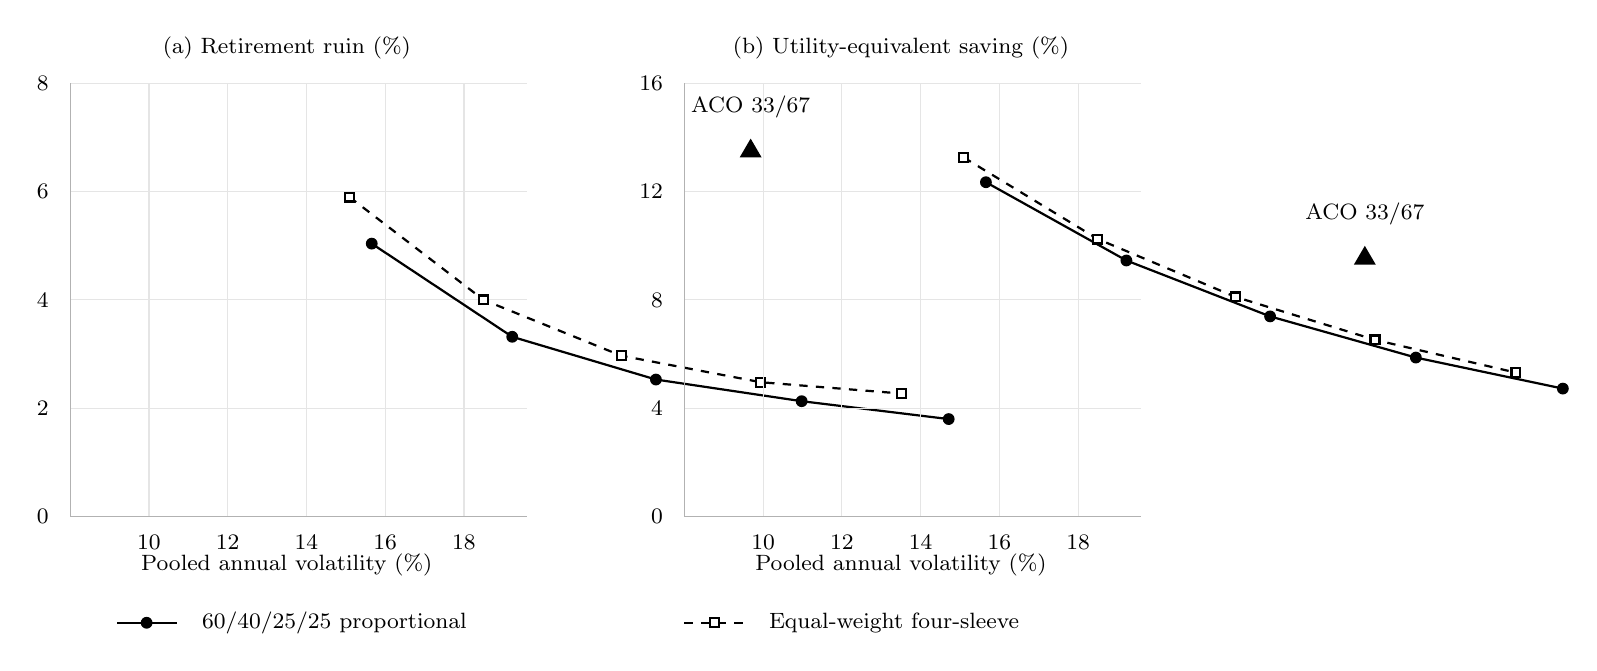
\begin{tikzpicture}[x=1cm, y=1cm]
\begin{scope}[shift={(0.0,0)}]
  \draw[gray!20] (0,0.000) -- (5.80,0.000);
  \node[left, font=\footnotesize] at (-0.15,0.000) {0};
  \draw[gray!20] (0,1.375) -- (5.80,1.375);
  \node[left, font=\footnotesize] at (-0.15,1.375) {2};
  \draw[gray!20] (0,2.750) -- (5.80,2.750);
  \node[left, font=\footnotesize] at (-0.15,2.750) {4};
  \draw[gray!20] (0,4.125) -- (5.80,4.125);
  \node[left, font=\footnotesize] at (-0.15,4.125) {6};
  \draw[gray!20] (0,5.500) -- (5.80,5.500);
  \node[left, font=\footnotesize] at (-0.15,5.500) {8};
  \draw[gray!20] (1.000,0) -- (1.000,5.500);
  \node[below, font=\footnotesize] at (1.000,-0.12) {10};
  \draw[gray!20] (2.000,0) -- (2.000,5.500);
  \node[below, font=\footnotesize] at (2.000,-0.12) {12};
  \draw[gray!20] (3.000,0) -- (3.000,5.500);
  \node[below, font=\footnotesize] at (3.000,-0.12) {14};
  \draw[gray!20] (4.000,0) -- (4.000,5.500);
  \node[below, font=\footnotesize] at (4.000,-0.12) {16};
  \draw[gray!20] (5.000,0) -- (5.000,5.500);
  \node[below, font=\footnotesize] at (5.000,-0.12) {18};
  \draw[gray!60] (0,0) -- (5.80,0);
  \draw[gray!60] (0,0) -- (0,5.500);
  \fill (8.641,4.799) -- ++(-0.14,-0.24) -- ++(0.28,0) -- cycle;
  \node[font=\footnotesize, anchor=south] at (8.641,4.939) {ACO 33/67};
  \draw[thick] plot coordinates {(3.829,3.465) (5.613,2.282) (7.438,1.739) (9.289,1.464) (11.156,1.237)};
  \fill (3.829,3.465) circle (0.075);
  \fill (5.613,2.282) circle (0.075);
  \fill (7.438,1.739) circle (0.075);
  \fill (9.289,1.464) circle (0.075);
  \fill (11.156,1.237) circle (0.075);
  \draw[thick, dashed] plot coordinates {(3.547,4.056) (5.250,2.750) (6.997,2.042) (8.770,1.705) (10.560,1.561)};
  \node[draw, thick, rectangle, inner sep=1.6pt, fill=white] at (3.547,4.056) {};
  \node[draw, thick, rectangle, inner sep=1.6pt, fill=white] at (5.250,2.750) {};
  \node[draw, thick, rectangle, inner sep=1.6pt, fill=white] at (6.997,2.042) {};
  \node[draw, thick, rectangle, inner sep=1.6pt, fill=white] at (8.770,1.705) {};
  \node[draw, thick, rectangle, inner sep=1.6pt, fill=white] at (10.560,1.561) {};
  \node[font=\footnotesize] at (2.75,5.95) {(a) Retirement ruin (\%)};
  \node[font=\footnotesize] at (2.75,-0.62) {Pooled annual volatility (\%)};
\end{scope}
\begin{scope}[shift={(7.8,0)}]
  \draw[gray!20] (0,0.000) -- (5.80,0.000);
  \node[left, font=\footnotesize] at (-0.15,0.000) {0};
  \draw[gray!20] (0,1.375) -- (5.80,1.375);
  \node[left, font=\footnotesize] at (-0.15,1.375) {4};
  \draw[gray!20] (0,2.750) -- (5.80,2.750);
  \node[left, font=\footnotesize] at (-0.15,2.750) {8};
  \draw[gray!20] (0,4.125) -- (5.80,4.125);
  \node[left, font=\footnotesize] at (-0.15,4.125) {12};
  \draw[gray!20] (0,5.500) -- (5.80,5.500);
  \node[left, font=\footnotesize] at (-0.15,5.500) {16};
  \draw[gray!20] (1.000,0) -- (1.000,5.500);
  \node[below, font=\footnotesize] at (1.000,-0.12) {10};
  \draw[gray!20] (2.000,0) -- (2.000,5.500);
  \node[below, font=\footnotesize] at (2.000,-0.12) {12};
  \draw[gray!20] (3.000,0) -- (3.000,5.500);
  \node[below, font=\footnotesize] at (3.000,-0.12) {14};
  \draw[gray!20] (4.000,0) -- (4.000,5.500);
  \node[below, font=\footnotesize] at (4.000,-0.12) {16};
  \draw[gray!20] (5.000,0) -- (5.000,5.500);
  \node[below, font=\footnotesize] at (5.000,-0.12) {18};
  \draw[gray!60] (0,0) -- (5.80,0);
  \draw[gray!60] (0,0) -- (0,5.500);
  \fill (8.641,3.437) -- ++(-0.14,-0.24) -- ++(0.28,0) -- cycle;
  \node[font=\footnotesize, anchor=south] at (8.641,3.577) {ACO 33/67};
  \draw[thick] plot coordinates {(3.829,4.245) (5.613,3.251) (7.438,2.541) (9.289,2.018) (11.156,1.624)};
  \fill (3.829,4.245) circle (0.075);
  \fill (5.613,3.251) circle (0.075);
  \fill (7.438,2.541) circle (0.075);
  \fill (9.289,2.018) circle (0.075);
  \fill (11.156,1.624) circle (0.075);
  \draw[thick, dashed] plot coordinates {(3.547,4.559) (5.250,3.523) (6.997,2.789) (8.770,2.243) (10.560,1.827)};
  \node[draw, thick, rectangle, inner sep=1.6pt, fill=white] at (3.547,4.559) {};
  \node[draw, thick, rectangle, inner sep=1.6pt, fill=white] at (5.250,3.523) {};
  \node[draw, thick, rectangle, inner sep=1.6pt, fill=white] at (6.997,2.789) {};
  \node[draw, thick, rectangle, inner sep=1.6pt, fill=white] at (8.770,2.243) {};
  \node[draw, thick, rectangle, inner sep=1.6pt, fill=white] at (10.560,1.827) {};
  \node[font=\footnotesize] at (2.75,5.95) {(b) Utility-equivalent saving (\%)};
  \node[font=\footnotesize] at (2.75,-0.62) {Pooled annual volatility (\%)};
\end{scope}
  \draw[thick] (0.60,-1.35) -- (1.35,-1.35);
  \fill (0.97,-1.35) circle (0.075);
  \node[font=\footnotesize, anchor=west] at (1.55,-1.35) {60/40/25/25 proportional};
  \draw[thick, dashed] (7.80,-1.35) -- (8.55,-1.35);
  \node[draw, thick, rectangle, inner sep=1.6pt, fill=white] at (8.18,-1.35) {};
  \node[font=\footnotesize, anchor=west] at (8.75,-1.35) {Equal-weight four-sleeve};
\end{tikzpicture}

\caption{Two pre-specified diversified ladders against the ACO benchmark}
\label{fig:ladders-main}
\begin{minipage}{0.9\textwidth}\footnotesize
\textit{Note:} 10,000 paired simulations on the raw 1,557-country-year panel at
baseline financing and hedging costs. The filled triangle marks the ACO 33/67
benchmark (pooled volatility 17.43\%, ruin 7.36\%, saving 10\%). Data from
Table~\ref{tab:main-ladders}.
\end{minipage}
\end{figure}

The pattern is monotone in the economically relevant direction
(Figure~\ref{fig:ladders-main}). In the
proportional family, raising exposure from 100\% to 200\% lowers the
utility-equivalent saving rate from 13.17\% to 5.32\% and ruin from 4.87\% to
1.83\%. The equal-weight family independently gives the same result. At 200\%,
it has 17.02\% volatility, 6.40\% equivalent saving, and 2.51\% ruin. That two
distinct simple weighting rules reach the same endpoint is the main evidence
that the result is about the composition of return sources, not a finely chosen
allocation.

\subsection{Diversification at comparable annual volatility}
\label{sec:comparable-risk}

Table~\ref{tab:main-ladders} already supplies the direct comparison. ACO's
annual volatility is 17.43\%, and both 200\% multi-asset endpoints lie within
one point of it. Table~\ref{tab:main-similar-volatility} collects those endpoints
with the fixed 90/60 alternatives. It is deliberately a descriptive band that
reports the pre-existing ladder rows, and does not choose their weights.

\begin{table}[t]
\centering
\caption{Diversified fixed portfolios outperform ACO at comparable volatility}
\label{tab:main-similar-volatility}
\begin{tabular}{lrrrr}
\toprule
Portfolio & Gross exposure & Volatility & Saving & Ruin \\
\midrule
ACO 33/67 & 100\% & 17.43\% & 10.00\% & 7.36\% \\
90/60 local & 150 & 17.44 & 9.91 & 8.52 \\
90/60 global bonds, covered & 150 & 16.83 & 9.77 & 7.81 \\
60/40/25/25 family, 200\% & 200 & 17.80 & 5.32 & 1.83 \\
Equal-weight family, 200\% & 200 & 17.02 & 6.40 & 2.51 \\
90/60/25/25 & 200 & 18.34 & 5.36 & 1.96 \\
\bottomrule
\end{tabular}
\begin{minipage}{0.95\textwidth}\footnotesize
\textit{Note:} 10,000 paired simulations. The band is 16.43--18.43\%, one
point either side of ACO. Saving is utility-equivalent saving relative to ACO
33/67 at 10\%.
\end{minipage}
\end{table}

At comparable annual volatility, the contrast is economically large: the two
simple families have 1.83\% and 2.51\% ruin against 7.36\% for ACO, while
requiring 5.32\% and 6.40\% rather than 10\% equivalent saving. The covered-bond
row keeps the claim precise: it improves on the local 90/60 but is
roughly on a par with all-equity, so the result concerns the four-sleeve
composition as a whole. It remains conditional on historical returns, fixed
financing terms, and the managed-futures and gold constructions.

Table~\ref{tab:frontier} sweeps each sleeve's multiplier separately as a
robustness check, using retirement-path rather than annual volatility, so its
numbers are not mechanically identical to the band above.

\begin{table}[t]
\centering
\caption{Ruin along a pre-specified leverage sweep}
\label{tab:frontier}
\setlength{\tabcolsep}{5pt}
\small
\begin{tabular}{rrrrrrr}
\toprule
& \multicolumn{2}{c}{90/60 covered bonds}
& \multicolumn{2}{c}{$+$ 33 MF}
& \multicolumn{2}{c}{$+$ 33 gold} \\
Gross & Vol. & Ruin & Vol. & Ruin & Vol. & Ruin \\
\midrule
\multicolumn{7}{l}{\emph{lower ruin is better, unlevered ACO 33/67 ruin is 6.96\%}} \\
\addlinespace
100\% & 10.9\% & 8.36\% & 11.9\% & 2.94\% & 12.7\% & 4.16\% \\
115\% & 12.4\% & 7.56\% & 13.5\% & 2.46\% & 14.5\% & 3.74\% \\
130\% & 13.8\% & 7.28\% & 15.1\% & 2.10\% & 16.3\% & 3.52\% \\
150\% & 15.7\% & 7.40\% & 17.2\% & 1.50\% & 18.7\% & 3.32\% \\
170\% & 17.7\% & 7.66\% & 19.4\% & 1.40\% & 21.1\% & 3.38\% \\
185\% & 19.2\% & 7.86\% & 21.0\% & 1.40\% & 22.9\% & 3.68\% \\
200\% & 20.7\% & 8.28\% & 22.7\% & 1.36\% & 24.7\% & 4.08\% \\
\bottomrule
\end{tabular}
\begin{minipage}{0.97\textwidth}\footnotesize
\textit{Note:} 5,000 paired simulations at seed 20260827 on the same
1{,}557-country-year full historical panel and block bootstrap as
Table~\ref{tab:lifecycle}, 0.30\% financing spread. Ruin is a level in
percent, lower is better. The equity sleeve is ACO 33/67 in every column, and
financing is in the resident bill. The reference is unlevered ACO 33/67, whose
realized retirement volatility is 16.3\% and ruin 6.96\%, the same benchmark as
Table~\ref{tab:lifecycle} within Monte Carlo error. ``Vol.'' is the mean
realized volatility of the retirement return path, and Monte Carlo error on
each ruin figure is a few tenths of a point.
\end{minipage}
\end{table}

The one-sleeve sweep confirms the two-family result. The covered 90/60 stays
close to the 6.96\% ACO line at every rung, between about 7\% and 8.4\%
ruin. The managed-futures column runs between 1.4\% and 2.9\% ruin and the
gold column between 3.3\% and 4.2\%, well below the ACO line at every rung,
so the advantage is in the composition, not a chosen multiplier.
Why does this composition move retirement ruin so much? Ruin feeds on the
left tail of the path a fixed 4\% withdrawal must survive. The managed-futures
sleeve answers with a convex, positively skewed return profile: it cuts
exposure as losses build and re-engages as trends establish, paying small
whipsaw losses for occasional large trend wins, and its left tail is much
shallower than equity's (Appendix~\ref{app:mf-annual}). Gold works the same
channel more bluntly: it wins the drawn-out inflation episodes that exhaust a
fixed withdrawal and loses the single-year spikes, which is why its relief is
smaller.

Gold's saving-rate improvement in Table~\ref{tab:lifecycle} is smaller than its
ruin reduction would suggest, because the spliced price series still carries the
pre-1968 administered era. Treating gold as simply unavailable before 1968 and
redistributing its weight over the other sleeves, the exercise in
Appendix~\ref{app:gold-availability}, removes that drag and brings the mixed
portfolio close to the managed-futures case.

\subsection{Subperiods}
\label{sec:subperiods}

Restricting the start of the panel tests the diversified result against the
weakest parts of the data. Appendix~\ref{app:historical-uncertainty} reports
the two families on the post-1950 and post-1970 windows. On the 1970--2025
window both families still sit well below the ACO line: retirement ruin is
0.2\% for each family against ACO's 4.5\%, at the same 5,000-path
resolution. On the full panel the corresponding figures are 1.9\%, 2.8\%,
and 7.0\%. Dropping the interwar and early-postwar decades leaves the ranking intact. The managed-futures gain is present in
every window we test and is larger after 1970, when its underlying market set broadens
(Figure~\ref{fig:cumwealth}).
Gold is a post-1968 phenomenon. Before then its administered dollar price
carries little independent variance, and the availability rule of
Appendix~\ref{app:gold-availability} confirms that this segment, not a
portfolio failure, drives the pre-1970 gold contrast. The covered bond result
and the currency decomposition use neither reconstructed series and hold across
the windows. Subperiod contrasts are read as sensitivity to the historical
regime, not causal evidence.

\subsection{Robustness to the pooled numeraire}
\label{sec:usd-numeraire}
\label{sec:usa-control}

The pooled bootstrap has one feature that could drive the results on its own.
Each new block is drawn from a fresh country-year, so the residence country,
and with it the price index, the cash return, and the numeraire every asset is
converted into, changes roughly once a decade within a simulated lifetime
(Section~\ref{sec:bootstrap}). A reader could reasonably ask whether the
diversified sleeves beat all-equity only because the simulation keeps switching
between purchasing-power units. We address this with two controls that pin the
numeraire down in opposite ways. Control \emph{(a)} stays inside a single
country for the whole simulated life. Control \emph{(b)} keeps the pooled
country blocks but expresses every state in one fixed currency. If the ranking
is an artifact of the switching, at least one control should overturn it.

\paragraph{(a) A single country.}
We re-run the entire design on U.S. country-years only. Every block is drawn
from U.S. history, the numeraire is the dollar throughout, and the
international-equity and world-bond sleeves are what a U.S. resident gets from an
ex-U.S. equity fund and a currency-hedged global bond fund. This is a coherent
household, one country over a century, but data-poor next to the fifteen
hundred pooled country-years.

The verdict is nonetheless affirmative, and at matched risk it repeats the
pooled one. The two ladder families of Figure~\ref{fig:ladders-main}, rerun on
U.S. country-years alone, reach the 200\% endpoints at 17.01\% and 16.21\%
volatility, essentially the U.S. benchmark's 16.81\%, with ruin of 0.43\% and
0.61\% against 3.15\% and equivalent saving of 5.60\% and 6.61\% against 10\%
(Figure~\ref{fig:ladders-usa}). Against that lower bar, the covered global
bond block still improves the 90/60 over the local one, managed futures still
cut ruin sharply, and gold is the finding that does not carry over.
Appendix~\ref{app:numeraire-controls} reports the full recipes.

\paragraph{(b) A fixed dollar numeraire.}
The second control keeps the pooled country blocks but expresses the entire
state in U.S. real dollars. An unhedged return is converted at the spot change
against the dollar and deflated by U.S. inflation, while covered bonds and
managed futures keep their source excess return over the resident bill and
recombine it with the U.S. real bill. ``Domestic equity'' is still the source
country's equity market, so this changes only the accounting unit, not the
allocation. First observations and a few exchange-rate gaps leave 1{,}534 of
1{,}557 country-years, and the resident-numeraire comparison uses the same
subset.

Table~\ref{tab:usd-numeraire} runs the four portfolios through both units on
those identical states and draws. The switch to dollars lowers benchmark ruin
from 7.05\% to 3.04\%, and every sleeve moves down with it: managed futures
from 3.10\% to 0.25\%, gold from 4.26\% to 1.87\%, the covered 90/60 from just
above the benchmark to just below. The managed-futures and gold sleeves remain
below all-equity in both units, while the covered 90/60 moves from slightly
above ACO in resident purchasing power to slightly below it in fixed dollars.
The central comparison is unchanged, but the individual sleeve comparisons are
more numeraire-dependent.

\begin{table}[H]
\centering
\caption{Same pooled states under the resident and fixed-dollar numeraires}
\label{tab:usd-numeraire}
\setlength{\tabcolsep}{6pt}
\small
\begin{tabular}{lrr}
\toprule
& \multicolumn{2}{c}{Retirement ruin} \\
Portfolio & Resident numeraire & Fixed U.S. dollar \\
\midrule
\emph{ACO 33/67 (all-equity)} & \emph{7.05\%} & \emph{3.04\%} \\
\addlinespace
90/60 global bonds, covered & 7.38\% & 2.75\% \\
60/40 ACO $+$ 33.33 MF & 3.10\% & 0.25\% \\
60/40 ACO $+$ 33.33 gold & 4.26\% & 1.87\% \\
\bottomrule
\end{tabular}
\begin{minipage}{0.94\textwidth}\footnotesize
\textit{Note:} 10,000 paired simulations, seed 20260827, identical stationary
bootstrap draws and the same 1{,}534 convertible country-years in both panels.
Entries are retirement-ruin levels in percent, lower is better, with the
ACO 33/67 all-equity row as the reference in each column. In the fixed-dollar
panel all unhedged sleeves are translated into dollars and deflated by U.S.
CPI, and covered sleeves preserve their source excess return and use the U.S.
bill.
\end{minipage}
\end{table}

\begin{figure}[t]
\centering
% Généré par build/plot_ladders_main.py — ne pas éditer à la main.
% Source : results/control_usa_ladders_n20000.json (seed 20260827, 20000 traj.).
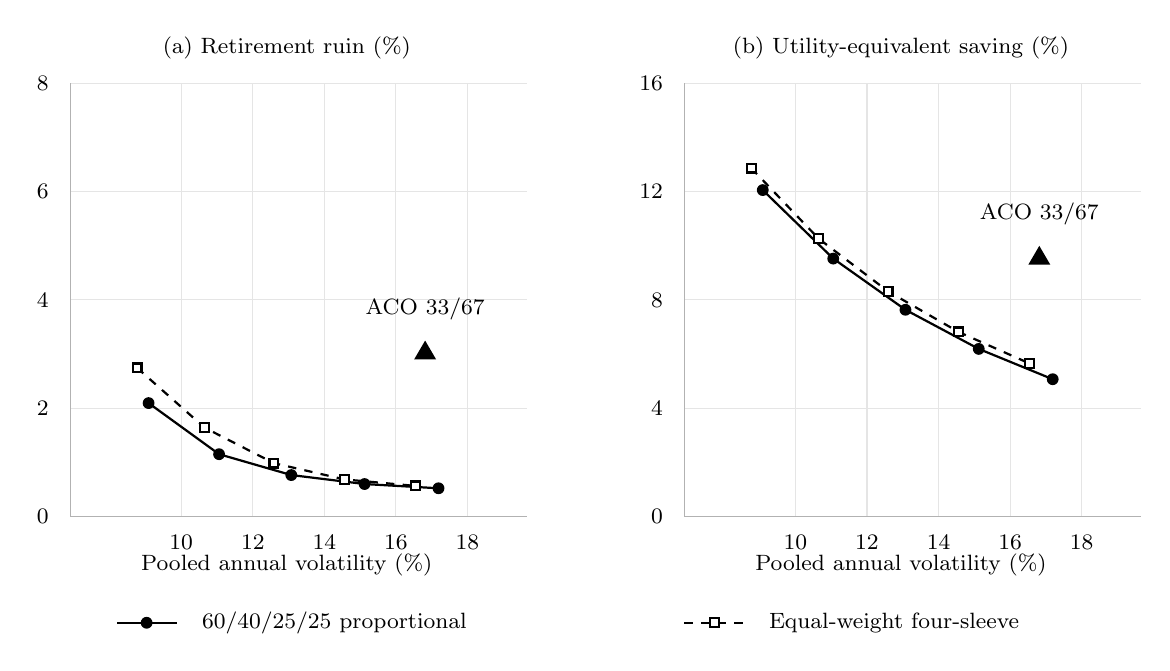
\begin{tikzpicture}[x=1cm, y=1cm]
\begin{scope}[shift={(0.0,0)}]
  \draw[gray!20] (0,0.000) -- (5.80,0.000);
  \node[left, font=\footnotesize] at (-0.15,0.000) {0};
  \draw[gray!20] (0,1.375) -- (5.80,1.375);
  \node[left, font=\footnotesize] at (-0.15,1.375) {2};
  \draw[gray!20] (0,2.750) -- (5.80,2.750);
  \node[left, font=\footnotesize] at (-0.15,2.750) {4};
  \draw[gray!20] (0,4.125) -- (5.80,4.125);
  \node[left, font=\footnotesize] at (-0.15,4.125) {6};
  \draw[gray!20] (0,5.500) -- (5.80,5.500);
  \node[left, font=\footnotesize] at (-0.15,5.500) {8};
  \draw[gray!20] (1.409,0) -- (1.409,5.500);
  \node[below, font=\footnotesize] at (1.409,-0.12) {10};
  \draw[gray!20] (2.318,0) -- (2.318,5.500);
  \node[below, font=\footnotesize] at (2.318,-0.12) {12};
  \draw[gray!20] (3.227,0) -- (3.227,5.500);
  \node[below, font=\footnotesize] at (3.227,-0.12) {14};
  \draw[gray!20] (4.136,0) -- (4.136,5.500);
  \node[below, font=\footnotesize] at (4.136,-0.12) {16};
  \draw[gray!20] (5.045,0) -- (5.045,5.500);
  \node[below, font=\footnotesize] at (5.045,-0.12) {18};
  \draw[gray!60] (0,0) -- (5.80,0);
  \draw[gray!60] (0,0) -- (0,5.500);
  \fill (4.507,2.234) -- ++(-0.14,-0.24) -- ++(0.28,0) -- cycle;
  \node[font=\footnotesize, anchor=south] at (4.507,2.374) {ACO 33/67};
  \draw[thick] plot coordinates {(0.995,1.440) (1.890,0.791) (2.807,0.526) (3.738,0.412) (4.677,0.358)};
  \fill (0.995,1.440) circle (0.075);
  \fill (1.890,0.791) circle (0.075);
  \fill (2.807,0.526) circle (0.075);
  \fill (3.738,0.412) circle (0.075);
  \fill (4.677,0.358) circle (0.075);
  \draw[thick, dashed] plot coordinates {(0.849,1.887) (1.706,1.128) (2.586,0.677) (3.480,0.471) (4.383,0.388)};
  \node[draw, thick, rectangle, inner sep=1.6pt, fill=white] at (0.849,1.887) {};
  \node[draw, thick, rectangle, inner sep=1.6pt, fill=white] at (1.706,1.128) {};
  \node[draw, thick, rectangle, inner sep=1.6pt, fill=white] at (2.586,0.677) {};
  \node[draw, thick, rectangle, inner sep=1.6pt, fill=white] at (3.480,0.471) {};
  \node[draw, thick, rectangle, inner sep=1.6pt, fill=white] at (4.383,0.388) {};
  \node[font=\footnotesize] at (2.75,5.95) {(a) Retirement ruin (\%)};
  \node[font=\footnotesize] at (2.75,-0.62) {Pooled annual volatility (\%)};
\end{scope}
\begin{scope}[shift={(7.8,0)}]
  \draw[gray!20] (0,0.000) -- (5.80,0.000);
  \node[left, font=\footnotesize] at (-0.15,0.000) {0};
  \draw[gray!20] (0,1.375) -- (5.80,1.375);
  \node[left, font=\footnotesize] at (-0.15,1.375) {4};
  \draw[gray!20] (0,2.750) -- (5.80,2.750);
  \node[left, font=\footnotesize] at (-0.15,2.750) {8};
  \draw[gray!20] (0,4.125) -- (5.80,4.125);
  \node[left, font=\footnotesize] at (-0.15,4.125) {12};
  \draw[gray!20] (0,5.500) -- (5.80,5.500);
  \node[left, font=\footnotesize] at (-0.15,5.500) {16};
  \draw[gray!20] (1.409,0) -- (1.409,5.500);
  \node[below, font=\footnotesize] at (1.409,-0.12) {10};
  \draw[gray!20] (2.318,0) -- (2.318,5.500);
  \node[below, font=\footnotesize] at (2.318,-0.12) {12};
  \draw[gray!20] (3.227,0) -- (3.227,5.500);
  \node[below, font=\footnotesize] at (3.227,-0.12) {14};
  \draw[gray!20] (4.136,0) -- (4.136,5.500);
  \node[below, font=\footnotesize] at (4.136,-0.12) {16};
  \draw[gray!20] (5.045,0) -- (5.045,5.500);
  \node[below, font=\footnotesize] at (5.045,-0.12) {18};
  \draw[gray!60] (0,0) -- (5.80,0);
  \draw[gray!60] (0,0) -- (0,5.500);
  \fill (4.507,3.437) -- ++(-0.14,-0.24) -- ++(0.28,0) -- cycle;
  \node[font=\footnotesize, anchor=south] at (4.507,3.577) {ACO 33/67};
  \draw[thick] plot coordinates {(0.995,4.145) (1.890,3.275) (2.807,2.625) (3.738,2.128) (4.677,1.743)};
  \fill (0.995,4.145) circle (0.075);
  \fill (1.890,3.275) circle (0.075);
  \fill (2.807,2.625) circle (0.075);
  \fill (3.738,2.128) circle (0.075);
  \fill (4.677,1.743) circle (0.075);
  \draw[thick, dashed] plot coordinates {(0.849,4.424) (1.706,3.527) (2.586,2.859) (3.480,2.344) (4.383,1.943)};
  \node[draw, thick, rectangle, inner sep=1.6pt, fill=white] at (0.849,4.424) {};
  \node[draw, thick, rectangle, inner sep=1.6pt, fill=white] at (1.706,3.527) {};
  \node[draw, thick, rectangle, inner sep=1.6pt, fill=white] at (2.586,2.859) {};
  \node[draw, thick, rectangle, inner sep=1.6pt, fill=white] at (3.480,2.344) {};
  \node[draw, thick, rectangle, inner sep=1.6pt, fill=white] at (4.383,1.943) {};
  \node[font=\footnotesize] at (2.75,5.95) {(b) Utility-equivalent saving (\%)};
  \node[font=\footnotesize] at (2.75,-0.62) {Pooled annual volatility (\%)};
\end{scope}
  \draw[thick] (0.60,-1.35) -- (1.35,-1.35);
  \fill (0.97,-1.35) circle (0.075);
  \node[font=\footnotesize, anchor=west] at (1.55,-1.35) {60/40/25/25 proportional};
  \draw[thick, dashed] (7.80,-1.35) -- (8.55,-1.35);
  \node[draw, thick, rectangle, inner sep=1.6pt, fill=white] at (8.18,-1.35) {};
  \node[font=\footnotesize, anchor=west] at (8.75,-1.35) {Equal-weight four-sleeve};
\end{tikzpicture}

\caption{The two ladder families against the ACO benchmark on U.S. country-years only}
\label{fig:ladders-usa}
\begin{minipage}{0.9\textwidth}\footnotesize
\textit{Note:} 20,000 paired simulations on the 99 U.S. country-years,
1927--2025, at the baseline spread and hedging costs. The filled triangle marks
the ACO 33/67 benchmark (pooled volatility 16.81\%, ruin 3.15\%, saving 10\%).
Full recipes in Appendix~\ref{app:numeraire-controls}.
\end{minipage}
\end{figure}


Appendix~\ref{app:numeraire-controls} documents why the dollar helps,
repeats the construction under German and Japanese numeraires, and reports the
full U.S. recipes behind Table~\ref{tab:usa-control}.

Taken together, the two controls give the same verdict. Managed futures stays
ahead of all-equity under both controls, and gold under the fixed-dollar
control, while on U.S. history its edge is near zero. The covered 90/60 is the
marginal case, slightly behind all-equity in resident purchasing power on the
common sample and slightly ahead under both controls, so the pooled switching
of numeraires does not drive the central result. The \emph{levels} do depend on
the numeraire, and materially, which is why the resident-numeraire convention
is part of the portfolio rule rather than a neutral conversion.


\subsection{Financing and hedging-cost sensitivity}
\label{sec:spread-sensitivity}

The levered comparisons price borrowing at a 30-basis-point spread $\phi$ over
the resident bill and currency hedging at a further 10 basis points $\kappa$.
These are modern retail costs, the implied financing rate of a levered or
return-stacked ETF, or of an exchange-traded box spread, plus a developed-market
currency overlay, applied to the full historical return distribution rather than
the terms an investor faced in every past decade. To show the levered results do
not rest on the borrowing number, Table~\ref{tab:spread} re-runs the leverage
sweep with $\phi$ from zero to 100 basis points, $\kappa$ held at its baseline,
and reads off the 1.5$\times$ rung.

\begin{table}[H]
\centering
\caption{Leverage sweep under a range of financing spreads}
\label{tab:spread}
\setlength{\tabcolsep}{6pt}
\small
\begin{tabular}{lrrr}
\toprule
& \multicolumn{3}{c}{Retirement ruin at the 1.5$\times$ rung} \\
Financing spread $\phi$ & 90/60 covered & $+$ 33 MF & $+$ 33 gold \\
\midrule
\emph{ACO 33/67 (all-equity)} & \multicolumn{3}{c}{\emph{7.36\%}} \\
\addlinespace
0 bp & 7.04\% & 1.54\% & 2.96\% \\
15 bp & 7.36\% & 1.57\% & 3.08\% \\
30 bp (baseline) & 7.63\% & 1.62\% & 3.21\% \\
60 bp & 8.12\% & 1.72\% & 3.54\% \\
100 bp & 8.79\% & 1.95\% & 3.86\% \\
\bottomrule
\end{tabular}
\begin{minipage}{0.92\textwidth}\footnotesize
\textit{Note:} 10,000 paired simulations at seed 20260827 on the same
1{,}557-country-year full historical panel as Table~\ref{tab:frontier}. Entries
are retirement-ruin levels in percent, lower is better, at the 1.5$\times$
rung, where realized volatility is 15.7\%, 17.2\%, and 18.7\% for the three
columns. The ACO 33/67 all-equity row is the reference. The equity sleeve is
ACO 33/67 throughout, and only $\phi$, the spread on the financed portion,
changes. The sweep runs in the leverage-sweep machinery of
Table~\ref{tab:frontier} rather than the main pipeline, so its 30-bp row
differs slightly from Table~\ref{tab:lifecycle} (7.63\% versus 7.81\% for the
covered 90/60). Every comparison in the table is internal to the sweep.
\end{minipage}
\end{table}

The managed-futures and gold columns stay far below the ACO line across the
whole range, at roughly 1.5\% to 2.0\% and 3.0\% to 3.9\% ruin against
ACO's 7.36\%, so their advantage over all-equity does not come from the
chosen borrowing markup, and it survives a spread more than three times the
baseline. The grid varies only $\phi$, not the historical real bill, so it is a
sensitivity to a fixed cost, not a test of whether either sleeve pays when
financing is expensive. The covered 90/60 is the sensitive case, drifting from
just below the benchmark to about a point above it by 100 basis points. The
fixed financing assumption can erase that marginal result but not the two
alternative-sleeve ones.

That sweep isolates the 1.5$\times$ rung, whereas the paper's central claim
concerns the two fixed families at 200\% gross exposure. Table~\ref{tab:central-cost-sensitivity}
therefore applies prospective cost stresses directly to those two endpoints,
without changing their weights or re-targeting volatility. The first panel
raises $\phi$ from 30 to 100, 200, and 300 basis points while holding
$\kappa=10$ basis points. The second holds $\phi=30$ basis points and raises
$\kappa$ to 50 and 100 basis points. These are deliberately conservative
fixed-cost haircuts applied to every historical year. They are useful stresses
for a contemporary investor, but not forecasts that current financing or
hedging terms will prevail over a future lifetime, nor assertions that those
terms prevailed in every historical state.

\begin{table}[H]
\centering
\caption{Prospective financing and hedging-cost stress at 200\% gross exposure}
\label{tab:central-cost-sensitivity}
\small\setlength{\tabcolsep}{3.5pt}
\begin{tabular}{lrrrrrr}
\toprule
Stress & $\phi$ & $\kappa$ & \multicolumn{2}{c}{Proportional 200\%} & \multicolumn{2}{c}{Equal-weight 200\%} \\
 & & & Saving & Ruin & Saving & Ruin \\
\midrule
Financing 30 bp & 0.30\% & 0.10\% & 5.09\% & 1.99\% & 5.92\% & 2.60\% \\
Financing 100 bp & 1.00\% & 0.10\% & 6.18\% & 2.65\% & 7.18\% & 3.53\% \\
Financing 200 bp & 2.00\% & 0.10\% & 8.19\% & 4.28\% & 9.55\% & 5.70\% \\
Financing 300 bp & 3.00\% & 0.10\% & 10.98\% & 6.84\% & 12.99\% & 9.27\% \\
\addlinespace
Hedging 10 bp & 0.30\% & 0.10\% & 5.09\% & 1.99\% & 5.92\% & 2.60\% \\
Hedging 50 bp & 0.30\% & 0.50\% & 5.60\% & 2.24\% & 6.60\% & 3.04\% \\
Hedging 100 bp & 0.30\% & 1.00\% & 6.31\% & 2.77\% & 7.59\% & 3.85\% \\
\bottomrule
\end{tabular}
\begin{minipage}{0.97\textwidth}\footnotesize
\textit{Note:} 10{,}000 paired lifecycle paths per row, ten-year mean stationary blocks, full 1{,}557-country-year panel. The financing rows hold $\kappa=10$ bp, and the hedging rows hold $\phi=30$ bp. Both costs are fixed prospective haircuts applied to every historical year, not forecasts of the financing or hedging terms that prevailed in those years. Saving is utility-equivalent relative to ACO 33/67 at 10\%.
\end{minipage}
\end{table}


At 100 basis points of financing spread, both families still improve on ACO in
both lifecycle criteria: the proportional recipe requires 6.44\% saving and
has 2.55\% ruin, and the equal-weight recipe 7.77\% and 3.28\%. At 200 basis
points, the proportional family remains ahead on both (8.55\% and 4.21\%),
whereas the equal-weight family retains its lower ruin (5.89\%) but no longer
its lower required saving (10.36\%). At the deliberately extreme \mbox{300-basis-point}
stress, the proportional family still has slightly lower ruin (7.09\%)
but requires more saving (11.51\%), and the equal-weight family is worse than
ACO on both reported criteria. In contrast, increasing the hedge friction tenfold
to 100 basis points leaves both families ahead on both measures. Thus the
central result is robust to expensive hedge overlays and to a 100-basis-point
financing stress, while its full two-criterion claim is appropriately sensitive
to sustained financing spreads of 200--300 basis points.

\section{Conclusion}

The paper reproduces ACO's first result: internationally diversified equity is
far better than domestic equity. It reaches a different conclusion once the
opportunity set contains diversified fixed income, gold, and managed futures.
The all-equity 33/67 allocation is no longer the most efficient fixed portfolio
rule in the reproduced lifecycle setting.

At comparable annual volatility, two pre-specified four-sleeve families
outperform ACO on both reported lifecycle criteria. Their 200\% endpoints have
17.80\% and 17.02\% annual volatility, essentially ACO's 17.43\%, but
retirement ruin of 1.83\% and 2.51\% rather than 7.36\%, and
utility-equivalent saving rates of 5.32\% and 6.40\% rather than 10\%. This is
the paper's central result. Within the extended opportunity set,
diversification improves both capital preservation and lifecycle utility at the
same broad risk budget.

The comparison is not between two equally fitted portfolios. ACO's 33/67 rule
is the grid-search optimum over its realized panel, while the diversified
families are fixed rules specified before evaluation. The
sleeves and family forms are nevertheless modeling choices. Beating a selected
benchmark with transparent rules makes the result more demanding, not less.

Levering a bond sleeve alone is a useful contrast. Government bonds are not the
weak link ACO's ranking might suggest. A covered global bond block lowers ruin,
saving, and volatility together relative to the local one, by 0.71 point of
ruin on the pooled panel and 0.38 point on U.S. data, the same direction at a
different magnitude. But a levered 90/60 with that block is effectively
tied with all-equity. Whether it edges past depends on the joint distribution
of its asset and real-bill returns, which differs between postwar U.S. history
and the pooled cross-section. For a
sleeve to clearly beat all-equity, the return source it adds must be large
enough, per unit of added risk, to survive the financing drag. Bonds do add
one, the term premium, but a thin one, which is why the levered covered 90/60
ends in a tie. Managed futures add a much larger one, by about four to
five percentage points of ruin under the resident-numeraire convention, and
gold a smaller one, at every rung of the ladder and with the borrowing
spread anywhere from zero to 100 basis points.

The pooled levels are conditional on the resident-numeraire convention. On the
common 1{,}534-state sample, ACO ruin is 7.05\% in resident purchasing power and
3.04\% in fixed dollars, and the alternative-sleeve gaps contract with it. This
does not make dollars the correct construction, since the domestic sleeve stays
that of the sampled source country. No single ruin or saving level in
this paper should be read as convention-free. What is robust is the ordering
that carries the central result: the two diversified families ahead of
all-equity, on both criteria, at matched volatility, and the managed-futures
and gold sleeves below all-equity under both numeraire conventions.

Three conditions bound extrapolation beyond the design. The gold gain is the
least robust. It is a post-1968 phenomenon, since the administered pre-1968
price makes it \emph{raise} ruin, and it is near zero on U.S. data, which lacks
the non-U.S. inflation crises where gold pays. The diversified-family ranking
survives restricting the sample to the post-1950 and post-1970 windows and to
the single-country control. The managed-futures gain is nevertheless more
data-dependent before 1970, when its market coverage is thinner, and the series
is a reconstruction, not an investable index. And every levered
comparison depends on the realized bill series and the assumed spread. The 50\%
short position gains when the ex-post real bill is low and loses when it is
high, and annual data do not identify how that interacts with inflation and the
risky sleeves. A final caveat is economic rather than mechanical. The levered
comparisons apply today's borrowing terms to historical asset premia that were
earned under the leverage aversion \citet{FrazziniPedersen2014} document. As
cheap embedded leverage spreads, that aversion should relax, the demand for
low-volatility sleeves should rise, and part of their historical premium should
compress. The diversified advantage documented here is therefore best read as an
upper bound on what an investor financing at current terms can expect going
forward. The firmest results use none of this. The currency decomposition
carries no leverage cost and no reconstructed series, and the covered 90/60
versus its local counterpart holds financing fixed, though they are still stated
within a chosen numeraire.

The recurring lesson is economic as well as methodological. Once the opportunity
set includes distinct return sources and the risk budget is restored
transparently, the reproduced data favor diversification over ACO's 100\%
equity allocation. Which allocation wins depends on the full set of assets, the
risk budget the comparison is made at, and the units it is made in.

\newpage
\printbibliography

\appendix
\newpage
\section{Asset-Class Return Histories}
\label{app:returns}

Figure~\ref{fig:cumwealth} plots the real growth of one dollar in each asset
class, for a U.S.\ resident, over the full 1927--2025 window. A single residence
is used so that every series shares one numeraire, and other residents differ
only through their own inflation and exchange rates. The vertical axis is
logarithmic, so a straight segment is a constant compound rate and the slope is
that rate.

\begin{figure}[H]
\centering
% Généré par build_appendix_data.py — ne pas éditer à la main.
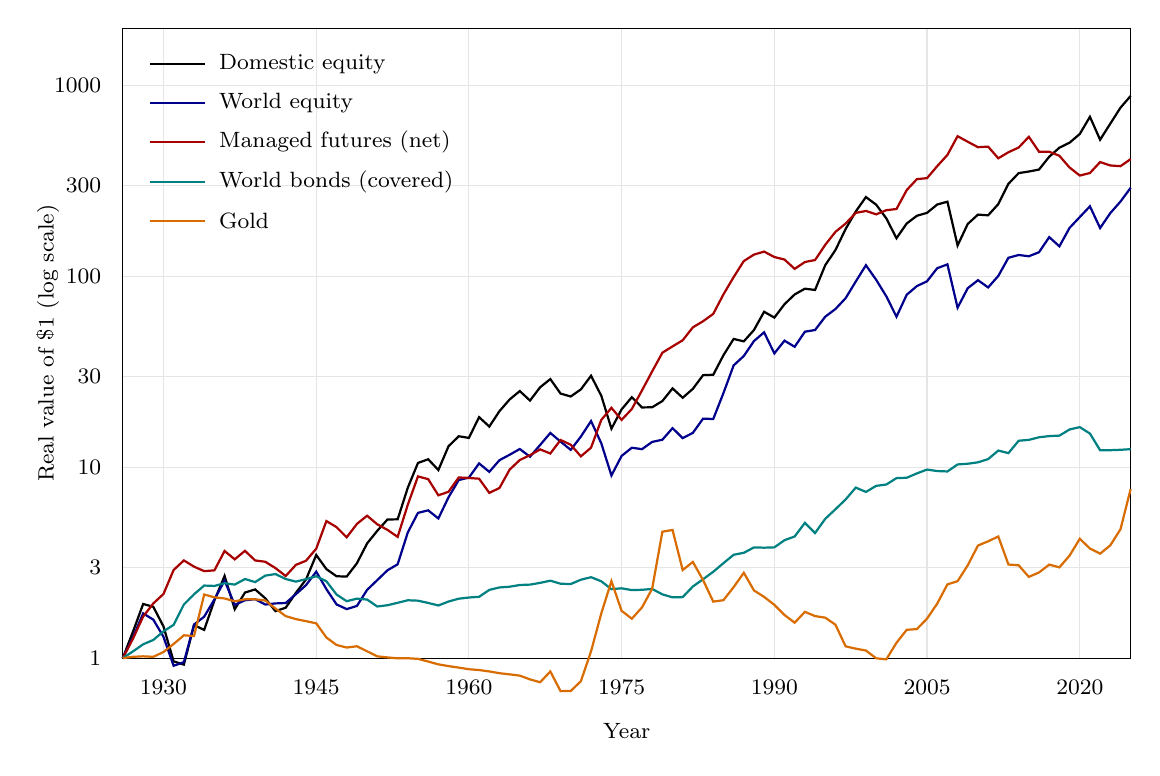
\begin{tikzpicture}[x=1cm, y=1cm]
  \draw[gray!20] (0,0.000) -- (12.80,0.000);
  \node[left, font=\footnotesize] at (-0.15,0.000) {1};
  \draw[gray!20] (0,1.156) -- (12.80,1.156);
  \node[left, font=\footnotesize] at (-0.15,1.156) {3};
  \draw[gray!20] (0,2.423) -- (12.80,2.423);
  \node[left, font=\footnotesize] at (-0.15,2.423) {10};
  \draw[gray!20] (0,3.580) -- (12.80,3.580);
  \node[left, font=\footnotesize] at (-0.15,3.580) {30};
  \draw[gray!20] (0,4.847) -- (12.80,4.847);
  \node[left, font=\footnotesize] at (-0.15,4.847) {100};
  \draw[gray!20] (0,6.003) -- (12.80,6.003);
  \node[left, font=\footnotesize] at (-0.15,6.003) {300};
  \draw[gray!20] (0,7.270) -- (12.80,7.270);
  \node[left, font=\footnotesize] at (-0.15,7.270) {1000};
  \draw[gray!20] (0.517,0) -- (0.517,8.00);
  \node[below, font=\footnotesize] at (0.517,-0.15) {1930};
  \draw[gray!20] (2.457,0) -- (2.457,8.00);
  \node[below, font=\footnotesize] at (2.457,-0.15) {1945};
  \draw[gray!20] (4.396,0) -- (4.396,8.00);
  \node[below, font=\footnotesize] at (4.396,-0.15) {1960};
  \draw[gray!20] (6.335,0) -- (6.335,8.00);
  \node[below, font=\footnotesize] at (6.335,-0.15) {1975};
  \draw[gray!20] (8.275,0) -- (8.275,8.00);
  \node[below, font=\footnotesize] at (8.275,-0.15) {1990};
  \draw[gray!20] (10.214,0) -- (10.214,8.00);
  \node[below, font=\footnotesize] at (10.214,-0.15) {2005};
  \draw[gray!20] (12.154,0) -- (12.154,8.00);
  \node[below, font=\footnotesize] at (12.154,-0.15) {2020};
  \draw (0,0) rectangle (12.80,8.00);
  \node[below, font=\footnotesize] at (6.40,-0.7) {Year};
  \node[rotate=90, font=\footnotesize] at (-0.95,4.00) {Real value of \$1 (log scale)};
  \draw[thick, black] plot coordinates {(0.000,0.000) (0.129,0.335) (0.259,0.688) (0.388,0.652) (0.517,0.403) (0.646,-0.041) (0.776,-0.082) (0.905,0.419) (1.034,0.359) (1.164,0.733) (1.293,1.044) (1.422,0.621) (1.552,0.833) (1.681,0.873) (1.810,0.760) (1.939,0.597) (2.069,0.640) (2.198,0.828) (2.327,0.999) (2.457,1.310) (2.586,1.131) (2.715,1.040) (2.844,1.036) (2.974,1.206) (3.103,1.457) (3.232,1.617) (3.362,1.761) (3.491,1.763) (3.620,2.165) (3.749,2.479) (3.879,2.526) (4.008,2.389) (4.137,2.691) (4.267,2.818) (4.396,2.797) (4.525,3.061) (4.655,2.941) (4.784,3.137) (4.913,3.285) (5.042,3.392) (5.172,3.271) (5.301,3.441) (5.430,3.544) (5.560,3.360) (5.689,3.323) (5.818,3.413) (5.947,3.586) (6.077,3.333) (6.206,2.914) (6.335,3.159) (6.465,3.314) (6.594,3.184) (6.723,3.186) (6.853,3.265) (6.982,3.426) (7.111,3.307) (7.240,3.420) (7.370,3.594) (7.499,3.599) (7.628,3.846) (7.758,4.054) (7.887,4.023) (8.016,4.167) (8.145,4.399) (8.275,4.325) (8.404,4.495) (8.533,4.619) (8.663,4.692) (8.792,4.676) (8.921,4.990) (9.051,5.183) (9.180,5.450) (9.309,5.673) (9.438,5.856) (9.568,5.759) (9.697,5.585) (9.826,5.333) (9.956,5.520) (10.085,5.618) (10.214,5.655) (10.343,5.761) (10.473,5.797) (10.602,5.241) (10.731,5.514) (10.861,5.633) (10.990,5.624) (11.119,5.766) (11.248,6.024) (11.378,6.160) (11.507,6.180) (11.636,6.205) (11.766,6.368) (11.895,6.483) (12.024,6.546) (12.154,6.657) (12.283,6.875) (12.412,6.584) (12.541,6.787) (12.671,6.991) (12.800,7.140)};
  \draw[thick, blue!55!black] plot coordinates {(0.000,0.000) (0.129,0.266) (0.259,0.568) (0.388,0.489) (0.517,0.271) (0.646,-0.097) (0.776,-0.051) (0.905,0.426) (1.034,0.527) (1.164,0.746) (1.293,0.985) (1.422,0.676) (1.552,0.735) (1.681,0.749) (1.810,0.681) (1.939,0.695) (2.069,0.700) (2.198,0.812) (2.327,0.927) (2.457,1.098) (2.586,0.877) (2.715,0.682) (2.844,0.623) (2.974,0.663) (3.103,0.867) (3.232,0.991) (3.362,1.116) (3.491,1.192) (3.620,1.597) (3.749,1.845) (3.879,1.877) (4.008,1.774) (4.137,2.043) (4.267,2.262) (4.396,2.293) (4.525,2.473) (4.655,2.366) (4.784,2.514) (4.913,2.583) (5.042,2.656) (5.172,2.558) (5.301,2.708) (5.430,2.860) (5.560,2.750) (5.689,2.645) (5.818,2.814) (5.947,3.011) (6.077,2.729) (6.206,2.320) (6.335,2.568) (6.465,2.672) (6.594,2.654) (6.723,2.746) (6.853,2.774) (6.982,2.921) (7.111,2.794) (7.240,2.861) (7.370,3.042) (7.499,3.037) (7.628,3.365) (7.758,3.718) (7.887,3.837) (8.016,4.027) (8.145,4.138) (8.275,3.870) (8.404,4.032) (8.533,3.954) (8.663,4.146) (8.792,4.167) (8.921,4.336) (9.051,4.434) (9.180,4.571) (9.309,4.783) (9.438,4.990) (9.568,4.805) (9.697,4.595) (9.826,4.336) (9.956,4.615) (10.085,4.725) (10.214,4.786) (10.343,4.952) (10.473,5.001) (10.602,4.451) (10.731,4.698) (10.861,4.800) (10.990,4.708) (11.119,4.854) (11.248,5.085) (11.378,5.120) (11.507,5.104) (11.636,5.155) (11.766,5.347) (11.895,5.230) (12.024,5.464) (12.154,5.602) (12.283,5.738) (12.412,5.462) (12.541,5.651) (12.671,5.799) (12.800,5.973)};
  \draw[thick, red!65!black] plot coordinates {(0.000,0.000) (0.129,0.246) (0.259,0.528) (0.388,0.695) (0.517,0.815) (0.646,1.120) (0.776,1.241) (0.905,1.162) (1.034,1.105) (1.164,1.115) (1.293,1.361) (1.422,1.255) (1.552,1.363) (1.681,1.241) (1.810,1.224) (1.939,1.144) (2.069,1.043) (2.198,1.184) (2.327,1.237) (2.457,1.390) (2.586,1.741) (2.715,1.664) (2.844,1.535) (2.974,1.705) (3.103,1.809) (3.232,1.700) (3.362,1.629) (3.491,1.540) (3.620,1.949) (3.749,2.308) (3.879,2.273) (4.008,2.068) (4.137,2.113) (4.267,2.295) (4.396,2.288) (4.525,2.279) (4.655,2.099) (4.784,2.161) (4.913,2.394) (5.042,2.516) (5.172,2.578) (5.301,2.651) (5.430,2.599) (5.560,2.771) (5.689,2.710) (5.818,2.563) (5.947,2.673) (6.077,3.025) (6.206,3.179) (6.335,3.026) (6.465,3.164) (6.594,3.400) (6.723,3.641) (6.853,3.879) (6.982,3.959) (7.111,4.037) (7.240,4.201) (7.370,4.279) (7.499,4.372) (7.628,4.619) (7.758,4.839) (7.887,5.043) (8.016,5.125) (8.145,5.163) (8.275,5.094) (8.404,5.062) (8.533,4.944) (8.663,5.031) (8.792,5.056) (8.921,5.249) (9.051,5.414) (9.180,5.519) (9.309,5.655) (9.438,5.679) (9.568,5.636) (9.697,5.689) (9.826,5.704) (9.956,5.944) (10.085,6.083) (10.214,6.096) (10.343,6.248) (10.473,6.391) (10.602,6.629) (10.731,6.558) (10.861,6.489) (10.990,6.496) (11.119,6.348) (11.248,6.425) (11.378,6.485) (11.507,6.621) (11.636,6.432) (11.766,6.431) (11.895,6.380) (12.024,6.231) (12.154,6.129) (12.283,6.161) (12.412,6.300) (12.541,6.257) (12.671,6.248) (12.800,6.338)};
  \draw[thick, teal] plot coordinates {(0.000,0.000) (0.129,0.085) (0.259,0.176) (0.388,0.231) (0.517,0.340) (0.646,0.423) (0.776,0.681) (0.905,0.811) (1.034,0.922) (1.164,0.917) (1.293,0.952) (1.422,0.934) (1.552,1.005) (1.681,0.966) (1.810,1.048) (1.939,1.068) (2.069,1.005) (2.198,0.972) (2.327,1.004) (2.457,1.040) (2.586,0.976) (2.715,0.808) (2.844,0.723) (2.974,0.756) (3.103,0.744) (3.232,0.656) (3.362,0.672) (3.491,0.703) (3.620,0.735) (3.749,0.730) (3.879,0.701) (4.008,0.669) (4.137,0.719) (4.267,0.755) (4.396,0.770) (4.525,0.779) (4.655,0.867) (4.784,0.898) (4.913,0.907) (5.042,0.929) (5.172,0.934) (5.301,0.956) (5.430,0.984) (5.560,0.945) (5.689,0.941) (5.818,0.996) (5.947,1.028) (6.077,0.976) (6.206,0.876) (6.335,0.887) (6.465,0.864) (6.594,0.868) (6.723,0.879) (6.853,0.810) (6.982,0.772) (7.111,0.775) (7.240,0.910) (7.370,1.002) (7.499,1.097) (7.628,1.206) (7.758,1.313) (7.887,1.338) (8.016,1.406) (8.145,1.403) (8.275,1.407) (8.404,1.498) (8.533,1.545) (8.663,1.718) (8.792,1.589) (8.921,1.769) (9.051,1.891) (9.180,2.015) (9.309,2.166) (9.438,2.111) (9.568,2.188) (9.697,2.205) (9.826,2.286) (9.956,2.291) (10.085,2.346) (10.214,2.395) (10.343,2.376) (10.473,2.371) (10.602,2.460) (10.731,2.469) (10.861,2.487) (10.990,2.528) (11.119,2.636) (11.248,2.604) (11.378,2.761) (11.507,2.772) (11.636,2.805) (11.766,2.820) (11.895,2.826) (12.024,2.904) (12.154,2.934) (12.283,2.852) (12.412,2.641) (12.541,2.641) (12.671,2.646) (12.800,2.654)};
  \draw[thick, orange!85!black] plot coordinates {(0.000,0.000) (0.129,0.017) (0.259,0.023) (0.388,0.017) (0.517,0.078) (0.646,0.180) (0.776,0.290) (0.905,0.281) (1.034,0.808) (1.164,0.773) (1.293,0.758) (1.422,0.722) (1.552,0.747) (1.681,0.747) (1.810,0.732) (1.939,0.630) (2.069,0.534) (2.198,0.496) (2.327,0.470) (2.457,0.442) (2.586,0.262) (2.715,0.167) (2.844,0.135) (2.974,0.151) (3.103,0.087) (3.232,0.023) (3.362,0.009) (3.491,-0.002) (3.620,-0.001) (3.749,-0.009) (3.879,-0.043) (4.008,-0.079) (4.137,-0.101) (4.267,-0.120) (4.396,-0.141) (4.525,-0.151) (4.655,-0.169) (4.784,-0.191) (4.913,-0.206) (5.042,-0.222) (5.172,-0.270) (5.301,-0.306) (5.430,-0.169) (5.560,-0.419) (5.689,-0.417) (5.818,-0.293) (5.947,0.086) (6.077,0.568) (6.206,0.978) (6.335,0.601) (6.465,0.501) (6.594,0.644) (6.723,0.881) (6.853,1.606) (6.982,1.628) (7.111,1.119) (7.240,1.222) (7.370,0.991) (7.499,0.718) (7.628,0.736) (7.758,0.902) (7.887,1.084) (8.016,0.860) (8.145,0.778) (8.275,0.677) (8.404,0.548) (8.533,0.450) (8.663,0.588) (8.792,0.534) (8.921,0.514) (9.051,0.425) (9.180,0.150) (9.309,0.120) (9.438,0.097) (9.568,-0.002) (9.697,-0.015) (9.826,0.195) (9.956,0.360) (10.085,0.369) (10.214,0.502) (10.343,0.692) (10.473,0.937) (10.602,0.977) (10.731,1.179) (10.861,1.430) (10.990,1.484) (11.119,1.545) (11.248,1.189) (11.378,1.179) (11.507,1.032) (11.636,1.088) (11.766,1.188) (11.895,1.153) (12.024,1.302) (12.154,1.516) (12.283,1.392) (12.412,1.327) (12.541,1.432) (12.671,1.637) (12.800,2.148)};
  \draw[thick, black] (0.35,7.550) -- (1.05,7.550);
  \node[right, font=\footnotesize] at (1.1,7.550) {Domestic equity};
  \draw[thick, blue!55!black] (0.35,7.050) -- (1.05,7.050);
  \node[right, font=\footnotesize] at (1.1,7.050) {World equity};
  \draw[thick, red!65!black] (0.35,6.550) -- (1.05,6.550);
  \node[right, font=\footnotesize] at (1.1,6.550) {Managed futures (net)};
  \draw[thick, teal] (0.35,6.050) -- (1.05,6.050);
  \node[right, font=\footnotesize] at (1.1,6.050) {World bonds (covered)};
  \draw[thick, orange!85!black] (0.35,5.550) -- (1.05,5.550);
  \node[right, font=\footnotesize] at (1.1,5.550) {Gold};
\end{tikzpicture}

\caption{Cumulative real return by asset class, U.S.\ resident, 1927--2025.
Managed futures are the reconstructed time-series-momentum proxy net of the
0.85\% fee and 0.57\% turnover cost. World bonds are the covered equal-weight
basket of all panel sovereigns. Gold is the spliced MeasuringWorth--LBMA price less custody.
Equity and gold are unhedged, while bonds and managed futures are currency-hedged
under covered interest parity. The managed-futures proxy compounds at close to
the equity rate over the century, but its decade-by-decade path is far more
volatile before 1960, when the underlying market set is thin.}
\label{fig:cumwealth}
\end{figure}

The managed-futures line ends near the world-equity line, so the proxy is not a
weak long-run performer. Its pre-1960 segment is visibly steeper and rougher
than its post-1970 segment, because the proxy's internal 36-month volatility
scaling (Section~\ref{sec:data}) has few markets to work with early in the
sample, which inflates realized volatility without raising the mean. This is the construction
feature behind the pre-1970 weakness of the levered multi-asset portfolios in
the main text, alongside the low and volatile real cash and bond returns of the
same decades.

\section{Properties of the reconstructed managed-futures proxy}
\label{app:mf-proxy}

The managed-futures sleeve is the only asset class we build rather than take
from a published series, so this appendix does two things. It benchmarks the
proxy against commercial trend-following indexes
(Appendix~\ref{app:mf-external}), and it sets out its annual return properties
against the other asset classes, including its behavior when equities fall
(Appendix~\ref{app:mf-annual}).

The construction is described in Section~\ref{sec:data}. In brief, it is the
time-series-momentum rule of \citet{MoskowitzOoiPedersen2012}, in the
multi-speed, century-length form of \citet{HurstOoiPedersen2017}: each market
carries a position equal to the sign of a blend of its one-, six-, and
twelve-month past returns, scaled to a target volatility, and the sleeve is the
inverse-volatility average across four sectors. \citet{BaltasKosowski2020}
motivate the choice of signal horizon and the turnover-based cost, and
\citet{LempiereEtAl2014} document a trend premium across asset classes back to
1800, which is what justifies running the rule over 1927--2025. Section~%
\ref{sec:data} reports the sector Sharpe ratios of the reconstruction against
the Capital Fund Management estimates of \citet{LempiereEtAl2014} (0.77 versus
0.80 combined).

\subsection{Monthly inputs and the annual simulation series}
\label{app:mf-monthly-data}

There are two deliberately separate data layers. The JST/Macrohistory file
used by the lifecycle experiment is annual. It supplies the resident-specific
equity, bond, bill, inflation, and exchange-rate returns that are resampled in
the bootstrap, and it is not used to manufacture monthly observations. The MF
sleeve starts instead from a frozen monthly snapshot covering January 1921 to
December 2025. The snapshot contains nominal monthly returns only: no
inflation adjustment, fees, interpolation, or return calculated across a
change of source. It is a separate input to the trading rule, not an
additional frequency dimension in the lifecycle simulation.

These monthly data reconstruct a trend signal, not a wealth path, and we do
not use them to re-run the lifecycle experiment. Three gaps explain why.
First, equity segments are price returns with no dividends. The roughly three
to five annual points this omits are close to irrelevant for the sign of a
momentum signal, but they would be decisive in a retirement-ruin calculation,
which compounds the drift over three decades. Second, bond segments are par
ten-year excess returns implied from yield levels. That is an adequate proxy
for the direction of a bond market, but not the total return that funds a
pension. Third, exchange rates begin only in 1971, and the file carries a
U.S. deflator alone, so it cannot express a return in a non-U.S. resident's
purchasing power before then. The annual Macrohistory panel has none of these
limitations---dividend-inclusive equity total returns, observed bond total
returns, and resident-specific inflation and exchange rates over the full 1927
window---which is why the bootstrap continues to draw from it.

\begin{table}[H]
\centering
\caption{Monthly data used to construct the managed-futures proxy}
\label{tab:mf-monthly-sources}
\small
\begin{tabular}{>{\raggedright\arraybackslash}p{0.16\textwidth}>{\raggedright\arraybackslash}p{0.53\textwidth}>{\raggedright\arraybackslash}p{0.20\textwidth}}
\toprule
Input & Monthly source and transformation & What enters the MF rule \\
\midrule
Equities & National price indexes from OECD Main Economic Indicators via FRED, and before their availability, the U.S., U.K., German, and French NBER Macrohistory monthly price series. & 18 local-currency price returns. Dividends are absent. \\
Rates & Monthly sovereign yields from OECD via FRED, augmented before their start by NBER U.S. yields, U.K. Consol/Bank of England yields, and the French 3\% rente. Each yield pair is priced as a par ten-year bond, then the lagged three-month cash return is subtracted. & 18 synthetic local-currency bond excess returns, not changes in yields and not observed futures returns. \\
Commodities & NBER/BLS monthly wholesale prices for the early history and the World Bank Pink Sheet from 1960. Gold uses the official U.S. price before 1960 and the Pink Sheet thereafter, and silver starts in 1960. & 19 commodity spot-price returns plus gold and silver. Carry, basis, and futures roll are unavailable and therefore set to zero. \\
Currencies & Board of Governors H.10 daily dollar quotations via FRED, reduced to the last available observation in each month, with a lagged three-month interest differential forming a synthetic forward excess return. & AUD, CAD, CHF, GBP, JPY from 1971 and EUR from 1999. Earlier European currencies are not backfilled. \\
Collateral and deflator & Monthly three-month cash rates from OECD via FRED, with a lagged prior-year JST/GMD fallback only where monthly rates do not exist, plus monthly U.S. CPI for deflation. & U.S. cash collateral is added once to the USD MF NAV, and CPI converts the final monthly USD return to real terms. \\
\bottomrule
\end{tabular}
\begin{minipage}{0.94\textwidth}\footnotesize
\textit{Note:} The machine-readable source-segment file records the provider,
series identifier, dates, transformation, and source seam for every market.
The source list is intentionally more granular than the annual Macrohistory
panel: the latter cannot identify a month-end trading signal. The monthly
snapshot is frozen for this replication, and source seams receive no return in the
first month of a new segment, so a signal cannot cross them silently.
\end{minipage}
\end{table}

At each month $t$, each market's one-, six-, and twelve-month momentum signs
are computed only from the monthly snapshot. Timing requires one point of
care. Some price series are reported as monthly averages rather than
month-end observations. For these, the signal stops at $t-2$: month $t-1$ is
deliberately skipped, because using it would let the signal overlap two
monthly averages. End-of-month currency quotes from the H.10 release need no
such skip. The 36-month volatility estimate and the inverse-volatility sector
weights are lagged the same way, so every input to a position is known at the
time the position is taken.

Local equity and bond P\&L is converted to U.S.\ dollars only when the
corresponding H.10 spot rate exists; otherwise that market is absent for the
month. Thus neither a missing exchange rate nor a source change is implicitly
treated as a zero return.

The monthly engine first produces a nominal U.S.-dollar MF return each month
and records the U.S.\ cash-collateral return separately. The path from monthly
to annual is then mechanical. Each monthly return is deflated by the
contemporaneous U.S. CPI, the twelve real monthly returns within a calendar
year are compounded, and a year enters the annual simulation file only if all
twelve monthly returns and all twelve CPI observations exist---no partial year
is annualized. One last link closes the loop. The monthly sleeve embeds U.S.\
collateral; the household panel removes it under covered interest parity and
replaces it with the resident's own bill. The monthly data therefore determine
the MF signal and its annual return, whereas the country-year bootstrap
continues to operate exclusively on annual resident-real returns.

\subsection{Comparison with commercial trend-following indexes}
\label{app:mf-external}

The proxy is calibrated only to public price data and a fixed rule, and it is
not fitted to any managed-futures index. As an external check,
Figure~\ref{fig:mf-vs-benchmarks} plots the growth of one dollar in the net
proxy against the SG CTA, SG Trend, and Barclay BTOP50 indexes
\citep{SGIndices,BTOP50} and the KMLMSIM Testfolio simulation \citep{Testfol}
over 2000--2025, the common window imposed by the SG series. KMLMSIM follows
the KFA MLM Index less 0.90\% per year before 2020 and the live KMLM ETF
thereafter. The proxy tracks the same broad path, with end multiples of
3.8$\times$ for the proxy against 2.8$\times$ to 3.9$\times$ for the three
commercial indexes, and the same major inflections in 2008, 2014--15, and
2022. The one
sustained divergence is 2019--2020, when the proxy loses about 18\% cumulatively
while the indexes gain about 13\%. Both years turned on fast reversals, the 2019
Fed pivot and the March-2020 crash and V-shaped recovery, which a monthly
reconstruction with a one-month signal lag and end-of-month currency conversion
takes on the wrong foot, exactly the annual-data limitation noted in
Section~\ref{sec:data}. Over the full window the proxy still ends within the
index range.

\begin{figure}[H]
\centering
% Généré par build_mf_benchmark_data.py — ne pas éditer à la main.
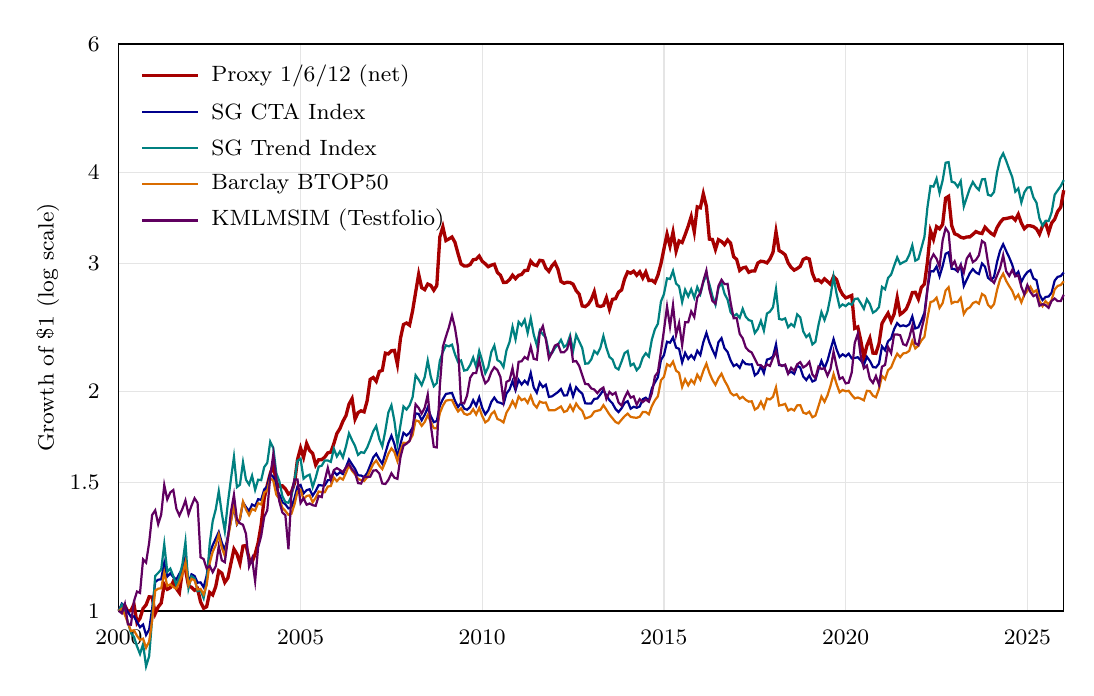
\begin{tikzpicture}[x=1cm, y=1cm]
  \draw[gray!20] (0,0.000) -- (12.00,0.000);
  \node[left, font=\footnotesize] at (-0.12,0.000) {1};
  \draw[gray!20] (0,1.629) -- (12.00,1.629);
  \node[left, font=\footnotesize] at (-0.12,1.629) {1.5};
  \draw[gray!20] (0,2.785) -- (12.00,2.785);
  \node[left, font=\footnotesize] at (-0.12,2.785) {2};
  \draw[gray!20] (0,4.415) -- (12.00,4.415);
  \node[left, font=\footnotesize] at (-0.12,4.415) {3};
  \draw[gray!20] (0,5.571) -- (12.00,5.571);
  \node[left, font=\footnotesize] at (-0.12,5.571) {4};
  \draw[gray!20] (0,7.200) -- (12.00,7.200);
  \node[left, font=\footnotesize] at (-0.12,7.200) {6};
  \draw[gray!20] (0.000,0) -- (0.000,7.20);
  \node[below, font=\footnotesize] at (0.000,-0.12) {2000};
  \draw[gray!20] (2.308,0) -- (2.308,7.20);
  \node[below, font=\footnotesize] at (2.308,-0.12) {2005};
  \draw[gray!20] (4.615,0) -- (4.615,7.20);
  \node[below, font=\footnotesize] at (4.615,-0.12) {2010};
  \draw[gray!20] (6.923,0) -- (6.923,7.20);
  \node[below, font=\footnotesize] at (6.923,-0.12) {2015};
  \draw[gray!20] (9.231,0) -- (9.231,7.20);
  \node[below, font=\footnotesize] at (9.231,-0.12) {2020};
  \draw[gray!20] (11.538,0) -- (11.538,7.20);
  \node[below, font=\footnotesize] at (11.538,-0.12) {2025};
  \draw (0,0) rectangle (12.00,7.20);
  \node[rotate=90, font=\footnotesize] at (-0.9,3.60) {Growth of \$1 (log scale)};
  \draw[very thick, red!65!black] plot coordinates {(0.000,0.000) (0.038,0.063) (0.077,0.069) (0.115,-0.008) (0.154,0.007) (0.192,0.085) (0.231,-0.150) (0.269,-0.094) (0.308,0.032) (0.346,0.077) (0.385,0.180) (0.423,0.176) (0.462,-0.033) (0.500,0.052) (0.538,0.100) (0.577,0.336) (0.615,0.275) (0.654,0.296) (0.692,0.376) (0.731,0.284) (0.769,0.230) (0.808,0.514) (0.846,0.527) (0.885,0.320) (0.923,0.300) (0.962,0.263) (1.000,0.282) (1.038,0.115) (1.077,0.034) (1.115,0.054) (1.154,0.235) (1.192,0.204) (1.231,0.311) (1.269,0.509) (1.308,0.480) (1.346,0.363) (1.385,0.420) (1.423,0.602) (1.462,0.786) (1.500,0.723) (1.538,0.605) (1.577,0.824) (1.615,0.832) (1.654,0.667) (1.692,0.622) (1.731,0.722) (1.769,0.865) (1.808,1.097) (1.846,1.430) (1.885,1.596) (1.923,1.744) (1.962,1.857) (2.000,1.630) (2.038,1.583) (2.077,1.590) (2.115,1.551) (2.154,1.484) (2.192,1.510) (2.231,1.621) (2.269,1.922) (2.308,2.069) (2.346,1.951) (2.385,2.126) (2.423,2.039) (2.462,2.000) (2.500,1.855) (2.538,1.921) (2.577,1.922) (2.615,1.953) (2.654,2.008) (2.692,2.017) (2.731,2.125) (2.769,2.253) (2.808,2.316) (2.846,2.409) (2.885,2.481) (2.923,2.626) (2.962,2.696) (3.000,2.436) (3.038,2.519) (3.077,2.542) (3.115,2.528) (3.154,2.671) (3.192,2.941) (3.231,2.965) (3.269,2.916) (3.308,3.041) (3.346,3.056) (3.385,3.274) (3.423,3.264) (3.462,3.305) (3.500,3.309) (3.538,3.132) (3.577,3.463) (3.615,3.638) (3.654,3.657) (3.692,3.629) (3.731,3.813) (3.769,4.045) (3.808,4.276) (3.846,4.106) (3.885,4.081) (3.923,4.152) (3.962,4.134) (4.000,4.073) (4.038,4.133) (4.077,4.751) (4.115,4.878) (4.154,4.704) (4.192,4.725) (4.231,4.749) (4.269,4.681) (4.308,4.537) (4.346,4.408) (4.385,4.381) (4.423,4.381) (4.462,4.400) (4.500,4.460) (4.538,4.467) (4.577,4.507) (4.615,4.441) (4.654,4.409) (4.692,4.372) (4.731,4.392) (4.769,4.403) (4.808,4.298) (4.846,4.264) (4.885,4.172) (4.923,4.174) (4.962,4.208) (5.000,4.264) (5.038,4.220) (5.077,4.263) (5.115,4.273) (5.154,4.324) (5.192,4.326) (5.231,4.442) (5.269,4.399) (5.308,4.386) (5.346,4.453) (5.385,4.446) (5.423,4.355) (5.462,4.313) (5.500,4.382) (5.538,4.425) (5.577,4.338) (5.615,4.185) (5.654,4.162) (5.692,4.174) (5.731,4.171) (5.769,4.150) (5.808,4.068) (5.846,4.024) (5.885,3.874) (5.923,3.865) (5.962,3.895) (6.000,3.955) (6.038,4.053) (6.077,3.878) (6.115,3.867) (6.154,3.879) (6.192,3.978) (6.231,3.833) (6.269,3.957) (6.308,3.966) (6.346,4.048) (6.385,4.077) (6.423,4.217) (6.462,4.306) (6.500,4.289) (6.538,4.315) (6.577,4.264) (6.615,4.307) (6.654,4.230) (6.692,4.305) (6.731,4.196) (6.769,4.201) (6.808,4.171) (6.846,4.263) (6.885,4.410) (6.923,4.599) (6.962,4.785) (7.000,4.634) (7.038,4.811) (7.077,4.570) (7.115,4.699) (7.154,4.679) (7.192,4.778) (7.231,4.887) (7.269,5.009) (7.308,4.814) (7.346,5.132) (7.385,5.120) (7.423,5.298) (7.462,5.138) (7.500,4.722) (7.538,4.718) (7.577,4.591) (7.615,4.715) (7.654,4.692) (7.692,4.652) (7.731,4.712) (7.769,4.672) (7.808,4.499) (7.846,4.465) (7.885,4.325) (7.923,4.356) (7.962,4.366) (8.000,4.301) (8.038,4.318) (8.077,4.319) (8.115,4.418) (8.154,4.442) (8.192,4.436) (8.231,4.420) (8.269,4.469) (8.308,4.555) (8.346,4.817) (8.385,4.576) (8.423,4.555) (8.462,4.523) (8.500,4.421) (8.538,4.364) (8.577,4.328) (8.615,4.348) (8.654,4.377) (8.692,4.465) (8.731,4.484) (8.769,4.469) (8.808,4.288) (8.846,4.196) (8.885,4.204) (8.923,4.173) (8.962,4.218) (9.000,4.185) (9.038,4.150) (9.077,4.248) (9.115,4.210) (9.154,4.088) (9.192,4.018) (9.231,3.976) (9.269,3.990) (9.308,4.007) (9.346,3.589) (9.385,3.607) (9.423,3.433) (9.462,3.213) (9.500,3.368) (9.538,3.463) (9.577,3.275) (9.615,3.272) (9.654,3.396) (9.692,3.651) (9.731,3.720) (9.769,3.781) (9.808,3.680) (9.846,3.771) (9.885,3.978) (9.923,3.767) (9.962,3.795) (10.000,3.835) (10.038,3.924) (10.077,4.043) (10.115,4.047) (10.154,3.962) (10.192,4.109) (10.231,4.151) (10.269,4.428) (10.308,4.826) (10.346,4.721) (10.385,4.881) (10.423,4.853) (10.462,4.909) (10.500,5.242) (10.538,5.266) (10.577,4.894) (10.615,4.790) (10.654,4.774) (10.692,4.747) (10.731,4.736) (10.769,4.750) (10.808,4.751) (10.846,4.782) (10.885,4.818) (10.923,4.801) (10.962,4.793) (11.000,4.873) (11.038,4.833) (11.077,4.796) (11.115,4.772) (11.154,4.870) (11.192,4.933) (11.231,4.979) (11.269,4.984) (11.308,4.993) (11.346,5.002) (11.385,4.964) (11.423,5.037) (11.462,4.926) (11.500,4.854) (11.538,4.891) (11.577,4.891) (11.615,4.881) (11.654,4.853) (11.692,4.786) (11.731,4.890) (11.769,4.932) (11.808,4.805) (11.846,4.926) (11.885,4.975) (11.923,5.073) (11.962,5.127) (12.000,5.343)};
  \draw[thick, blue!55!black] plot coordinates {(0.000,0.000) (0.038,0.093) (0.077,0.062) (0.115,-0.014) (0.154,-0.073) (0.192,-0.068) (0.231,-0.143) (0.269,-0.207) (0.308,-0.173) (0.346,-0.305) (0.385,-0.236) (0.423,0.026) (0.462,0.367) (0.500,0.397) (0.538,0.402) (0.577,0.611) (0.615,0.436) (0.654,0.478) (0.692,0.430) (0.731,0.400) (0.769,0.473) (0.808,0.537) (0.846,0.683) (0.885,0.364) (0.923,0.465) (0.962,0.445) (1.000,0.359) (1.038,0.363) (1.077,0.301) (1.115,0.447) (1.154,0.727) (1.192,0.835) (1.231,0.919) (1.269,1.003) (1.308,0.866) (1.346,0.772) (1.385,0.953) (1.423,1.146) (1.462,1.330) (1.500,1.101) (1.538,1.166) (1.577,1.378) (1.615,1.320) (1.654,1.268) (1.692,1.352) (1.731,1.330) (1.769,1.419) (1.808,1.411) (1.846,1.541) (1.885,1.580) (1.923,1.740) (1.962,1.703) (2.000,1.543) (2.038,1.482) (2.077,1.382) (2.115,1.355) (2.154,1.303) (2.192,1.317) (2.231,1.432) (2.269,1.583) (2.308,1.600) (2.346,1.493) (2.385,1.534) (2.423,1.546) (2.462,1.465) (2.500,1.523) (2.538,1.599) (2.577,1.594) (2.615,1.595) (2.654,1.660) (2.692,1.666) (2.731,1.773) (2.769,1.726) (2.808,1.762) (2.846,1.738) (2.885,1.827) (2.923,1.923) (2.962,1.861) (3.000,1.805) (3.038,1.723) (3.077,1.720) (3.115,1.699) (3.154,1.753) (3.192,1.847) (3.231,1.951) (3.269,1.996) (3.308,1.926) (3.346,1.869) (3.385,2.005) (3.423,2.133) (3.462,2.226) (3.500,2.120) (3.538,1.953) (3.577,2.122) (3.615,2.262) (3.654,2.228) (3.692,2.262) (3.731,2.329) (3.769,2.510) (3.808,2.502) (3.846,2.422) (3.885,2.491) (3.923,2.583) (3.962,2.472) (4.000,2.398) (4.038,2.412) (4.077,2.607) (4.115,2.690) (4.154,2.756) (4.192,2.763) (4.231,2.769) (4.269,2.669) (4.308,2.590) (4.346,2.642) (4.385,2.570) (4.423,2.556) (4.462,2.591) (4.500,2.677) (4.538,2.605) (4.577,2.712) (4.615,2.579) (4.654,2.497) (4.692,2.549) (4.731,2.655) (4.769,2.710) (4.808,2.653) (4.846,2.643) (4.885,2.624) (4.923,2.762) (4.962,2.813) (5.000,2.919) (5.038,2.803) (5.077,2.935) (5.115,2.876) (5.154,2.924) (5.192,2.881) (5.231,3.023) (5.269,2.839) (5.308,2.771) (5.346,2.900) (5.385,2.843) (5.423,2.873) (5.462,2.719) (5.500,2.725) (5.538,2.752) (5.577,2.780) (5.615,2.818) (5.654,2.736) (5.692,2.739) (5.731,2.859) (5.769,2.724) (5.808,2.841) (5.846,2.794) (5.885,2.761) (5.923,2.638) (5.962,2.633) (6.000,2.635) (6.038,2.693) (6.077,2.698) (6.115,2.749) (6.154,2.806) (6.192,2.736) (6.231,2.676) (6.269,2.636) (6.308,2.565) (6.346,2.526) (6.385,2.574) (6.423,2.642) (6.462,2.664) (6.500,2.569) (6.538,2.593) (6.577,2.580) (6.615,2.597) (6.654,2.689) (6.692,2.708) (6.731,2.669) (6.769,2.825) (6.808,2.902) (6.846,2.967) (6.885,3.187) (6.923,3.249) (6.962,3.419) (7.000,3.407) (7.038,3.475) (7.077,3.345) (7.115,3.329) (7.154,3.156) (7.192,3.278) (7.231,3.201) (7.269,3.248) (7.308,3.199) (7.346,3.305) (7.385,3.250) (7.423,3.415) (7.462,3.532) (7.500,3.410) (7.538,3.319) (7.577,3.236) (7.615,3.414) (7.654,3.464) (7.692,3.336) (7.731,3.289) (7.769,3.183) (7.808,3.110) (7.846,3.133) (7.885,3.088) (7.923,3.177) (7.962,3.136) (8.000,3.131) (8.038,3.132) (8.077,2.992) (8.115,3.023) (8.154,3.106) (8.192,3.021) (8.231,3.192) (8.269,3.204) (8.308,3.232) (8.346,3.386) (8.385,3.123) (8.423,3.118) (8.462,3.120) (8.500,3.017) (8.538,3.039) (8.577,3.011) (8.615,3.116) (8.654,3.091) (8.692,2.977) (8.731,2.933) (8.769,2.991) (8.808,2.914) (8.846,2.931) (8.885,3.067) (8.923,3.176) (8.962,3.081) (9.000,3.179) (9.038,3.319) (9.077,3.452) (9.115,3.322) (9.154,3.225) (9.192,3.260) (9.231,3.234) (9.269,3.268) (9.308,3.207) (9.346,3.213) (9.385,3.222) (9.423,3.183) (9.462,3.125) (9.500,3.227) (9.538,3.175) (9.577,3.097) (9.615,3.092) (9.654,3.141) (9.692,3.360) (9.731,3.311) (9.769,3.425) (9.808,3.460) (9.846,3.579) (9.885,3.656) (9.923,3.616) (9.962,3.627) (10.000,3.615) (10.038,3.639) (10.077,3.740) (10.115,3.588) (10.154,3.602) (10.192,3.687) (10.231,3.787) (10.269,4.087) (10.308,4.317) (10.346,4.312) (10.385,4.375) (10.423,4.250) (10.462,4.380) (10.500,4.537) (10.538,4.556) (10.577,4.346) (10.615,4.342) (10.654,4.310) (10.692,4.394) (10.731,4.128) (10.769,4.209) (10.808,4.290) (10.846,4.342) (10.885,4.299) (10.923,4.279) (10.962,4.413) (11.000,4.372) (11.038,4.232) (11.077,4.199) (11.115,4.243) (11.154,4.436) (11.192,4.576) (11.231,4.657) (11.269,4.571) (11.308,4.489) (11.346,4.397) (11.385,4.262) (11.423,4.308) (11.462,4.179) (11.500,4.253) (11.538,4.303) (11.577,4.328) (11.615,4.223) (11.654,4.201) (11.692,4.019) (11.731,3.948) (11.769,3.987) (11.808,3.994) (11.846,4.042) (11.885,4.195) (11.923,4.243) (11.962,4.253) (12.000,4.299)};
  \draw[thick, teal] plot coordinates {(0.000,0.000) (0.038,0.078) (0.077,-0.019) (0.115,-0.143) (0.154,-0.282) (0.192,-0.328) (0.231,-0.450) (0.269,-0.546) (0.308,-0.421) (0.346,-0.703) (0.385,-0.575) (0.423,-0.098) (0.462,0.444) (0.500,0.483) (0.538,0.527) (0.577,0.848) (0.615,0.498) (0.654,0.538) (0.692,0.443) (0.731,0.324) (0.769,0.437) (0.808,0.597) (0.846,0.876) (0.885,0.289) (0.923,0.441) (0.962,0.412) (1.000,0.252) (1.038,0.264) (1.077,0.163) (1.115,0.360) (1.154,0.855) (1.192,1.140) (1.231,1.292) (1.269,1.520) (1.308,1.238) (1.346,1.015) (1.385,1.374) (1.423,1.670) (1.462,1.957) (1.500,1.572) (1.538,1.603) (1.577,1.888) (1.615,1.667) (1.654,1.605) (1.692,1.718) (1.731,1.538) (1.769,1.667) (1.808,1.661) (1.846,1.826) (1.885,1.881) (1.923,2.149) (1.962,2.069) (2.000,1.749) (2.038,1.649) (2.077,1.459) (2.115,1.383) (2.154,1.374) (2.192,1.460) (2.231,1.661) (2.269,1.907) (2.308,1.932) (2.346,1.680) (2.385,1.714) (2.423,1.731) (2.462,1.574) (2.500,1.691) (2.538,1.833) (2.577,1.845) (2.615,1.911) (2.654,1.911) (2.692,1.893) (2.731,2.060) (2.769,1.962) (2.808,2.026) (2.846,1.950) (2.885,2.092) (2.923,2.255) (2.962,2.169) (3.000,2.095) (3.038,1.982) (3.077,2.017) (3.115,2.007) (3.154,2.075) (3.192,2.171) (3.231,2.281) (3.269,2.349) (3.308,2.184) (3.346,2.090) (3.385,2.292) (3.423,2.520) (3.462,2.612) (3.500,2.412) (3.538,2.123) (3.577,2.362) (3.615,2.597) (3.654,2.558) (3.692,2.611) (3.731,2.715) (3.769,2.993) (3.808,2.937) (3.846,2.868) (3.885,2.970) (3.923,3.181) (3.962,2.973) (4.000,2.855) (4.038,2.894) (4.077,3.178) (4.115,3.289) (4.154,3.373) (4.192,3.361) (4.231,3.382) (4.269,3.261) (4.308,3.161) (4.346,3.181) (4.385,3.053) (4.423,3.061) (4.462,3.124) (4.500,3.219) (4.538,3.099) (4.577,3.302) (4.615,3.176) (4.654,3.019) (4.692,3.097) (4.731,3.289) (4.769,3.370) (4.808,3.185) (4.846,3.163) (4.885,3.097) (4.923,3.310) (4.962,3.415) (5.000,3.609) (5.038,3.450) (5.077,3.671) (5.115,3.625) (5.154,3.699) (5.192,3.532) (5.231,3.718) (5.269,3.511) (5.308,3.375) (5.346,3.562) (5.385,3.514) (5.423,3.470) (5.462,3.278) (5.500,3.273) (5.538,3.339) (5.577,3.382) (5.615,3.443) (5.654,3.352) (5.692,3.381) (5.731,3.498) (5.769,3.302) (5.808,3.505) (5.846,3.424) (5.885,3.340) (5.923,3.140) (5.962,3.144) (6.000,3.195) (6.038,3.301) (6.077,3.265) (6.115,3.340) (6.154,3.492) (6.192,3.342) (6.231,3.225) (6.269,3.194) (6.308,3.091) (6.346,3.067) (6.385,3.168) (6.423,3.275) (6.462,3.301) (6.500,3.116) (6.538,3.141) (6.577,3.057) (6.615,3.100) (6.654,3.218) (6.692,3.273) (6.731,3.230) (6.769,3.445) (6.808,3.577) (6.846,3.647) (6.885,3.930) (6.923,4.024) (6.962,4.224) (7.000,4.216) (7.038,4.319) (7.077,4.158) (7.115,4.123) (7.154,3.922) (7.192,4.080) (7.231,3.994) (7.269,4.084) (7.308,3.978) (7.346,4.113) (7.385,4.025) (7.423,4.173) (7.462,4.269) (7.500,4.150) (7.538,4.000) (7.577,3.890) (7.615,4.100) (7.654,4.169) (7.692,4.030) (7.731,3.954) (7.769,3.795) (7.808,3.744) (7.846,3.771) (7.885,3.723) (7.923,3.837) (7.962,3.736) (8.000,3.695) (8.038,3.682) (8.077,3.530) (8.115,3.581) (8.154,3.685) (8.192,3.560) (8.231,3.777) (8.269,3.801) (8.308,3.858) (8.346,4.087) (8.385,3.709) (8.423,3.699) (8.462,3.716) (8.500,3.603) (8.538,3.645) (8.577,3.612) (8.615,3.767) (8.654,3.728) (8.692,3.550) (8.731,3.478) (8.769,3.516) (8.808,3.385) (8.846,3.417) (8.885,3.630) (8.923,3.796) (8.962,3.695) (9.000,3.804) (9.038,3.994) (9.077,4.247) (9.115,4.030) (9.154,3.860) (9.192,3.893) (9.231,3.871) (9.269,3.906) (9.308,3.889) (9.346,3.962) (9.385,3.968) (9.423,3.907) (9.462,3.837) (9.500,3.958) (9.538,3.898) (9.577,3.788) (9.615,3.812) (9.654,3.859) (9.692,4.115) (9.731,4.085) (9.769,4.229) (9.808,4.272) (9.846,4.383) (9.885,4.491) (9.923,4.406) (9.962,4.429) (10.000,4.447) (10.038,4.521) (10.077,4.644) (10.115,4.449) (10.154,4.469) (10.192,4.607) (10.231,4.752) (10.269,5.123) (10.308,5.397) (10.346,5.389) (10.385,5.491) (10.423,5.310) (10.462,5.467) (10.500,5.692) (10.538,5.700) (10.577,5.450) (10.615,5.440) (10.654,5.385) (10.692,5.459) (10.731,5.137) (10.769,5.252) (10.808,5.367) (10.846,5.448) (10.885,5.386) (10.923,5.347) (10.962,5.481) (11.000,5.485) (11.038,5.285) (11.077,5.272) (11.115,5.321) (11.154,5.573) (11.192,5.738) (11.231,5.811) (11.269,5.718) (11.308,5.609) (11.346,5.511) (11.385,5.325) (11.423,5.365) (11.462,5.188) (11.500,5.317) (11.538,5.376) (11.577,5.383) (11.615,5.252) (11.654,5.185) (11.692,4.983) (11.731,4.893) (11.769,4.954) (11.808,4.952) (11.846,5.061) (11.885,5.285) (11.923,5.341) (11.962,5.395) (12.000,5.472)};
  \draw[thick, orange!85!black] plot coordinates {(0.000,0.000) (0.038,0.028) (0.077,-0.049) (0.115,-0.151) (0.154,-0.255) (0.192,-0.245) (0.231,-0.316) (0.269,-0.368) (0.308,-0.352) (0.346,-0.468) (0.385,-0.387) (0.423,-0.120) (0.462,0.257) (0.500,0.283) (0.538,0.288) (0.577,0.490) (0.615,0.318) (0.654,0.338) (0.692,0.303) (0.731,0.284) (0.769,0.366) (0.808,0.466) (0.846,0.617) (0.885,0.327) (0.923,0.409) (0.962,0.389) (1.000,0.272) (1.038,0.280) (1.077,0.210) (1.115,0.326) (1.154,0.608) (1.192,0.750) (1.231,0.836) (1.269,0.970) (1.308,0.803) (1.346,0.699) (1.385,0.924) (1.423,1.128) (1.462,1.348) (1.500,1.107) (1.538,1.172) (1.577,1.388) (1.615,1.289) (1.654,1.216) (1.692,1.295) (1.731,1.276) (1.769,1.369) (1.808,1.352) (1.846,1.503) (1.885,1.532) (1.923,1.686) (1.962,1.653) (2.000,1.477) (2.038,1.422) (2.077,1.311) (2.115,1.270) (2.154,1.221) (2.192,1.234) (2.231,1.354) (2.269,1.516) (2.308,1.538) (2.346,1.421) (2.385,1.460) (2.423,1.468) (2.462,1.380) (2.500,1.438) (2.538,1.517) (2.577,1.508) (2.615,1.507) (2.654,1.580) (2.692,1.586) (2.731,1.694) (2.769,1.648) (2.808,1.692) (2.846,1.668) (2.885,1.753) (2.923,1.850) (2.962,1.779) (3.000,1.734) (3.038,1.678) (3.077,1.661) (3.115,1.650) (3.154,1.699) (3.192,1.784) (3.231,1.866) (3.269,1.911) (3.308,1.845) (3.346,1.801) (3.385,1.894) (3.423,1.997) (3.462,2.065) (3.500,2.017) (3.538,1.903) (3.577,2.040) (3.615,2.136) (3.654,2.132) (3.692,2.160) (3.731,2.233) (3.769,2.420) (3.808,2.410) (3.846,2.351) (3.885,2.400) (3.923,2.488) (3.962,2.399) (4.000,2.322) (4.038,2.320) (4.077,2.513) (4.115,2.606) (4.154,2.671) (4.192,2.678) (4.231,2.679) (4.269,2.600) (4.308,2.534) (4.346,2.573) (4.385,2.506) (4.423,2.491) (4.462,2.506) (4.500,2.563) (4.538,2.495) (4.577,2.578) (4.615,2.475) (4.654,2.395) (4.692,2.422) (4.731,2.501) (4.769,2.535) (4.808,2.438) (4.846,2.422) (4.885,2.394) (4.923,2.519) (4.962,2.584) (5.000,2.666) (5.038,2.594) (5.077,2.724) (5.115,2.677) (5.154,2.696) (5.192,2.642) (5.231,2.732) (5.269,2.626) (5.308,2.582) (5.346,2.660) (5.385,2.644) (5.423,2.647) (5.462,2.549) (5.500,2.550) (5.538,2.550) (5.577,2.573) (5.615,2.597) (5.654,2.527) (5.692,2.542) (5.731,2.614) (5.769,2.543) (5.808,2.634) (5.846,2.578) (5.885,2.542) (5.923,2.445) (5.962,2.457) (6.000,2.475) (6.038,2.532) (6.077,2.543) (6.115,2.552) (6.154,2.613) (6.192,2.556) (6.231,2.494) (6.269,2.448) (6.308,2.400) (6.346,2.382) (6.385,2.430) (6.423,2.473) (6.462,2.506) (6.500,2.465) (6.538,2.457) (6.577,2.453) (6.615,2.467) (6.654,2.526) (6.692,2.527) (6.731,2.497) (6.769,2.602) (6.808,2.676) (6.846,2.726) (6.885,2.930) (6.923,2.973) (6.962,3.133) (7.000,3.108) (7.038,3.167) (7.077,3.052) (7.115,3.024) (7.154,2.844) (7.192,2.942) (7.231,2.865) (7.269,2.934) (7.308,2.887) (7.346,3.001) (7.385,2.936) (7.423,3.050) (7.462,3.141) (7.500,3.023) (7.538,2.936) (7.577,2.872) (7.615,2.955) (7.654,3.013) (7.692,2.926) (7.731,2.858) (7.769,2.770) (7.808,2.737) (7.846,2.753) (7.885,2.696) (7.923,2.719) (7.962,2.681) (8.000,2.658) (8.038,2.663) (8.077,2.557) (8.115,2.582) (8.154,2.657) (8.192,2.576) (8.231,2.697) (8.269,2.686) (8.308,2.720) (8.346,2.840) (8.385,2.609) (8.423,2.616) (8.462,2.630) (8.500,2.544) (8.538,2.567) (8.577,2.546) (8.615,2.611) (8.654,2.614) (8.692,2.519) (8.731,2.504) (8.769,2.531) (8.808,2.460) (8.846,2.480) (8.885,2.598) (8.923,2.724) (8.962,2.656) (9.000,2.739) (9.038,2.860) (9.077,3.008) (9.115,2.883) (9.154,2.776) (9.192,2.806) (9.231,2.790) (9.269,2.796) (9.308,2.743) (9.346,2.699) (9.385,2.711) (9.423,2.696) (9.462,2.675) (9.500,2.796) (9.538,2.791) (9.577,2.734) (9.615,2.714) (9.654,2.819) (9.692,2.985) (9.731,2.943) (9.769,3.058) (9.808,3.092) (9.846,3.186) (9.885,3.268) (9.923,3.223) (9.962,3.271) (10.000,3.278) (10.038,3.303) (10.077,3.429) (10.115,3.334) (10.154,3.368) (10.192,3.434) (10.231,3.481) (10.269,3.720) (10.308,3.923) (10.346,3.935) (10.385,3.979) (10.423,3.849) (10.462,3.909) (10.500,4.069) (10.538,4.111) (10.577,3.906) (10.615,3.926) (10.654,3.924) (10.692,3.976) (10.731,3.772) (10.769,3.833) (10.808,3.855) (10.846,3.909) (10.885,3.928) (10.923,3.902) (10.962,4.026) (11.000,4.001) (11.038,3.888) (11.077,3.850) (11.115,3.897) (11.154,4.079) (11.192,4.213) (11.231,4.283) (11.269,4.192) (11.308,4.125) (11.346,4.066) (11.385,3.966) (11.423,4.017) (11.462,3.919) (11.500,4.015) (11.538,4.065) (11.577,4.118) (11.615,4.047) (11.654,4.073) (11.692,3.936) (11.731,3.871) (11.769,3.935) (11.808,3.894) (11.846,3.947) (11.885,4.083) (11.923,4.128) (11.962,4.139) (12.000,4.187)};
  \draw[thick, violet!75!black] plot coordinates {(0.000,0.000) (0.038,-0.030) (0.077,0.089) (0.115,-0.169) (0.154,-0.175) (0.192,0.123) (0.231,0.247) (0.269,0.229) (0.308,0.655) (0.346,0.614) (0.385,0.866) (0.423,1.219) (0.462,1.278) (0.500,1.102) (0.538,1.224) (0.577,1.599) (0.615,1.416) (0.654,1.506) (0.692,1.536) (0.731,1.298) (0.769,1.212) (0.808,1.298) (0.846,1.404) (0.885,1.228) (0.923,1.338) (0.962,1.431) (1.000,1.372) (1.038,0.682) (1.077,0.659) (1.115,0.541) (1.154,0.572) (1.192,0.493) (1.231,0.568) (1.269,0.821) (1.308,0.643) (1.346,0.619) (1.385,0.913) (1.423,1.254) (1.462,1.475) (1.500,1.163) (1.538,1.114) (1.577,1.094) (1.615,0.980) (1.654,0.565) (1.692,0.668) (1.731,0.378) (1.769,0.807) (1.808,0.953) (1.846,1.194) (1.885,1.278) (1.923,1.709) (1.962,1.990) (2.000,1.682) (2.038,1.393) (2.077,1.250) (2.115,1.216) (2.154,0.782) (2.192,1.504) (2.231,1.670) (2.269,1.670) (2.308,1.371) (2.346,1.432) (2.385,1.349) (2.423,1.365) (2.462,1.343) (2.500,1.335) (2.538,1.461) (2.577,1.446) (2.615,1.657) (2.654,1.817) (2.692,1.666) (2.731,1.788) (2.769,1.814) (2.808,1.790) (2.846,1.763) (2.885,1.824) (2.923,1.867) (2.962,1.799) (3.000,1.757) (3.038,1.624) (3.077,1.618) (3.115,1.705) (3.154,1.700) (3.192,1.705) (3.231,1.783) (3.269,1.787) (3.308,1.746) (3.346,1.619) (3.385,1.612) (3.423,1.663) (3.462,1.749) (3.500,1.692) (3.538,1.678) (3.577,1.955) (3.615,2.100) (3.654,2.124) (3.692,2.158) (3.731,2.308) (3.769,2.625) (3.808,2.578) (3.846,2.506) (3.885,2.581) (3.923,2.747) (3.962,2.358) (4.000,2.084) (4.038,2.077) (4.077,2.859) (4.115,3.354) (4.154,3.485) (4.192,3.603) (4.231,3.753) (4.269,3.595) (4.308,3.348) (4.346,2.645) (4.385,2.636) (4.423,2.737) (4.462,2.961) (4.500,3.020) (4.538,3.021) (4.577,3.185) (4.615,3.003) (4.654,2.891) (4.692,2.929) (4.731,3.035) (4.769,3.095) (4.808,3.059) (4.846,2.972) (4.885,2.676) (4.923,2.909) (4.962,2.930) (5.000,3.085) (5.038,2.861) (5.077,3.164) (5.115,3.171) (5.154,3.225) (5.192,3.198) (5.231,3.356) (5.269,3.202) (5.308,3.192) (5.346,3.536) (5.385,3.618) (5.423,3.448) (5.462,3.207) (5.500,3.281) (5.538,3.370) (5.577,3.389) (5.615,3.284) (5.654,3.285) (5.692,3.323) (5.731,3.451) (5.769,3.167) (5.808,3.174) (5.846,3.113) (5.885,2.996) (5.923,2.883) (5.962,2.879) (6.000,2.826) (6.038,2.813) (6.077,2.766) (6.115,2.812) (6.154,2.838) (6.192,2.693) (6.231,2.782) (6.269,2.747) (6.308,2.773) (6.346,2.648) (6.385,2.607) (6.423,2.709) (6.462,2.785) (6.500,2.708) (6.538,2.726) (6.577,2.619) (6.615,2.691) (6.654,2.653) (6.692,2.685) (6.731,2.657) (6.769,2.764) (6.808,2.980) (6.846,3.032) (6.885,3.293) (6.923,3.565) (6.962,3.866) (7.000,3.611) (7.038,3.885) (7.077,3.505) (7.115,3.656) (7.154,3.375) (7.192,3.668) (7.231,3.666) (7.269,3.805) (7.308,3.732) (7.346,3.980) (7.385,4.039) (7.423,4.192) (7.462,4.324) (7.500,4.083) (7.538,3.937) (7.577,3.903) (7.615,4.126) (7.654,4.206) (7.692,4.151) (7.731,4.154) (7.769,3.919) (7.808,3.717) (7.846,3.722) (7.885,3.519) (7.923,3.463) (7.962,3.346) (8.000,3.304) (8.038,3.282) (8.077,3.203) (8.115,3.125) (8.154,3.120) (8.192,3.088) (8.231,3.131) (8.269,3.112) (8.308,3.214) (8.346,3.295) (8.385,3.136) (8.423,3.111) (8.462,3.129) (8.500,3.013) (8.538,3.089) (8.577,3.049) (8.615,3.132) (8.654,3.160) (8.692,3.093) (8.731,3.117) (8.769,3.164) (8.808,3.002) (8.846,2.959) (8.885,3.103) (8.923,3.073) (8.962,3.084) (9.000,2.988) (9.038,3.073) (9.077,3.291) (9.115,3.106) (9.154,2.946) (9.192,2.968) (9.231,2.890) (9.269,2.899) (9.308,3.030) (9.346,3.405) (9.385,3.522) (9.423,3.233) (9.462,3.082) (9.500,3.116) (9.538,2.947) (9.577,2.896) (9.615,2.984) (9.654,2.871) (9.692,3.102) (9.731,3.125) (9.769,3.352) (9.808,3.274) (9.846,3.510) (9.885,3.511) (9.923,3.502) (9.962,3.387) (10.000,3.372) (10.038,3.471) (10.077,3.621) (10.115,3.400) (10.154,3.376) (10.192,3.573) (10.231,3.729) (10.269,4.080) (10.308,4.454) (10.346,4.530) (10.385,4.472) (10.423,4.370) (10.462,4.705) (10.500,4.862) (10.538,4.805) (10.577,4.380) (10.615,4.441) (10.654,4.324) (10.692,4.394) (10.731,4.298) (10.769,4.477) (10.808,4.534) (10.846,4.430) (10.885,4.458) (10.923,4.517) (10.962,4.699) (11.000,4.671) (11.038,4.427) (11.077,4.207) (11.115,4.166) (11.154,4.261) (11.192,4.354) (11.231,4.518) (11.269,4.315) (11.308,4.255) (11.346,4.331) (11.385,4.249) (11.423,4.264) (11.462,4.115) (11.500,4.021) (11.538,4.139) (11.577,4.050) (11.615,3.998) (11.654,4.020) (11.692,3.876) (11.731,3.897) (11.769,3.884) (11.808,3.850) (11.846,3.938) (11.885,3.968) (11.923,3.935) (11.962,3.935) (12.000,4.016)};
  \draw[thick, red!65!black] (0.3,6.800) -- (1.0,6.800);
  \node[right, font=\footnotesize] at (1.05,6.800) {Proxy 1/6/12 (net)};
  \draw[thick, blue!55!black] (0.3,6.340) -- (1.0,6.340);
  \node[right, font=\footnotesize] at (1.05,6.340) {SG CTA Index};
  \draw[thick, teal] (0.3,5.880) -- (1.0,5.880);
  \node[right, font=\footnotesize] at (1.05,5.880) {SG Trend Index};
  \draw[thick, orange!85!black] (0.3,5.420) -- (1.0,5.420);
  \node[right, font=\footnotesize] at (1.05,5.420) {Barclay BTOP50};
  \draw[thick, violet!75!black] (0.3,4.960) -- (1.0,4.960);
  \node[right, font=\footnotesize] at (1.05,4.960) {KMLMSIM (Testfolio)};
\end{tikzpicture}

\caption{Growth of one dollar, monthly, 2000--2025: the net managed-futures
proxy (variant 1/6/12, the one used in the paper) against three commercial
trend-following indexes and KMLMSIM, the Testfolio simulation of KMLM. SG CTA,
SG Trend, and BTOP50 are net of index fees, and the proxy is net of the 0.85\%
management fee and 0.57\% turnover cost. KMLMSIM uses the KFA MLM Index less
0.90\% per year before the ETF's inception. The SG and BarclayHedge indexes are
proprietary and are used here only under the terms held for this research.}
\label{fig:mf-vs-benchmarks}
\end{figure}

Table~\ref{tab:mf-benchmark-corr} reports contemporaneous monthly correlations.
The proxy correlates 0.49--0.53 with the three commercial indexes and 0.52 with
KMLMSIM, and 0.61--0.63 with the two live ETFs over their shorter histories.
The table's memo line puts these numbers on a scale. KMLMSIM uses a different
underlying index and is retained as a supplementary, not definitive, external
comparison. A reconstruction that shares none of the paper proxy's inputs and
lands near 0.5 is reasonable agreement, not a claim of one-for-one replication.

\begin{table}[H]
\centering
\caption{Monthly correlation of the net proxy with trend-following benchmarks}
\label{tab:mf-benchmark-corr}
\small
% Généré par build_mf_benchmark_data.py — ne pas éditer à la main.
\setlength{\tabcolsep}{6pt}
\begin{tabular}{lrl}
\toprule
Benchmark & Corr. & Common window \\
\midrule
SG CTA Index & 0.51 & 2000-01--2025-12 (312 mo.) \\
SG Trend Index & 0.49 & 2000-01--2025-12 (312 mo.) \\
Barclay BTOP50 Index & 0.53 & 2000-01--2025-12 (312 mo.) \\
KMLMSIM (Testfolio simulation) & 0.52 & 2000-01--2025-12 (312 mo.) \\
DBMF ETF (live) & 0.61 & 2019-06--2025-12 (79 mo.) \\
KMLM ETF (live) & 0.63 & 2021-01--2025-12 (60 mo.) \\
\midrule
\multicolumn{3}{p{0.82\textwidth}}{\footnotesize \textit{Memo, 2000--2025:} the three commercial indexes correlate 0.96--0.97 with each other, whereas KMLMSIM correlates 0.60 with SG CTA. The proxy near 0.51 sits between these two reference patterns.} \\
\bottomrule
\end{tabular}

\begin{minipage}{0.86\textwidth}\footnotesize
\textit{Note:} contemporaneous Pearson correlation of monthly returns over the
common months shown. KMLMSIM is Testfolio's KFA MLM Index-based simulation of
KMLM before the ETF's inception, and the ``live'' rows use the ETFs' own return
history from the first full month after listing.
\end{minipage}
\end{table}

\subsection{The proxy among commercial benchmarks and investable funds}
\label{app:mf-funds}

The external check is run against the whole set of managed-futures return
streams for which monthly data are available: the commercial indexes of
Table~\ref{tab:mf-benchmark-corr} (SG CTA, SG Trend, Barclay BTOP50, from
proprietary data, and KMLMSIM, a backfilled simulation of the KMLM strategy),
the live DBMF and KMLM ETFs (the same testfol.io series as in that table), and
the seven investable vehicles with daily total-return series from Yahoo
Finance \citep{YahooFinance}: the WisdomTree WTMF ETF (2011), the AQR QMHIX
mutual fund (2013), the American Beacon AHLIX mutual fund (2014) and AHLT ETF
(2023), the Invesco IMF ETF (2025), the iShares ISMF ETF (2025), and AQR's
multi-strategy Apex UCITS fund (2022). Every series is evaluated within the
frame 2000-01 to 2025-12 used throughout this appendix.

Table~\ref{tab:mf-pack-corr} reports the full correlation matrix, each pair
over the overlap of its two histories within that frame, with the proxy as a
row and a column. The block structure is visible in the shading. The three
commercial indexes form the darkest block (0.96--0.97 among themselves);
KMLMSIM sits apart from them (0.58--0.60) but correlates 1.00 with the live
KMLM ETF, confirming that the simulation tracks its fund. The investable pure
trend funds (DBMF, KMLM, QMHIX, AHLIX, AHLT, IMF, ISMF) correlate 0.69--0.89
with the three commercial indexes, and 0.29--0.90 among themselves (median
0.74, or 0.72 when each pair is weighted by its number of overlapping months).
The proxy's correlations, in bold, run from 0.49 to 0.53 against the
commercial indexes and from 0.52 to 0.65 against the seven investable trend
funds (median 0.61, weighted mean 0.56) --- slightly less co-movement than
these funds share with the commercial indexes, but squarely inside the trend
block. The two clear outliers of the matrix are not the proxy but WTMF, a
systematic equity-timing strategy (0.12--0.42 against the trend funds, 0.23
against the proxy), and the multi-strategy Apex fund (0.28--0.59, and 0.15
against the proxy); the two correlate 0.01 with each other.

\begin{table}[H]
\centering
\caption{Correlation matrix of monthly returns: the net proxy, commercial
benchmarks, and investable managed-futures funds}
\label{tab:mf-pack-corr}
\footnotesize
% Généré par build_mf_pack_matrix.py — ne pas éditer à la main.
\scriptsize
\setlength{\tabcolsep}{1.5pt}
\begin{tabular}{lrrrrrrrrrrrrr}
\toprule
 & SG CTA & SG Trend & BTOP50 & KMLMSIM & DBMF & KMLM & QMHIX & AHLIX & AHLT & IMF & ISMF & WTMF & APEX \\
\midrule
Proxy & \cellcolor{blue!31}\textbf{0.57} & \cellcolor{blue!30}\textbf{0.55} & \cellcolor{blue!32}\textbf{0.59} & \cellcolor{blue!29}\textbf{0.53} & \cellcolor{blue!34}\textbf{0.61} & \cellcolor{blue!35}\textbf{0.63} & \cellcolor{blue!29}\textbf{0.53} & \cellcolor{blue!31}\textbf{0.56} & \cellcolor{blue!37}\textbf{0.68} & \cellcolor{blue!37}\textbf{0.68} & \cellcolor{blue!34}\textbf{0.62} & \cellcolor{blue!11}\textbf{0.19} & \cellcolor{blue!10}\textbf{0.18} \\
SG CTA & --- & \cellcolor{blue!53}0.97 & \cellcolor{blue!53}0.97 & \cellcolor{blue!33}0.60 & \cellcolor{blue!47}0.86 & \cellcolor{blue!42}0.77 & \cellcolor{blue!46}0.83 & \cellcolor{blue!46}0.84 & \cellcolor{blue!47}0.86 & \cellcolor{blue!42}0.76 & \cellcolor{blue!48}0.87 & \cellcolor{blue!22}0.40 & \cellcolor{blue!27}0.50 \\
SG Trend & \cellcolor{blue!53}0.97 & --- & \cellcolor{blue!53}0.96 & \cellcolor{blue!33}0.60 & \cellcolor{blue!47}0.86 & \cellcolor{blue!41}0.74 & \cellcolor{blue!47}0.85 & \cellcolor{blue!47}0.86 & \cellcolor{blue!47}0.85 & \cellcolor{blue!40}0.72 & \cellcolor{blue!49}0.89 & \cellcolor{blue!23}0.42 & \cellcolor{blue!25}0.46 \\
BTOP50 & \cellcolor{blue!53}0.97 & \cellcolor{blue!53}0.96 & --- & \cellcolor{blue!32}0.58 & \cellcolor{blue!47}0.85 & \cellcolor{blue!40}0.73 & \cellcolor{blue!43}0.79 & \cellcolor{blue!46}0.83 & \cellcolor{blue!46}0.84 & \cellcolor{blue!38}0.69 & \cellcolor{blue!45}0.82 & \cellcolor{blue!22}0.41 & \cellcolor{blue!31}0.57 \\
KMLMSIM & \cellcolor{blue!33}0.60 & \cellcolor{blue!33}0.60 & \cellcolor{blue!32}0.58 & --- & \cellcolor{blue!36}0.66 & \cellcolor{blue!55}1.00 & \cellcolor{blue!41}0.75 & \cellcolor{blue!35}0.63 & \cellcolor{blue!38}0.69 & \cellcolor{blue!49}0.89 & \cellcolor{blue!48}0.86 & \cellcolor{blue!19}0.34 & \cellcolor{blue!18}0.33 \\
\midrule
DBMF & \cellcolor{blue!47}0.86 & \cellcolor{blue!47}0.86 & \cellcolor{blue!47}0.85 & \cellcolor{blue!36}0.66 & --- & \cellcolor{blue!38}0.68 & \cellcolor{blue!40}0.73 & \cellcolor{blue!41}0.74 & \cellcolor{blue!42}0.77 & \cellcolor{blue!16}0.29 & \cellcolor{blue!29}0.53 & \cellcolor{blue!13}0.24 & \cellcolor{blue!28}0.50 \\
KMLM & \cellcolor{blue!42}0.77 & \cellcolor{blue!41}0.74 & \cellcolor{blue!40}0.73 & \cellcolor{blue!55}1.00 & \cellcolor{blue!38}0.68 & --- & \cellcolor{blue!41}0.74 & \cellcolor{blue!36}0.65 & \cellcolor{blue!38}0.69 & \cellcolor{blue!49}0.89 & \cellcolor{blue!48}0.86 & \cellcolor{blue!7}0.12 & \cellcolor{blue!18}0.33 \\
QMHIX & \cellcolor{blue!46}0.83 & \cellcolor{blue!47}0.85 & \cellcolor{blue!43}0.79 & \cellcolor{blue!41}0.75 & \cellcolor{blue!40}0.73 & \cellcolor{blue!41}0.74 & --- & \cellcolor{blue!38}0.70 & \cellcolor{blue!41}0.74 & \cellcolor{blue!30}0.54 & \cellcolor{blue!45}0.82 & \cellcolor{blue!18}0.33 & \cellcolor{blue!22}0.40 \\
AHLIX & \cellcolor{blue!46}0.84 & \cellcolor{blue!47}0.86 & \cellcolor{blue!46}0.83 & \cellcolor{blue!35}0.63 & \cellcolor{blue!41}0.74 & \cellcolor{blue!36}0.65 & \cellcolor{blue!38}0.70 & --- & \cellcolor{blue!47}0.85 & \cellcolor{blue!42}0.76 & \cellcolor{blue!45}0.83 & \cellcolor{blue!22}0.39 & \cellcolor{blue!16}0.28 \\
AHLT & \cellcolor{blue!47}0.86 & \cellcolor{blue!47}0.85 & \cellcolor{blue!46}0.84 & \cellcolor{blue!38}0.69 & \cellcolor{blue!42}0.77 & \cellcolor{blue!38}0.69 & \cellcolor{blue!41}0.74 & \cellcolor{blue!47}0.85 & --- & \cellcolor{blue!45}0.82 & \cellcolor{blue!49}0.90 & \cellcolor{blue!7}0.13 & \cellcolor{blue!31}0.56 \\
IMF & \cellcolor{blue!42}0.76 & \cellcolor{blue!40}0.72 & \cellcolor{blue!38}0.69 & \cellcolor{blue!49}0.89 & \cellcolor{blue!16}0.29 & \cellcolor{blue!49}0.89 & \cellcolor{blue!30}0.54 & \cellcolor{blue!42}0.76 & \cellcolor{blue!45}0.82 & --- & \cellcolor{blue!47}0.86 & \cellcolor{blue!15}0.28 & \cellcolor{blue!22}0.40 \\
ISMF & \cellcolor{blue!48}0.87 & \cellcolor{blue!49}0.89 & \cellcolor{blue!45}0.82 & \cellcolor{blue!48}0.86 & \cellcolor{blue!29}0.53 & \cellcolor{blue!48}0.86 & \cellcolor{blue!45}0.82 & \cellcolor{blue!45}0.83 & \cellcolor{blue!49}0.90 & \cellcolor{blue!47}0.86 & --- & \cellcolor{blue!23}0.42 & \cellcolor{blue!32}0.59 \\
WTMF & \cellcolor{blue!22}0.40 & \cellcolor{blue!23}0.42 & \cellcolor{blue!22}0.41 & \cellcolor{blue!19}0.34 & \cellcolor{blue!13}0.24 & \cellcolor{blue!7}0.12 & \cellcolor{blue!18}0.33 & \cellcolor{blue!22}0.39 & \cellcolor{blue!7}0.13 & \cellcolor{blue!15}0.28 & \cellcolor{blue!23}0.42 & --- & \cellcolor{blue!1}0.01 \\
APEX & \cellcolor{blue!27}0.50 & \cellcolor{blue!25}0.46 & \cellcolor{blue!31}0.57 & \cellcolor{blue!18}0.33 & \cellcolor{blue!28}0.50 & \cellcolor{blue!18}0.33 & \cellcolor{blue!22}0.40 & \cellcolor{blue!16}0.28 & \cellcolor{blue!31}0.56 & \cellcolor{blue!22}0.40 & \cellcolor{blue!32}0.59 & \cellcolor{blue!1}0.01 & --- \\
\bottomrule
\end{tabular}

\begin{minipage}{0.86\textwidth}\footnotesize
\textit{Note:} contemporaneous Pearson correlation of monthly returns, each
pair over the overlap of its two histories within 2000-01 to 2025-12, the
frame of the appendix. The first month in that frame is 2000-01 for the SG
indexes (their full history), 2019-06 for DBMF, 2021-01 for KMLM, 2011-02 for
WTMF, 2013-08 for QMHIX, 2014-09 for AHLIX, 2022-04 for Apex, 2023-10 for
AHLT, and 2025-04 for IMF and ISMF; BTOP50 (from 1987) and KMLMSIM (from
1988) are restricted to the common frame, and the proxy is available from
1926-03, so the number of overlapping months of a pair is determined by the
later of its two start months. The index returns are the proprietary SG and
BarclayHedge series and the testfol.io series of
Table~\ref{tab:mf-benchmark-corr}; fund returns are total returns net of fund
fees from Yahoo Finance adjusted closes. Shading is proportional to the
correlation; the horizontal rule separates the benchmark block from the
investable funds. QMHIX, AHLIX, AHLT, IMF, ISMF, DBMF, and KMLM are pure
trend-following products; WTMF is a systematic equity-timing strategy and
Apex a multi-strategy fund.
\end{minipage}
\end{table}

Pairwise coefficients computed on windows of different lengths are not
directly comparable. Table~\ref{tab:mf-pack-long-corr} therefore keeps only
the series with at least ten years of history --- the proxy, the four
benchmarks, and WTMF, QMHIX, AHLIX --- and evaluates every pair over the same
window, 2014-09 to 2025-12 (136 months, set by the AHLIX start; DBMF with 79
months and KMLM with 60 do not meet the ten-year rule). The picture is
unchanged: the proxy correlates at 0.56--0.60 with the four benchmarks and at
0.52--0.54 with the two investable trend funds, inside the range spanned by
the mutual correlations of these six series (0.70 for QMHIX--AHLIX up to 0.98
for SG CTA--SG Trend) and far above its 0.23 with WTMF. The proxy's
position in the matrix, inside the trend block, does not depend on the
window.

\begin{table}[H]
\centering
\caption{Correlation matrix over a common window: the proxy and the
benchmarks and funds with at least ten years of history}
\label{tab:mf-pack-long-corr}
\footnotesize
% Généré par build_mf_pack_matrix.py — ne pas éditer à la main.
\begin{tabular}{lrrrrrrr}
\toprule
 & SG CTA & SG Trend & BTOP50 & KMLMSIM & WTMF & QMHIX & AHLIX \\
\midrule
Proxy & \cellcolor{blue!32}\textbf{0.58} & \cellcolor{blue!32}\textbf{0.59} & \cellcolor{blue!34}\textbf{0.62} & \cellcolor{blue!30}\textbf{0.54} & \cellcolor{blue!11}\textbf{0.20} & \cellcolor{blue!29}\textbf{0.53} & \cellcolor{blue!31}\textbf{0.56} \\
SG CTA & --- & \cellcolor{blue!54}0.98 & \cellcolor{blue!53}0.97 & \cellcolor{blue!40}0.72 & \cellcolor{blue!22}0.39 & \cellcolor{blue!46}0.84 & \cellcolor{blue!46}0.84 \\
SG Trend & \cellcolor{blue!54}0.98 & --- & \cellcolor{blue!53}0.96 & \cellcolor{blue!40}0.72 & \cellcolor{blue!22}0.40 & \cellcolor{blue!47}0.86 & \cellcolor{blue!47}0.86 \\
BTOP50 & \cellcolor{blue!53}0.97 & \cellcolor{blue!53}0.96 & --- & \cellcolor{blue!38}0.69 & \cellcolor{blue!23}0.41 & \cellcolor{blue!44}0.79 & \cellcolor{blue!46}0.83 \\
KMLMSIM & \cellcolor{blue!40}0.72 & \cellcolor{blue!40}0.72 & \cellcolor{blue!38}0.69 & --- & \cellcolor{blue!17}0.31 & \cellcolor{blue!41}0.75 & \cellcolor{blue!35}0.63 \\
WTMF & \cellcolor{blue!22}0.39 & \cellcolor{blue!22}0.40 & \cellcolor{blue!23}0.41 & \cellcolor{blue!17}0.31 & --- & \cellcolor{blue!18}0.33 & \cellcolor{blue!22}0.39 \\
QMHIX & \cellcolor{blue!46}0.84 & \cellcolor{blue!47}0.86 & \cellcolor{blue!44}0.79 & \cellcolor{blue!41}0.75 & \cellcolor{blue!18}0.33 & --- & \cellcolor{blue!38}0.70 \\
AHLIX & \cellcolor{blue!46}0.84 & \cellcolor{blue!47}0.86 & \cellcolor{blue!46}0.83 & \cellcolor{blue!35}0.63 & \cellcolor{blue!22}0.39 & \cellcolor{blue!38}0.70 & --- \\
\bottomrule
\end{tabular}

\begin{minipage}{0.86\textwidth}\footnotesize
\textit{Note:} contemporaneous Pearson correlation of monthly returns, every
pair evaluated over the same window 2014-09 to 2025-12 (136 months), the
maximal common window of the eight series (proxy from 1926-03; SG indexes
from 2000-01, BTOP50 and KMLMSIM restricted to the common frame; WTMF from
2011-02, QMHIX from 2013-08, AHLIX from 2014-09). DBMF (79 months) and KMLM
(60 months) do not meet the ten-year rule. Sources and conventions as
in Table~\ref{tab:mf-pack-corr}.
\end{minipage}
\end{table}

Table~\ref{tab:mf-pack-reg} relates each benchmark and fund to the proxy by
ordinary least squares, $R^{s}_t = \alpha + \beta R^{proxy}_t +
\varepsilon_t$, over the series' overlap with the proxy within the 2000--2025
frame. The four benchmarks load on the proxy with betas between 0.39 and
0.76 and $R^2$ between 0.24 and 0.28; the seven investable trend funds with
betas between 0.43 and 1.49, $R^2$ between 0.27 and 0.42, relative
volatilities from 0.74 to 2.30, and annualised tracking errors of 7.3 to
13.4\%: the proxy accounts for a quarter to two-fifths of the variance of
investable trend following, and no series is a replica of it. The alphas of
the other twelve series are small and statistically insignificant,
as expected when two series load on the same factor; the one significant
alpha belongs to the multi-strategy Apex fund (+1.11\% per month,
$t = 2.9$), whose beta of 0.13 and $R^2$ of 0.02 confirm that it does not
follow the trend. WTMF's beta of 0.14 and $R^2$ of 0.05 complete the same
picture.

\begin{table}[H]
\centering
\caption{Regressions of managed-futures benchmarks and investable funds on
the net proxy}
\label{tab:mf-pack-reg}
\footnotesize
% Généré par build_mf_pack_matrix.py — ne pas éditer à la main.
\begin{tabular}{lrrrrrr}
\toprule
Series & $n$ & $\alpha$ (\%/mo.) & $\beta$ & $R^2$ & $\sigma_f/\sigma_p$ & TE (\%/yr.) \\
\midrule
SG CTA & 312 & +0.18\,{\scriptsize(+1.4)} & 0.41\,{\scriptsize(+10.6)} & 0.26 & 0.80 & 9.8 \\
SG Trend & 312 & +0.22\,{\scriptsize(+1.2)} & 0.60\,{\scriptsize(+9.9)} & 0.24 & 1.24 & 12.4 \\
BTOP50 & 312 & +0.18\,{\scriptsize(+1.6)} & 0.39\,{\scriptsize(+10.9)} & 0.28 & 0.74 & 9.5 \\
KMLMSIM & 312 & +0.06\,{\scriptsize(+0.3)} & 0.76\,{\scriptsize(+10.9)} & 0.28 & 1.44 & 13.5 \\
DBMF & 79 & +0.45\,{\scriptsize(+1.6)} & 0.62\,{\scriptsize(+6.8)} & 0.38 & 1.00 & 9.8 \\
KMLM & 60 & $-$0.13\,{\scriptsize($-$0.3)} & 0.78\,{\scriptsize(+6.1)} & 0.39 & 1.24 & 10.2 \\
QMHIX & 149 & +0.30\,{\scriptsize(+0.9)} & 0.73\,{\scriptsize(+7.3)} & 0.27 & 1.42 & 13.4 \\
AHLIX & 136 & +0.28\,{\scriptsize(+1.4)} & 0.47\,{\scriptsize(+7.4)} & 0.29 & 0.87 & 10.1 \\
AHLT & 27 & $-$0.53\,{\scriptsize($-$0.8)} & 1.49\,{\scriptsize(+4.3)} & 0.42 & 2.30 & 12.0 \\
IMF & 9 & $-$2.08\,{\scriptsize($-$1.5)} & 1.10\,{\scriptsize(+2.2)} & 0.40 & 1.73 & 11.9 \\
ISMF & 9 & +0.57\,{\scriptsize(+0.9)} & 0.43\,{\scriptsize(+1.9)} & 0.34 & 0.74 & 7.3 \\
WTMF & 179 & +0.04\,{\scriptsize(+0.3)} & 0.14\,{\scriptsize(+3.1)} & 0.05 & 0.62 & 10.7 \\
APEX & 45 & +1.11\,{\scriptsize(+2.9)} & 0.13\,{\scriptsize(+1.0)} & 0.02 & 0.87 & 12.5 \\
\bottomrule
\end{tabular}

\begin{minipage}{0.86\textwidth}\footnotesize
\textit{Note:} ordinary least squares $R^{s}_t = \alpha + \beta
R^{proxy}_t + \varepsilon_t$ on monthly returns, each series over its
overlap with the proxy within 2000-01 to 2025-12 ($n$ column; all windows end
in 2025-12). $\alpha$ is
in per cent per month; $\alpha$ and $\beta$ carry Student $t$ statistics in
parentheses. $\sigma_f/\sigma_p$ is the ratio of annualised volatilities, and
TE the tracking error: the annualised standard deviation of the active return
$R^{s}_t - R^{proxy}_t$, in per cent per year. Sources and conventions as
in Table~\ref{tab:mf-pack-corr}.
\end{minipage}
\end{table}

\subsection{Annual properties against the other asset classes}
\label{app:mf-annual}

These diagnostics use the annual real return series that actually enters the
simulations, net of the 0.85\% fee and 0.57\% turnover cost, for a U.S.\
resident, so that every asset class shares one numeraire. The top panel of
Table~\ref{tab:mf-diagnostics} gives annual moments. The proxy earns a 7.18\%
real mean at 14.16\% volatility, a higher stand-alone Sharpe ratio (0.51) than
any other single class and about four-fifths of the world equity mean at
four-fifths of its volatility. Two features matter for a levered
lifecycle portfolio. Its return is \emph{positively} skewed ($+0.47$) where
equity is negatively skewed ($-0.25$), and its left tail is much shallower, with
a fifth-percentile annual return of $-13.1\%$ and a worst historical year of
$-17.7\%$, against $-23.1\%$ and $-40.7\%$ for world equity. Its correlation
with every other class is near zero, at $+0.07$ with domestic equity, $+0.08$
with world equity, $+0.08$ with covered world bonds, $+0.16$ with gold, and
$-0.10$ with U.S.\ inflation (the pooled resident-numeraire figures are similar,
at $+0.13$ with world equity and $-0.26$ with inflation). It is, on this linear
measure, a genuinely orthogonal return stream rather than a levered version of
something already in the portfolio.

\begin{table}[H]
\centering
\caption{The managed-futures proxy against the other asset classes}
\label{tab:mf-diagnostics}
\small
% Généré par build_appendix_data.py — ne pas éditer à la main.
% corr(MF, .) : dom_eq +0.07  wld_eq +0.08  wld_bd +0.08  gold +0.16  inflation -0.10
\setlength{\tabcolsep}{5pt}
\begin{tabular}{lrrrrrr}
\toprule
Asset & Mean & SD & Sharpe$_0$ & Skew & 5th pctl & Max DD \\
\midrule
Domestic equity & 8.81\% & 18.69\% & 0.47 & -0.24 & -21.4\% & -51.9\% \\
World equity & 7.42\% & 17.48\% & 0.42 & -0.25 & -23.1\% & -48.1\% \\
World bonds (covered) & 2.82\% & 7.03\% & 0.40 & +0.25 & -7.8\% & -32.4\% \\
Gold & 3.70\% & 19.70\% & 0.19 & +1.88 & -21.2\% & -79.0\% \\
Managed-futures proxy (net) & 7.18\% & 14.16\% & 0.51 & +0.47 & -13.1\% & -37.8\% \\
\bottomrule
\end{tabular}

\par\bigskip

\begin{tabular}{lrrrr}
\toprule
Year & World equity & MF proxy & Gold & U.S. inflation \\
\midrule
1930 & -18.7\% & 12.1\% & 6.0\% & -2.3\% \\
1931 & -29.5\% & 33.7\% & 10.2\% & -9.0\% \\
1937 & -25.4\% & -9.6\% & -3.4\% & 3.6\% \\
1946 & -18.9\% & 39.6\% & -15.7\% & 8.3\% \\
1973 & -23.5\% & 39.8\% & 58.1\% & 6.3\% \\
1974 & -32.2\% & 15.8\% & 47.6\% & 11.0\% \\
1990 & -22.5\% & -6.3\% & -9.2\% & 4.9\% \\
2002 & -21.8\% & 1.4\% & 22.0\% & 1.6\% \\
2008 & -40.7\% & 25.4\% & 3.9\% & 3.8\% \\
2022 & -23.1\% & 14.1\% & -6.0\% & 8.0\% \\
\bottomrule
\end{tabular}

\begin{minipage}{0.94\textwidth}\footnotesize
\textit{Note:} U.S.\ resident, annual real returns, 1927--2025. \emph{Top
panel:} Sharpe$_{r=0}$ is the mean over the standard deviation with a zero real
cash rate, and ``Max DD'' is the largest peak-to-trough decline in cumulative
real value. \emph{Bottom panel:} the ten worst years for world equity and the
proxy's realized return in each, where ``U.S.\ inflation'' is the same year's
CPI change.
\end{minipage}
\end{table}

The near-zero correlation hides the shape of the dependence.
Figure~\ref{fig:mf-convexity} plots the proxy's annual real return against each
asset's, one panel per class. Against equity the point cloud is \emph{convex}.
The proxy pays in the years equity falls hard (red points, upper left) and in
the years it rises hard (upper right), and sags in the calm middle. The
quintile means (black ticks) trace the same smile at the edges, for world
equity $+7.4\%$ in the worst fifth and $+13.9\%$ in the best, against $+3.4\%$
to $+7.9\%$ across the three interior fifths, and the fitted parabola curves
upward. The coefficient on the squared term is $+0.88$ against world equity and
$+0.81$ against domestic equity. Its heteroskedasticity-robust $t$ statistic is
about 1.6, since the residual variance is larger in the extreme-return years
where the parabola's tails sit, so the curvature is suggestive but not
significant at conventional levels. The interior of the smile is not monotone,
so it is a statement about the tails rather than a clean U across the whole
range. A trend rule earns this shape because a large move in either direction,
held long enough, becomes a position the rule rides, while choppy years are
where it bleeds. Against bonds and gold the squared term is economically small
and far from significant ($t$ of 0.7 and 0.9), so any convexity is an
equity phenomenon, not a general one.

\begin{figure}[H]
\centering
% Généré par build_appendix_data.py — ne pas éditer à la main.
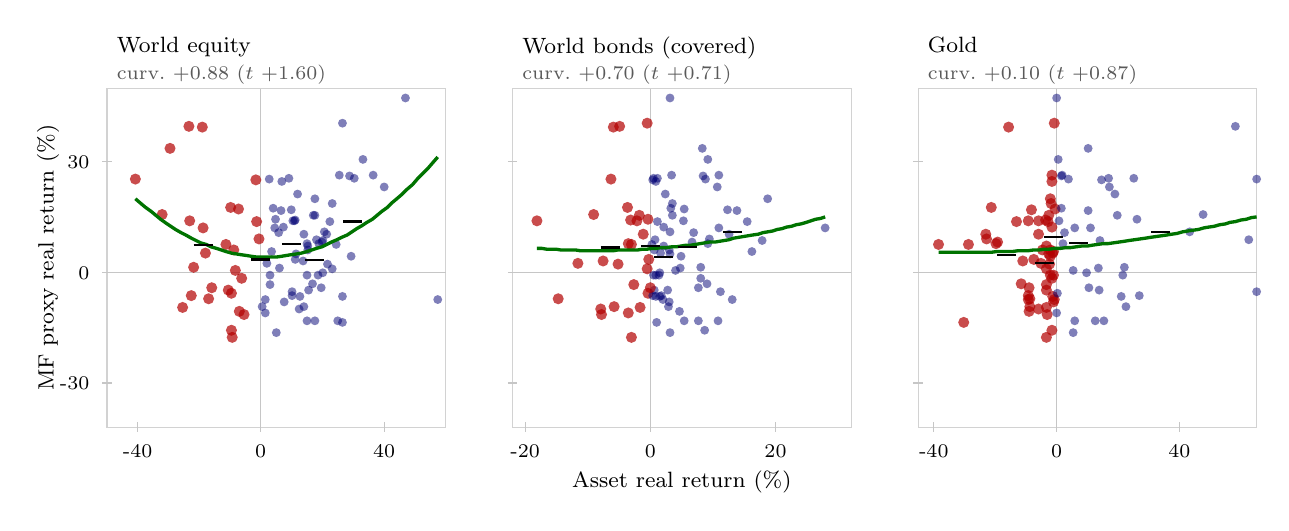
\begin{tikzpicture}[x=1cm, y=1cm]
  \draw[gray!35] (0.00,0) rectangle (4.30,4.30);
  \draw[gray!45] (0.00,1.96) -- (4.30,1.96);
  \draw[gray!45] (1.95,0) -- (1.95,4.30);
  \draw[gray!45] (0.39,-0.06) -- (0.39,0.06);
  \node[below, font=\scriptsize] at (0.39,-0.1) {-40};
  \draw[gray!45] (1.95,-0.06) -- (1.95,0.06);
  \node[below, font=\scriptsize] at (1.95,-0.1) {0};
  \draw[gray!45] (3.52,-0.06) -- (3.52,0.06);
  \node[below, font=\scriptsize] at (3.52,-0.1) {40};
  \draw[gray!45] (-0.06,0.56) -- (0.06,0.56);
  \node[left, font=\scriptsize] at (-0.10,0.56) {-30};
  \draw[gray!45] (-0.06,1.96) -- (0.06,1.96);
  \node[left, font=\scriptsize] at (-0.10,1.96) {0};
  \draw[gray!45] (-0.06,3.37) -- (0.06,3.37);
  \node[left, font=\scriptsize] at (-0.10,3.37) {30};
  \fill[blue!45!black, opacity=0.5] (3.08,3.19) circle (1.6pt);
  \fill[blue!45!black, opacity=0.5] (3.25,3.40) circle (1.6pt);
  \fill[red!70!black, opacity=0.7] (1.67,2.77) circle (2.0pt);
  \fill[red!70!black, opacity=0.7] (1.22,2.53) circle (2.0pt);
  \fill[red!70!black, opacity=0.7] (0.80,3.54) circle (2.0pt);
  \fill[blue!45!black, opacity=0.5] (2.13,2.53) circle (1.6pt);
  \fill[blue!45!black, opacity=0.5] (4.20,1.62) circle (1.6pt);
  \fill[blue!45!black, opacity=0.5] (2.35,1.72) circle (1.6pt);
  \fill[blue!45!black, opacity=0.5] (2.86,2.01) circle (1.6pt);
  \fill[blue!45!black, opacity=0.5] (2.95,3.20) circle (1.6pt);
  \fill[red!70!black, opacity=0.7] (0.96,1.52) circle (2.0pt);
  \fill[blue!45!black, opacity=0.5] (2.18,2.47) circle (1.6pt);
  \fill[blue!45!black, opacity=0.5] (2.01,1.45) circle (1.6pt);
  \fill[red!70!black, opacity=0.7] (1.71,1.89) circle (2.0pt);
  \fill[blue!45!black, opacity=0.5] (2.01,1.62) circle (1.6pt);
  \fill[blue!45!black, opacity=0.5] (1.97,1.53) circle (1.6pt);
  \fill[blue!45!black, opacity=0.5] (2.39,2.63) circle (1.6pt);
  \fill[blue!45!black, opacity=0.5] (2.40,2.20) circle (1.6pt);
  \fill[blue!45!black, opacity=0.5] (2.64,2.69) circle (1.6pt);
  \fill[red!70!black, opacity=0.7] (1.21,3.81) circle (2.0pt);
  \fill[red!70!black, opacity=0.7] (1.29,1.63) circle (2.0pt);
  \fill[red!70!black, opacity=0.7] (1.74,1.43) circle (2.0pt);
  \fill[blue!45!black, opacity=0.5] (2.11,2.78) circle (1.6pt);
  \fill[blue!45!black, opacity=0.5] (2.79,2.45) circle (1.6pt);
  \fill[blue!45!black, opacity=0.5] (2.44,1.50) circle (1.6pt);
  \fill[blue!45!black, opacity=0.5] (2.45,1.66) circle (1.6pt);
  \fill[blue!45!black, opacity=0.5] (2.25,1.59) circle (1.6pt);
  \fill[blue!45!black, opacity=0.5] (3.79,4.18) circle (1.6pt);
  \fill[blue!45!black, opacity=0.5] (2.99,3.86) circle (1.6pt);
  \fill[blue!45!black, opacity=0.5] (2.07,1.81) circle (1.6pt);
  \fill[red!70!black, opacity=0.7] (1.59,1.14) circle (2.0pt);
  \fill[blue!45!black, opacity=0.5] (3.10,2.17) circle (1.6pt);
  \fill[blue!45!black, opacity=0.5] (2.86,2.84) circle (1.6pt);
  \fill[blue!45!black, opacity=0.5] (2.07,1.93) circle (1.6pt);
  \fill[blue!45!black, opacity=0.5] (2.68,1.93) circle (1.6pt);
  \fill[red!70!black, opacity=0.7] (1.58,1.23) circle (2.0pt);
  \fill[blue!45!black, opacity=0.5] (2.55,2.25) circle (1.6pt);
  \fill[blue!45!black, opacity=0.5] (2.22,3.12) circle (1.6pt);
  \fill[blue!45!black, opacity=0.5] (2.24,2.54) circle (1.6pt);
  \fill[red!70!black, opacity=0.7] (1.61,2.25) circle (2.0pt);
  \fill[blue!45!black, opacity=0.5] (2.55,2.30) circle (1.6pt);
  \fill[blue!45!black, opacity=0.5] (2.56,1.74) circle (1.6pt);
  \fill[red!70!black, opacity=0.7] (1.57,2.79) circle (2.0pt);
  \fill[red!70!black, opacity=0.7] (1.58,1.70) circle (2.0pt);
  \fill[blue!45!black, opacity=0.5] (2.64,1.35) circle (1.6pt);
  \fill[blue!45!black, opacity=0.5] (2.76,2.48) circle (1.6pt);
  \fill[red!70!black, opacity=0.7] (1.04,3.82) circle (2.0pt);
  \fill[red!70!black, opacity=0.7] (0.70,2.70) circle (2.0pt);
  \fill[blue!45!black, opacity=0.5] (2.99,1.33) circle (1.6pt);
  \fill[blue!45!black, opacity=0.5] (2.36,2.62) circle (1.6pt);
  \fill[red!70!black, opacity=0.7] (1.89,3.14) circle (2.0pt);
  \fill[blue!45!black, opacity=0.5] (2.31,3.16) circle (1.6pt);
  \fill[blue!45!black, opacity=0.5] (2.06,3.15) circle (1.6pt);
  \fill[blue!45!black, opacity=0.5] (2.54,2.33) circle (1.6pt);
  \fill[red!70!black, opacity=0.7] (1.51,2.32) circle (2.0pt);
  \fill[blue!45!black, opacity=0.5] (2.21,2.75) circle (1.6pt);
  \fill[blue!45!black, opacity=0.5] (2.69,2.33) circle (1.6pt);
  \fill[red!70!black, opacity=0.7] (1.93,2.39) circle (2.0pt);
  \fill[blue!45!black, opacity=0.5] (3.38,3.20) circle (1.6pt);
  \fill[blue!45!black, opacity=0.5] (3.52,3.05) circle (1.6pt);
  \fill[blue!45!black, opacity=0.5] (2.42,2.96) circle (1.6pt);
  \fill[blue!45!black, opacity=0.5] (2.73,2.35) circle (1.6pt);
  \fill[blue!45!black, opacity=0.5] (2.39,2.13) circle (1.6pt);
  \fill[red!70!black, opacity=0.7] (1.07,1.67) circle (2.0pt);
  \fill[blue!45!black, opacity=0.5] (2.61,1.82) circle (1.6pt);
  \fill[red!70!black, opacity=0.7] (1.68,1.47) circle (2.0pt);
  \fill[blue!45!black, opacity=0.5] (2.74,2.37) circle (1.6pt);
  \fill[blue!45!black, opacity=0.5] (2.03,2.08) circle (1.6pt);
  \fill[blue!45!black, opacity=0.5] (2.64,2.90) circle (1.6pt);
  \fill[blue!45!black, opacity=0.5] (2.34,2.76) circle (1.6pt);
  \fill[blue!45!black, opacity=0.5] (2.50,2.45) circle (1.6pt);
  \fill[blue!45!black, opacity=0.5] (2.83,2.61) circle (1.6pt);
  \fill[blue!45!black, opacity=0.5] (2.80,2.07) circle (1.6pt);
  \fill[red!70!black, opacity=0.7] (1.33,1.77) circle (2.0pt);
  \fill[red!70!black, opacity=0.7] (1.25,2.21) circle (2.0pt);
  \fill[red!70!black, opacity=0.7] (1.10,2.03) circle (2.0pt);
  \fill[blue!45!black, opacity=0.5] (3.14,3.16) circle (1.6pt);
  \fill[blue!45!black, opacity=0.5] (2.38,2.62) circle (1.6pt);
  \fill[blue!45!black, opacity=0.5] (2.19,2.02) circle (1.6pt);
  \fill[blue!45!black, opacity=0.5] (2.62,2.69) circle (1.6pt);
  \fill[blue!45!black, opacity=0.5] (2.14,2.64) circle (1.6pt);
  \fill[red!70!black, opacity=0.7] (0.36,3.15) circle (2.0pt);
  \fill[blue!45!black, opacity=0.5] (2.99,1.66) circle (1.6pt);
  \fill[blue!45!black, opacity=0.5] (2.35,1.67) circle (1.6pt);
  \fill[red!70!black, opacity=0.7] (1.63,1.99) circle (2.0pt);
  \fill[blue!45!black, opacity=0.5] (2.54,1.35) circle (1.6pt);
  \fill[blue!45!black, opacity=0.5] (2.91,2.32) circle (1.6pt);
  \fill[blue!45!black, opacity=0.5] (2.09,2.23) circle (1.6pt);
  \fill[red!70!black, opacity=0.7] (1.90,2.61) circle (2.0pt);
  \fill[blue!45!black, opacity=0.5] (2.15,1.20) circle (1.6pt);
  \fill[blue!45!black, opacity=0.5] (2.74,1.96) circle (1.6pt);
  \fill[red!70!black, opacity=0.7] (1.54,1.74) circle (2.0pt);
  \fill[blue!45!black, opacity=0.5] (2.93,1.35) circle (1.6pt);
  \fill[blue!45!black, opacity=0.5] (2.50,1.53) circle (1.6pt);
  \fill[blue!45!black, opacity=0.5] (2.49,2.11) circle (1.6pt);
  \fill[red!70!black, opacity=0.7] (1.05,2.62) circle (2.0pt);
  \fill[blue!45!black, opacity=0.5] (2.72,1.77) circle (1.6pt);
  \fill[blue!45!black, opacity=0.5] (2.54,1.93) circle (1.6pt);
  \fill[blue!45!black, opacity=0.5] (2.66,2.38) circle (1.6pt);
  \draw[very thick, green!45!black] plot coordinates {(0.36,2.90) (0.43,2.84) (0.49,2.79) (0.56,2.74) (0.62,2.69) (0.68,2.64) (0.75,2.59) (0.81,2.55) (0.87,2.51) (0.94,2.47) (1.00,2.44) (1.07,2.40) (1.13,2.37) (1.19,2.34) (1.26,2.32) (1.32,2.29) (1.39,2.27) (1.45,2.25) (1.51,2.23) (1.58,2.21) (1.64,2.20) (1.70,2.19) (1.77,2.18) (1.83,2.17) (1.90,2.16) (1.96,2.16) (2.02,2.16) (2.09,2.16) (2.15,2.16) (2.22,2.17) (2.28,2.18) (2.34,2.19) (2.41,2.20) (2.47,2.21) (2.54,2.23) (2.60,2.25) (2.66,2.27) (2.73,2.29) (2.79,2.32) (2.85,2.35) (2.92,2.38) (2.98,2.41) (3.05,2.44) (3.11,2.48) (3.17,2.52) (3.24,2.56) (3.30,2.60) (3.37,2.64) (3.43,2.69) (3.49,2.74) (3.56,2.79) (3.62,2.85) (3.68,2.90) (3.75,2.96) (3.81,3.02) (3.88,3.08) (3.94,3.15) (4.00,3.21) (4.07,3.28) (4.13,3.35) (4.20,3.43)};
  \draw[black, thick] (1.10,2.31) -- (1.34,2.31);
  \draw[black, thick] (1.83,2.13) -- (2.07,2.13);
  \draw[black, thick] (2.22,2.33) -- (2.46,2.33);
  \draw[black, thick] (2.51,2.12) -- (2.75,2.12);
  \draw[black, thick] (3.00,2.61) -- (3.24,2.61);
  \node[anchor=north west, font=\footnotesize] at (0.00,5.08) {World equity};
  \node[anchor=north west, font=\scriptsize, text=black!65] at (0.00,4.72) {curv.\ +0.88 ($t$ +1.60)};
  \draw[gray!35] (5.15,0) rectangle (9.45,4.30);
  \draw[gray!45] (5.15,1.96) -- (9.45,1.96);
  \draw[gray!45] (6.90,0) -- (6.90,4.30);
  \draw[gray!45] (5.31,-0.06) -- (5.31,0.06);
  \node[below, font=\scriptsize] at (5.31,-0.1) {-20};
  \draw[gray!45] (6.90,-0.06) -- (6.90,0.06);
  \node[below, font=\scriptsize] at (6.90,-0.1) {0};
  \draw[gray!45] (8.49,-0.06) -- (8.49,0.06);
  \node[below, font=\scriptsize] at (8.49,-0.1) {20};
  \draw[gray!45] (5.09,0.56) -- (5.21,0.56);
  \draw[gray!45] (5.09,1.96) -- (5.21,1.96);
  \draw[gray!45] (5.09,3.37) -- (5.21,3.37);
  \fill[blue!45!black, opacity=0.5] (7.57,3.19) circle (1.6pt);
  \fill[blue!45!black, opacity=0.5] (7.63,3.40) circle (1.6pt);
  \fill[blue!45!black, opacity=0.5] (7.33,2.77) circle (1.6pt);
  \fill[blue!45!black, opacity=0.5] (7.77,2.53) circle (1.6pt);
  \fill[blue!45!black, opacity=0.5] (7.56,3.54) circle (1.6pt);
  \fill[blue!45!black, opacity=0.5] (9.12,2.53) circle (1.6pt);
  \fill[blue!45!black, opacity=0.5] (7.94,1.62) circle (1.6pt);
  \fill[blue!45!black, opacity=0.5] (7.79,1.72) circle (1.6pt);
  \fill[red!70!black, opacity=0.7] (6.86,2.01) circle (2.0pt);
  \fill[blue!45!black, opacity=0.5] (7.17,3.20) circle (1.6pt);
  \fill[red!70!black, opacity=0.7] (6.77,1.52) circle (2.0pt);
  \fill[blue!45!black, opacity=0.5] (7.45,2.47) circle (1.6pt);
  \fill[red!70!black, opacity=0.7] (6.62,1.45) circle (2.0pt);
  \fill[blue!45!black, opacity=0.5] (7.54,1.89) circle (1.6pt);
  \fill[blue!45!black, opacity=0.5] (7.06,1.62) circle (1.6pt);
  \fill[red!70!black, opacity=0.7] (6.44,1.53) circle (2.0pt);
  \fill[red!70!black, opacity=0.7] (6.65,2.63) circle (2.0pt);
  \fill[blue!45!black, opacity=0.5] (7.15,2.20) circle (1.6pt);
  \fill[blue!45!black, opacity=0.5] (7.18,2.69) circle (1.6pt);
  \fill[red!70!black, opacity=0.7] (6.43,3.81) circle (2.0pt);
  \fill[red!70!black, opacity=0.7] (5.73,1.63) circle (2.0pt);
  \fill[red!70!black, opacity=0.7] (6.28,1.43) circle (2.0pt);
  \fill[blue!45!black, opacity=0.5] (7.16,2.78) circle (1.6pt);
  \fill[red!70!black, opacity=0.7] (6.81,2.45) circle (2.0pt);
  \fill[red!70!black, opacity=0.7] (6.27,1.50) circle (2.0pt);
  \fill[blue!45!black, opacity=0.5] (7.02,1.66) circle (1.6pt);
  \fill[blue!45!black, opacity=0.5] (7.14,1.59) circle (1.6pt);
  \fill[blue!45!black, opacity=0.5] (7.15,4.18) circle (1.6pt);
  \fill[red!70!black, opacity=0.7] (6.86,3.86) circle (2.0pt);
  \fill[red!70!black, opacity=0.7] (6.69,1.81) circle (2.0pt);
  \fill[red!70!black, opacity=0.7] (6.66,1.14) circle (2.0pt);
  \fill[blue!45!black, opacity=0.5] (7.29,2.17) circle (1.6pt);
  \fill[blue!45!black, opacity=0.5] (7.18,2.84) circle (1.6pt);
  \fill[blue!45!black, opacity=0.5] (7.01,1.93) circle (1.6pt);
  \fill[blue!45!black, opacity=0.5] (6.97,1.93) circle (1.6pt);
  \fill[blue!45!black, opacity=0.5] (7.59,1.23) circle (1.6pt);
  \fill[blue!45!black, opacity=0.5] (7.14,2.25) circle (1.6pt);
  \fill[blue!45!black, opacity=0.5] (6.97,3.12) circle (1.6pt);
  \fill[blue!45!black, opacity=0.5] (7.07,2.54) circle (1.6pt);
  \fill[blue!45!black, opacity=0.5] (6.95,2.25) circle (1.6pt);
  \fill[blue!45!black, opacity=0.5] (7.07,2.30) circle (1.6pt);
  \fill[blue!45!black, opacity=0.5] (7.12,1.74) circle (1.6pt);
  \fill[red!70!black, opacity=0.7] (6.61,2.79) circle (2.0pt);
  \fill[red!70!black, opacity=0.7] (6.87,1.70) circle (2.0pt);
  \fill[blue!45!black, opacity=0.5] (7.33,1.35) circle (1.6pt);
  \fill[blue!45!black, opacity=0.5] (7.15,2.48) circle (1.6pt);
  \fill[red!70!black, opacity=0.7] (6.51,3.82) circle (2.0pt);
  \fill[red!70!black, opacity=0.7] (6.18,2.70) circle (2.0pt);
  \fill[blue!45!black, opacity=0.5] (6.98,1.33) circle (1.6pt);
  \fill[red!70!black, opacity=0.7] (6.73,2.62) circle (2.0pt);
  \fill[blue!45!black, opacity=0.5] (6.93,3.14) circle (1.6pt);
  \fill[blue!45!black, opacity=0.5] (6.99,3.16) circle (1.6pt);
  \fill[red!70!black, opacity=0.7] (6.40,3.15) circle (2.0pt);
  \fill[red!70!black, opacity=0.7] (6.62,2.33) circle (2.0pt);
  \fill[blue!45!black, opacity=0.5] (6.92,2.32) circle (1.6pt);
  \fill[blue!45!black, opacity=0.5] (8.00,2.75) circle (1.6pt);
  \fill[blue!45!black, opacity=0.5] (7.63,2.33) circle (1.6pt);
  \fill[blue!45!black, opacity=0.5] (7.65,2.39) circle (1.6pt);
  \fill[blue!45!black, opacity=0.5] (7.77,3.20) circle (1.6pt);
  \fill[blue!45!black, opacity=0.5] (7.75,3.05) circle (1.6pt);
  \fill[blue!45!black, opacity=0.5] (7.09,2.96) circle (1.6pt);
  \fill[blue!45!black, opacity=0.5] (7.43,2.35) circle (1.6pt);
  \fill[red!70!black, opacity=0.7] (6.88,2.13) circle (2.0pt);
  \fill[blue!45!black, opacity=0.5] (6.93,1.67) circle (1.6pt);
  \fill[blue!45!black, opacity=0.5] (7.62,1.82) circle (1.6pt);
  \fill[blue!45!black, opacity=0.5] (7.27,1.47) circle (1.6pt);
  \fill[blue!45!black, opacity=0.5] (8.32,2.37) circle (1.6pt);
  \fill[red!70!black, opacity=0.7] (5.98,2.08) circle (2.0pt);
  \fill[blue!45!black, opacity=0.5] (8.39,2.90) circle (1.6pt);
  \fill[blue!45!black, opacity=0.5] (7.88,2.76) circle (1.6pt);
  \fill[blue!45!black, opacity=0.5] (7.90,2.45) circle (1.6pt);
  \fill[blue!45!black, opacity=0.5] (8.13,2.61) circle (1.6pt);
  \fill[red!70!black, opacity=0.7] (6.49,2.07) circle (2.0pt);
  \fill[blue!45!black, opacity=0.5] (7.51,1.77) circle (1.6pt);
  \fill[blue!45!black, opacity=0.5] (7.03,2.21) circle (1.6pt);
  \fill[blue!45!black, opacity=0.5] (7.54,2.03) circle (1.6pt);
  \fill[blue!45!black, opacity=0.5] (6.94,3.16) circle (1.6pt);
  \fill[blue!45!black, opacity=0.5] (7.32,2.62) circle (1.6pt);
  \fill[blue!45!black, opacity=0.5] (7.28,2.02) circle (1.6pt);
  \fill[red!70!black, opacity=0.7] (6.76,2.69) circle (2.0pt);
  \fill[red!70!black, opacity=0.7] (6.87,2.64) circle (2.0pt);
  \fill[blue!45!black, opacity=0.5] (7.60,3.15) circle (1.6pt);
  \fill[blue!45!black, opacity=0.5] (6.97,1.66) circle (1.6pt);
  \fill[blue!45!black, opacity=0.5] (7.04,1.67) circle (1.6pt);
  \fill[blue!45!black, opacity=0.5] (7.22,1.99) circle (1.6pt);
  \fill[blue!45!black, opacity=0.5] (7.76,1.35) circle (1.6pt);
  \fill[red!70!black, opacity=0.7] (6.66,2.32) circle (2.0pt);
  \fill[blue!45!black, opacity=0.5] (8.19,2.23) circle (1.6pt);
  \fill[blue!45!black, opacity=0.5] (6.99,2.61) circle (1.6pt);
  \fill[blue!45!black, opacity=0.5] (7.15,1.20) circle (1.6pt);
  \fill[blue!45!black, opacity=0.5] (7.02,1.96) circle (1.6pt);
  \fill[blue!45!black, opacity=0.5] (6.95,1.74) circle (1.6pt);
  \fill[blue!45!black, opacity=0.5] (7.51,1.35) circle (1.6pt);
  \fill[blue!45!black, opacity=0.5] (7.13,1.53) circle (1.6pt);
  \fill[red!70!black, opacity=0.7] (6.30,2.11) circle (2.0pt);
  \fill[red!70!black, opacity=0.7] (5.46,2.62) circle (2.0pt);
  \fill[red!70!black, opacity=0.7] (6.90,1.77) circle (2.0pt);
  \fill[blue!45!black, opacity=0.5] (6.94,1.93) circle (1.6pt);
  \fill[blue!45!black, opacity=0.5] (6.96,2.38) circle (1.6pt);
  \draw[very thick, green!45!black] plot coordinates {(5.46,2.27) (5.52,2.27) (5.58,2.26) (5.64,2.26) (5.70,2.26) (5.76,2.25) (5.82,2.25) (5.88,2.25) (5.95,2.25) (6.01,2.24) (6.07,2.24) (6.13,2.24) (6.19,2.24) (6.25,2.24) (6.31,2.24) (6.37,2.24) (6.43,2.24) (6.49,2.25) (6.56,2.25) (6.62,2.25) (6.68,2.25) (6.74,2.25) (6.80,2.26) (6.86,2.26) (6.92,2.27) (6.98,2.27) (7.04,2.28) (7.11,2.28) (7.17,2.29) (7.23,2.29) (7.29,2.30) (7.35,2.31) (7.41,2.31) (7.47,2.32) (7.53,2.33) (7.59,2.34) (7.65,2.35) (7.72,2.35) (7.78,2.36) (7.84,2.37) (7.90,2.38) (7.96,2.40) (8.02,2.41) (8.08,2.42) (8.14,2.43) (8.20,2.44) (8.27,2.45) (8.33,2.47) (8.39,2.48) (8.45,2.49) (8.51,2.51) (8.57,2.52) (8.63,2.54) (8.69,2.55) (8.75,2.57) (8.81,2.58) (8.88,2.60) (8.94,2.62) (9.00,2.64) (9.06,2.65) (9.12,2.67)};
  \draw[black, thick] (6.27,2.28) -- (6.51,2.28);
  \draw[black, thick] (6.78,2.30) -- (7.02,2.30);
  \draw[black, thick] (6.95,2.16) -- (7.19,2.16);
  \draw[black, thick] (7.25,2.29) -- (7.49,2.29);
  \draw[black, thick] (7.82,2.48) -- (8.06,2.48);
  \node[anchor=north west, font=\footnotesize] at (5.15,5.08) {World bonds (covered)};
  \node[anchor=north west, font=\scriptsize, text=black!65] at (5.15,4.72) {curv.\ +0.70 ($t$ +0.71)};
  \draw[gray!35] (10.30,0) rectangle (14.60,4.30);
  \draw[gray!45] (10.30,1.96) -- (14.60,1.96);
  \draw[gray!45] (12.06,0) -- (12.06,4.30);
  \draw[gray!45] (10.50,-0.06) -- (10.50,0.06);
  \node[below, font=\scriptsize] at (10.50,-0.1) {-40};
  \draw[gray!45] (12.06,-0.06) -- (12.06,0.06);
  \node[below, font=\scriptsize] at (12.06,-0.1) {0};
  \draw[gray!45] (13.62,-0.06) -- (13.62,0.06);
  \node[below, font=\scriptsize] at (13.62,-0.1) {40};
  \draw[gray!45] (10.24,0.56) -- (10.36,0.56);
  \draw[gray!45] (10.24,1.96) -- (10.36,1.96);
  \draw[gray!45] (10.24,3.37) -- (10.36,3.37);
  \fill[blue!45!black, opacity=0.5] (12.12,3.19) circle (1.6pt);
  \fill[blue!45!black, opacity=0.5] (12.08,3.40) circle (1.6pt);
  \fill[red!70!black, opacity=0.7] (12.04,2.77) circle (2.0pt);
  \fill[blue!45!black, opacity=0.5] (12.29,2.53) circle (1.6pt);
  \fill[blue!45!black, opacity=0.5] (12.46,3.54) circle (1.6pt);
  \fill[blue!45!black, opacity=0.5] (12.49,2.53) circle (1.6pt);
  \fill[red!70!black, opacity=0.7] (12.03,1.62) circle (2.0pt);
  \fill[blue!45!black, opacity=0.5] (14.60,1.72) circle (1.6pt);
  \fill[red!70!black, opacity=0.7] (11.93,2.01) circle (2.0pt);
  \fill[red!70!black, opacity=0.7] (12.00,3.20) circle (2.0pt);
  \fill[red!70!black, opacity=0.7] (11.93,1.52) circle (2.0pt);
  \fill[blue!45!black, opacity=0.5] (12.16,2.47) circle (1.6pt);
  \fill[blue!45!black, opacity=0.5] (12.06,1.45) circle (1.6pt);
  \fill[red!70!black, opacity=0.7] (12.00,1.89) circle (2.0pt);
  \fill[red!70!black, opacity=0.7] (11.70,1.62) circle (2.0pt);
  \fill[red!70!black, opacity=0.7] (11.72,1.53) circle (2.0pt);
  \fill[red!70!black, opacity=0.7] (11.92,2.63) circle (2.0pt);
  \fill[red!70!black, opacity=0.7] (11.96,2.20) circle (2.0pt);
  \fill[red!70!black, opacity=0.7] (11.96,2.69) circle (2.0pt);
  \fill[red!70!black, opacity=0.7] (11.45,3.81) circle (2.0pt);
  \fill[red!70!black, opacity=0.7] (11.72,1.63) circle (2.0pt);
  \fill[red!70!black, opacity=0.7] (11.94,1.43) circle (2.0pt);
  \fill[blue!45!black, opacity=0.5] (12.12,2.78) circle (1.6pt);
  \fill[red!70!black, opacity=0.7] (11.83,2.45) circle (2.0pt);
  \fill[red!70!black, opacity=0.7] (11.83,1.50) circle (2.0pt);
  \fill[red!70!black, opacity=0.7] (12.01,1.66) circle (2.0pt);
  \fill[red!70!black, opacity=0.7] (12.02,1.59) circle (2.0pt);
  \fill[blue!45!black, opacity=0.5] (12.06,4.18) circle (1.6pt);
  \fill[red!70!black, opacity=0.7] (12.03,3.86) circle (2.0pt);
  \fill[red!70!black, opacity=0.7] (11.93,1.81) circle (2.0pt);
  \fill[red!70!black, opacity=0.7] (11.93,1.14) circle (2.0pt);
  \fill[red!70!black, opacity=0.7] (11.98,2.17) circle (2.0pt);
  \fill[red!70!black, opacity=0.7] (11.99,2.84) circle (2.0pt);
  \fill[red!70!black, opacity=0.7] (11.98,1.93) circle (2.0pt);
  \fill[red!70!black, opacity=0.7] (12.02,1.93) circle (2.0pt);
  \fill[red!70!black, opacity=0.7] (12.00,1.23) circle (2.0pt);
  \fill[red!70!black, opacity=0.7] (11.98,2.25) circle (2.0pt);
  \fill[red!70!black, opacity=0.7] (12.00,3.12) circle (2.0pt);
  \fill[red!70!black, opacity=0.7] (12.00,2.54) circle (2.0pt);
  \fill[red!70!black, opacity=0.7] (11.88,2.25) circle (2.0pt);
  \fill[red!70!black, opacity=0.7] (11.93,2.30) circle (2.0pt);
  \fill[blue!45!black, opacity=0.5] (12.60,1.74) circle (1.6pt);
  \fill[red!70!black, opacity=0.7] (11.23,2.79) circle (2.0pt);
  \fill[blue!45!black, opacity=0.5] (12.07,1.70) circle (1.6pt);
  \fill[blue!45!black, opacity=0.5] (12.55,1.35) circle (1.6pt);
  \fill[blue!45!black, opacity=0.5] (13.75,2.48) circle (1.6pt);
  \fill[blue!45!black, opacity=0.5] (14.33,3.82) circle (1.6pt);
  \fill[blue!45!black, opacity=0.5] (13.92,2.70) circle (1.6pt);
  \fill[red!70!black, opacity=0.7] (10.88,1.33) circle (2.0pt);
  \fill[red!70!black, opacity=0.7] (11.70,2.62) circle (2.0pt);
  \fill[blue!45!black, opacity=0.5] (12.63,3.14) circle (1.6pt);
  \fill[blue!45!black, opacity=0.5] (13.04,3.16) circle (1.6pt);
  \fill[blue!45!black, opacity=0.5] (14.60,3.15) circle (1.6pt);
  \fill[blue!45!black, opacity=0.5] (12.14,2.33) circle (1.6pt);
  \fill[red!70!black, opacity=0.7] (10.56,2.32) circle (2.0pt);
  \fill[blue!45!black, opacity=0.5] (12.46,2.75) circle (1.6pt);
  \fill[red!70!black, opacity=0.7] (11.29,2.33) circle (2.0pt);
  \fill[red!70!black, opacity=0.7] (11.17,2.39) circle (2.0pt);
  \fill[blue!45!black, opacity=0.5] (12.13,3.20) circle (1.6pt);
  \fill[blue!45!black, opacity=0.5] (12.73,3.05) circle (1.6pt);
  \fill[blue!45!black, opacity=0.5] (12.80,2.96) circle (1.6pt);
  \fill[red!70!black, opacity=0.7] (11.31,2.35) circle (2.0pt);
  \fill[red!70!black, opacity=0.7] (11.77,2.13) circle (2.0pt);
  \fill[red!70!black, opacity=0.7] (11.70,1.67) circle (2.0pt);
  \fill[red!70!black, opacity=0.7] (11.61,1.82) circle (2.0pt);
  \fill[red!70!black, opacity=0.7] (11.71,1.47) circle (2.0pt);
  \fill[blue!45!black, opacity=0.5] (12.61,2.37) circle (1.6pt);
  \fill[red!70!black, opacity=0.7] (11.86,2.08) circle (2.0pt);
  \fill[red!70!black, opacity=0.7] (11.98,2.90) circle (2.0pt);
  \fill[red!70!black, opacity=0.7] (11.74,2.76) circle (2.0pt);
  \fill[red!70!black, opacity=0.7] (11.16,2.45) circle (2.0pt);
  \fill[red!70!black, opacity=0.7] (11.95,2.61) circle (2.0pt);
  \fill[red!70!black, opacity=0.7] (11.97,2.07) circle (2.0pt);
  \fill[red!70!black, opacity=0.7] (11.71,1.77) circle (2.0pt);
  \fill[red!70!black, opacity=0.7] (12.01,2.21) circle (2.0pt);
  \fill[blue!45!black, opacity=0.5] (12.92,2.03) circle (1.6pt);
  \fill[blue!45!black, opacity=0.5] (12.72,3.16) circle (1.6pt);
  \fill[blue!45!black, opacity=0.5] (12.09,2.62) circle (1.6pt);
  \fill[blue!45!black, opacity=0.5] (12.59,2.02) circle (1.6pt);
  \fill[blue!45!black, opacity=0.5] (12.83,2.69) circle (1.6pt);
  \fill[blue!45!black, opacity=0.5] (13.08,2.64) circle (1.6pt);
  \fill[blue!45!black, opacity=0.5] (12.21,3.15) circle (1.6pt);
  \fill[blue!45!black, opacity=0.5] (12.88,1.66) circle (1.6pt);
  \fill[blue!45!black, opacity=0.5] (13.11,1.67) circle (1.6pt);
  \fill[blue!45!black, opacity=0.5] (12.27,1.99) circle (1.6pt);
  \fill[blue!45!black, opacity=0.5] (12.29,1.35) circle (1.6pt);
  \fill[red!70!black, opacity=0.7] (10.94,2.32) circle (2.0pt);
  \fill[red!70!black, opacity=0.7] (12.02,2.23) circle (2.0pt);
  \fill[red!70!black, opacity=0.7] (11.55,2.61) circle (2.0pt);
  \fill[blue!45!black, opacity=0.5] (12.27,1.20) circle (1.6pt);
  \fill[blue!45!black, opacity=0.5] (12.44,1.96) circle (1.6pt);
  \fill[red!70!black, opacity=0.7] (11.93,1.74) circle (2.0pt);
  \fill[blue!45!black, opacity=0.5] (12.66,1.35) circle (1.6pt);
  \fill[blue!45!black, opacity=0.5] (12.94,1.53) circle (1.6pt);
  \fill[red!70!black, opacity=0.7] (11.63,2.11) circle (2.0pt);
  \fill[red!70!black, opacity=0.7] (11.83,2.62) circle (2.0pt);
  \fill[blue!45!black, opacity=0.5] (12.47,1.77) circle (1.6pt);
  \fill[blue!45!black, opacity=0.5] (12.90,1.93) circle (1.6pt);
  \fill[blue!45!black, opacity=0.5] (14.50,2.38) circle (1.6pt);
  \draw[very thick, green!45!black] plot coordinates {(10.56,2.22) (10.63,2.22) (10.69,2.22) (10.76,2.22) (10.83,2.22) (10.90,2.22) (10.96,2.22) (11.03,2.22) (11.10,2.22) (11.17,2.22) (11.23,2.22) (11.30,2.23) (11.37,2.23) (11.43,2.23) (11.50,2.23) (11.57,2.24) (11.64,2.24) (11.70,2.24) (11.77,2.25) (11.84,2.25) (11.91,2.26) (11.97,2.26) (12.04,2.27) (12.11,2.27) (12.18,2.28) (12.24,2.28) (12.31,2.29) (12.38,2.30) (12.45,2.30) (12.51,2.31) (12.58,2.32) (12.65,2.33) (12.71,2.33) (12.78,2.34) (12.85,2.35) (12.92,2.36) (12.98,2.37) (13.05,2.38) (13.12,2.39) (13.19,2.40) (13.25,2.41) (13.32,2.42) (13.39,2.43) (13.46,2.44) (13.52,2.45) (13.59,2.46) (13.66,2.48) (13.72,2.49) (13.79,2.50) (13.86,2.51) (13.93,2.53) (13.99,2.54) (14.06,2.55) (14.13,2.57) (14.20,2.58) (14.26,2.60) (14.33,2.61) (14.40,2.63) (14.47,2.64) (14.53,2.66) (14.60,2.67)};
  \draw[black, thick] (11.30,2.19) -- (11.54,2.19);
  \draw[black, thick] (11.79,2.08) -- (12.03,2.08);
  \draw[black, thick] (11.90,2.41) -- (12.14,2.41);
  \draw[black, thick] (12.22,2.34) -- (12.46,2.34);
  \draw[black, thick] (13.26,2.48) -- (13.50,2.48);
  \node[anchor=north west, font=\footnotesize] at (10.30,5.08) {Gold};
  \node[anchor=north west, font=\scriptsize, text=black!65] at (10.30,4.72) {curv.\ +0.10 ($t$ +0.87)};
  \node[font=\footnotesize] at (7.30,-0.7) {Asset real return (\%)};
  \node[rotate=90, font=\footnotesize] at (-0.75,2.15) {MF proxy real return (\%)};
\end{tikzpicture}

\caption{Annual real return of the net managed-futures proxy against the annual
real return of each asset class, U.S.\ resident, 1927--2025. Each point is one
year, with red points the years the asset itself lost and blue points the years
it gained. The green curve is a descriptive quadratic fit and the black ticks
are the mean proxy return within each quintile of the asset's return. ``curv.''
is the coefficient on the squared term, and $t$ is its
heteroskedasticity-robust (White HC1) statistic.}
\label{fig:mf-convexity}
\end{figure}

The bottom panel of Table~\ref{tab:mf-diagnostics} takes the ten worst years for
world equity and reads off the proxy. It is positive in eight of them, sharply
so in the persistent bear markets, with $+34\%$ in 1931, $+40\%$ in 1946 and
1973, and $+25\%$ in 2008, because a trend rule has time to establish short
positions while prices fall through the year. The two misses, 1937 ($-10\%$) and
1990 ($-6\%$), are fast reversals where the signal is still long when the market
turns, and 2002 ($+1\%$) is roughly flat. This is convex behavior earned by
directionality, not a static short or a volatility position, and it is the same
property that makes the sleeve lower retirement ruin in the main results. The
proxy is not, however, a dedicated inflation hedge. Across the highest-inflation
years it wins the drawn-out episodes (1974, 1979, 2022) and loses the
single-year spikes (1942, 1947, 1951), and its correlation with inflation is
only mildly negative.

Two construction caveats carry over from Section~\ref{sec:data}. The pre-1960
segment rests on a thin market set, which inflates the proxy's early realized
volatility without raising its mean and drives the pre-1970 weakness of the
levered portfolios in Section~\ref{sec:subperiods}. And the series is a
reconstruction from public price data, not an investable index net of the full
implementation cost a fund would incur.

\subsection{Sensitivity to the construction choices}
\label{app:mf-variants}

The baseline proxy blends one-, six-, and twelve-month momentum signals and
charges a 0.85\% management fee plus a measured turnover cost. To show the
results do not turn on that specific recipe,
Table~\ref{tab:mf-variants} rebuilds the annual real series four other ways,
using the identical volatility target, sector weighting, and month-by-month
deflation, and each variant carrying its own realized turnover cost. The
one-, three-, and twelve-month blend of \citet{HurstOoiPedersen2017} correlates
0.96 with the baseline. The twelve-month signal alone, the original
specification of \citet{MoskowitzOoiPedersen2012}, has the same mean and
volatility and correlates 0.83, differing mainly in a lower skew. Even the
one-month signal alone, the fastest and worst-performing variant, correlates
0.77. Doubling the management fee to 1.70\% shifts the mean down by the
fee difference and leaves the return path, and therefore the correlation,
unchanged.

A high correlation is reassuring but not decisive, because retirement ruin and
the equivalent saving depend on the order of returns in the worst bootstrap
sequences, not on the full-sample correlation alone. Table~\ref{tab:mf-variant-lifecycle}
therefore reruns the entire lifecycle model with each variant's gross signal
series in the sleeve, for the two 200\% families, at the same seed and 10,000
paired paths as the main tables.

The design isolates the signal, not the cost. Every row applies the same flat
turnover drag as the baseline, so the lifecycle comparison holds cost constant
and varies only the signal specification. The faster signals would in reality
bear higher realized turnover; Table~\ref{tab:mf-variants} reports each
variant's own measured turnover cost at the series level.

The outcome is uniform. Every variant row sits well below the ACO line on both
criteria: ruin between 1.7\% and 3.0\% against ACO's 7.36\%, and
equivalent saving between 5.2\% and 7.6\% against ACO's 10\%. The
weakest case is the one-month signal, the roughest and lowest-Sharpe
alternative, with 2.11\% and 2.85\% ruin and 5.96\% and 7.57\% saving.
Doubling the fee to 1.70\% raises the required saving by about 0.5 to
0.8 point and leaves ruin near the baseline. The diversification result
therefore does not hinge on the signal blend, and the cost dimension is
bounded separately by the fee row and by each variant's measured turnover in
Table~\ref{tab:mf-variants}.

\begin{table}[H]
\centering
\caption{Managed-futures proxy under alternative construction choices}
\label{tab:mf-variants}
\small
% Genere par build/mf_variants.py -- ne pas editer.
\begin{tabular}{lrrrrrr}
\toprule
Variant & Mean & SD & Sharpe$_0$ & Skew & 5th pctl & Corr.\ baseline \\
\midrule
1/6/12 blend (baseline)$^{\dagger}$ & 7.91\% & 13.98\% & 0.57 & +0.45 & -11.8\% & 1.000 \\
1/3/12 blend & 7.94\% & 14.21\% & 0.56 & +0.66 & -11.2\% & 0.957 \\
12-month signal only & 8.19\% & 14.58\% & 0.56 & +0.21 & -14.3\% & 0.831 \\
1-month signal only & 5.57\% & 12.53\% & 0.44 & +0.61 & -10.6\% & 0.759 \\
1/6/12 blend, fee doubled to 1.70\% & 6.98\% & 13.86\% & 0.50 & +0.45 & -12.6\% & 1.000 \\
\bottomrule
\end{tabular}

\begin{minipage}{0.94\textwidth}\footnotesize
\textit{Note:} U.S.\ resident, annual real returns, 1927--2025, net of each
variant's management fee and its own realized turnover cost. ``Corr.\
baseline'' is the Pearson correlation of the annual series with the
$1/6/12$ blend used throughout the paper. The baseline mean here differs from
Table~\ref{tab:mf-diagnostics} by about 0.15 point because that table applies
a flat annual turnover drag while this one compounds the monthly realized cost.
The correlations are unaffected by the cost convention. $^{\dagger}$Baseline.
\end{minipage}
\end{table}

\begin{table}[H]
\centering
\caption{Lifecycle outcomes with each managed-futures variant in the sleeve}
\label{tab:mf-variant-lifecycle}
\small
% Genere par build/mf_variant_lifecycle.py -- ne pas editer.
\begin{tabular}{lrrrrr}
\toprule
MF sleeve & Corr.\ & \multicolumn{2}{c}{Proportional 200\%} & \multicolumn{2}{c}{Equal-weight 200\%} \\
\cmidrule(lr){3-4}\cmidrule(lr){5-6}
 & baseline & Ruin & Equiv.\ saving & Ruin & Equiv.\ saving \\
\midrule
\emph{ACO 33/67 (all-equity)} & --- & \emph{7.36\%} & \emph{10.00\%} & \emph{7.36\%} & \emph{10.00\%} \\
\addlinespace
\quad 1/6/12 blend (baseline)$^{\dagger}$ & 1.00 & 1.83\% & 5.32\% & 2.51\% & 6.40\% \\
\quad 1/3/12 blend & 0.96 & 1.72\% & 5.24\% & 2.48\% & 6.25\% \\
\quad 12-month signal only & 0.83 & 2.00\% & 5.53\% & 2.92\% & 6.76\% \\
\quad 1-month signal only & 0.77 & 2.11\% & 5.96\% & 2.85\% & 7.57\% \\
\quad 1/6/12 blend, fee doubled to 1.70\% & 1.00 & 2.08\% & 5.77\% & 2.98\% & 7.24\% \\
\bottomrule
\end{tabular}

\begin{minipage}{0.94\textwidth}\footnotesize
\textit{Note:} Each row rebuilds the country-year panel with the variant's
U.S.\ gross annual real series in the managed-futures column, covers it into
each resident's currency by the same rule as the paper's panel, and evaluates
the two 200\% families and the ACO 33/67 benchmark on 10,000 paired
lifecycle paths at seed 20260827. Entries are levels, in percent: retirement
ruin and the utility-equivalent saving rate, both lower is better. The ACO
33/67 all-equity line is shown first for reference. The model applies its flat
turnover drag identically across variants, so the table is a
signal-specification sensitivity at constant cost rather than an
implementation test. The signal-specific turnover costs of
Table~\ref{tab:mf-variants} enter only there. The baseline row
reproduces the 200\% rows of Table~\ref{tab:main-ladders} exactly.
$^{\dagger}$Baseline.
\end{minipage}
\end{table}

\section{Gold availability before 1968}
\label{app:gold-availability}

The standard results use the spliced historical gold-price series throughout.
Before 1968, however, that price was administered and does not represent an
ordinary investable gold sleeve. We therefore run a separate availability
exercise. Whenever a bootstrap draw precedes 1968, the portfolio's gold
notional is allocated equally among its already active non-gold sleeves. Thus,
for example, the 20\% gold sleeve of 54/36/20/20 becomes 6.67 percentage points
each of ACO equity, covered bonds, and managed futures, while gross exposure,
financing, and all post-1967 gold returns are unchanged.

\begin{table}[H]
\centering
\caption{Gold-availability rule before 1968}
\label{tab:gold-availability}
\begin{tabular}{lrrrr}
\toprule
& \multicolumn{2}{c}{Raw gold-price series}
& \multicolumn{2}{c}{Gold unavailable before 1968} \\
Portfolio & Saving & Ruin & Saving & Ruin \\
\midrule
60/40 ACO $+$ 33.33 gold & 11.00\% & 4.38\% & 9.42\% & 3.11\% \\
54/36/20/20 ACO & 9.76 & 3.19 & 8.90 & 2.55 \\
90/60/25/25 ACO & 5.36 & 1.96 & 4.79 & 1.65 \\
\bottomrule
\end{tabular}
\begin{minipage}{0.96\textwidth}\footnotesize
\textit{Note:} 10,000 paired simulations. ``Gold unavailable'' is not an
assumed gold return. Before 1968, the gold exposure is redistributed in equal
dollar amounts across the non-gold sleeves already held by that recipe. Total
gross exposure and the financing position are unchanged. Saving is
utility-equivalent saving relative to ACO 33/67 at 10\%.
\end{minipage}
\end{table}

The improvement shows that the administered-price segment materially affects
the raw gold comparison. It does not identify the return that freely tradeable
gold would have earned before 1968, nor does it establish a standalone gold
premium. It evaluates the more realistic decision rule of not holding that
sleeve when it was unavailable.

\section{Leverage ladders}
\label{app:leverage-ladders}

Sections~\ref{sec:leverage-ladders-main} and~\ref{sec:comparable-risk} report
the ladder results in the main text. This appendix retains the detailed
weight-by-weight tables as an audit trail. All of them use the same
1{,}557-country-year raw panel, block bootstrap, and paired benchmark; the
frontier runs on 5{,}000 paths and the complete ladders on 10{,}000. Two
reading notes make the alternative presentations consistent with one another.

The first note concerns the leverage frontier of Table~\ref{tab:frontier}. Its
``90/60 covered bonds'' column sweeps a leverage multiplier, so each row is
the 60/40 mix scaled up to the gross exposure in the margin. The match with
Table~\ref{tab:lifecycle} is made on gross exposure. At 100\% gross the
frontier row is an \emph{unlevered} 60/40, and it sits $+1.4$ points above the
benchmark only because it takes less risk, not because it is a better
portfolio at equal risk. At 150\% gross the frontier row \emph{is}
Table~\ref{tab:lifecycle}'s 90/60 covered, and the two runs agree: the ruin
gap against the benchmark reads $+0.4$ point in the frontier against $+0.45$
in Table~\ref{tab:lifecycle}, the same quantity within Monte Carlo error.
Across the ladder the covered 90/60's gap traces a shallow U within about a
point of zero.

The second note concerns the two ladder tables below, which give the exact row
definitions underlying the two main-text families. The gross-exposure levels
are set directly in the manifest, and realized volatility is reported only
after evaluation---the weights are never chosen to hit a volatility target.

\begin{table}[H]
\centering
\caption{Proportional 60/40/25/25 leverage ladder}
\label{tab:60402525-ladder}
\small
\begin{tabular}{rlrrr}
\toprule
Gross & Equity/Bonds/Gold/MF & Volatility & Saving & Ruin \\
\midrule
100\% & 40/26.67/16.67/16.67 & 10.00\% & 13.17\% & 4.87\% \\
125\% & 50/33.33/20.83/20.83 & 11.82 & 10.25 & 3.32 \\
150\% & 60/40/25/25 & 13.75 & 8.13 & 2.47 \\
175\% & 70/46.67/29.17/29.17 & 15.75 & 6.54 & 2.06 \\
200\% & 80/53.33/33.33/33.33 & 17.80 & 5.32 & 1.83 \\
\bottomrule
\end{tabular}
\begin{minipage}{0.96\textwidth}\footnotesize
\textit{Note:} Each row is a proportional scaling of the 150\% 60/40/25/25
anchor. Equity is the ACO 33/67 sleeve, and bonds and managed futures are
covered. Saving is utility-equivalent saving. The weights are fixed before
computing the reported realized volatility.
\end{minipage}
\end{table}

\begin{table}[H]
\centering
\caption{Equal-weight four-sleeve leverage ladder}
\label{tab:equal-ladder}
\begin{tabular}{rrrrr}
\toprule
Gross exposure & Each sleeve & Volatility & Saving & Ruin \\
\midrule
100\% & 25.00\% & 9.68\% & 14.54\% & 5.79\% \\
125\% & 31.25 & 11.38 & 11.57 & 4.10 \\
150\% & 37.50 & 13.19 & 9.36 & 3.27 \\
175\% & 43.75 & 15.08 & 7.70 & 2.64 \\
200\% & 50.00 & 17.02 & 6.40 & 2.51 \\
\bottomrule
\end{tabular}
\begin{minipage}{0.96\textwidth}\footnotesize
\textit{Note:} ``Each sleeve'' is ACO equity, covered world bonds, gold, and
managed futures. The five gross-exposure levels are fixed directly in the
manifest, and realized volatility is reported only after evaluation.
\end{minipage}
\end{table}

The comparable-volatility band that collects these ladder endpoints with the
90/60 controls is Table~\ref{tab:main-similar-volatility} in the main text. The
volatility there is the pooled one-year-return standard deviation of
Table~\ref{tab:moments}, not the retirement-path volatility of
Table~\ref{tab:frontier}.

\section{Historical-sample uncertainty}
\label{app:historical-uncertainty}

The main simulation's Monte Carlo intervals answer a narrow numerical question:
how precisely does a fixed empirical distribution map into simulated lifecycle
outcomes? They leave open the more substantive question of whether the observed
1927--2025, sixteen-country history is unusually favorable to the diversified
families. We therefore perturb the historical input in four transparent ways:
we shorten and lengthen stationary blocks from ten to five and twenty years,
start the available history in 1950 and 1970, apply the ex ante investability
screen of Section~\ref{sec:data}, and omit each country in turn. The
strategies, their 200\% gross exposures, all fees, and the 0.30\% financing
spread remain fixed. No weights, leverage, or asset universe is re-selected in
any row.

Table~\ref{tab:historical-uncertainty} reports the two lifecycle quantities on
which the central conclusion rests, as levels: retirement ruin and the
utility-equivalent saving rate for each family, next to the ACO 33/67 ruin
column, with ACO's equivalent saving fixed at 10\%. Lower is better in every
column. The leave-one-country-out minimum, median, and maximum are reported
cell by cell, and the full country-level audit is
Table~\ref{tab:historical-uncertainty-loo}. These are deliberately not
labeled confidence intervals. The windows overlap, countries are not
independent draws, and the dates 1950 and 1970 are economically motivated
stress tests rather than a random design.

\begin{table}[H]
\centering
\caption{Historical-sample sensitivity of the fixed diversified families}
\label{tab:historical-uncertainty}
\scriptsize\setlength{\tabcolsep}{3pt}
\begin{tabular}{lrrrrrr}
\toprule
Sample & $N$ & ACO ruin & \multicolumn{2}{c}{Proportional 200\%} & \multicolumn{2}{c}{Equal-weight 200\%} \\
\cmidrule(lr){4-5}\cmidrule(lr){6-7}
 & & & Ruin & Equiv.\ saving & Ruin & Equiv.\ saving \\
\multicolumn{7}{l}{\emph{lower is better, ACO equivalent saving is $10\%$ throughout}} \\
\midrule
Full panel{,} 5-year blocks & 1{,}557 & \emph{8.88\%} & 2.68\% & 5.34\% & 3.18\% & 6.43\% \\
Full panel{,} 10-year blocks & 1{,}557 & \emph{6.96\%} & 1.94\% & 5.33\% & 2.76\% & 6.40\% \\
Full panel{,} 20-year blocks & 1{,}557 & \emph{6.40\%} & 1.32\% & 5.45\% & 1.74\% & 6.57\% \\
1950--2025{,} 10-year blocks & 1{,}213 & \emph{5.88\%} & 0.38\% & 4.89\% & 0.62\% & 5.66\% \\
1970--2025{,} 10-year blocks & 894 & \emph{4.52\%} & 0.20\% & 4.16\% & 0.22\% & 4.90\% \\
Investability screen{,} 10-year blocks & 1{,}527 & \emph{5.16\%} & 0.46\% & 5.30\% & 0.72\% & 6.28\% \\
LOO minimum (16 countries) & 1{,}458--1{,}466 & \emph{6.28\%} & 1.22\% & 5.30\% & 1.80\% & 6.33\% \\
LOO median (16 countries) & 1{,}458--1{,}466 & \emph{7.46\%} & 2.02\% & 5.42\% & 2.68\% & 6.52\% \\
LOO maximum (16 countries) & 1{,}458--1{,}466 & \emph{8.16\%} & 2.22\% & 5.54\% & 2.88\% & 6.70\% \\
\bottomrule
\end{tabular}
\begin{minipage}{0.97\textwidth}\footnotesize
\textit{Note:} Each row uses 5{,}000 paired lifecycle paths. Entries are levels, in percent: retirement ruin and the utility-equivalent saving rate, both lower is better. The ACO 33/67 ruin column is the reference and its equivalent saving is $10\%$ throughout. The two 200\% families retain their fixed 200\% gross exposures, and no weight or leverage is re-estimated. ``LOO'' reports the cellwise minimum, median, and maximum across the sixteen leave-one-country-out samples, so a row need not correspond to one common omitted country. These are historical sensitivity results, not confidence intervals.
\end{minipage}
\end{table}


Every row keeps both families below the ACO line on both criteria. The
block-length and start-date perturbations move the levels but not the
ranking: across the five specifications, proportional ruin runs from 0.2\%
to 2.7\% against ACO's 4.5\% to 8.9\%, with equivalent saving of 4.2\% to
5.5\% against ACO's 10\%, and the equal-weight family runs from 0.2\% to
3.2\% ruin and 4.9\% to 6.6\% saving. The investability screen, which drops
30 country-years and leaves 1{,}527, tells the same story: ACO ruin is 5.16\%
against proportional 0.46\% and equal-weight 0.72\%, with equivalent saving
of 5.30\% and 6.28\%, so the documented screen changes the levels but not
the ranking. Leave-one-country-out is the sharpest of the four tests, because
it asks whether any single national history carries the result. It does not:
omitting any one country leaves proportional ruin between 1.2\% and 2.2\% and
equal-weight ruin between 1.8\% and 2.9\%, always below the matching ACO
figure, with equivalent saving between 5.3\% and 5.5\% for the proportional
family and between 6.3\% and 6.7\% for the equal-weight family. This audit
therefore increases confidence that the central ranking is not carried by a
single block convention, historical era, investability convention, or country.
It does not validate the long reconstructed sleeves outside the limits
documented elsewhere in this appendix.

The exercise is demanding of the claim. Shorter blocks reduce the persistence
of historical regimes and longer blocks increase it, late starts remove the
interwar and early postwar experience, and leave-one-out reveals whether a
single national history carries the result. Thus a sign reversal in this
appendix would be evidence against generality, not noise to average away. The
reported ranges should be read as the historical uncertainty remaining after
the ordinary paired Monte Carlo error has been made small.

\begin{table}[H]
\centering
\caption{Leave-one-country-out historical sensitivity}
\label{tab:historical-uncertainty-loo}
\small
\begin{tabular}{lrrrrr}
\toprule
Omitted country & ACO ruin & \multicolumn{2}{c}{Proportional 200\%} & \multicolumn{2}{c}{Equal-weight 200\%} \\
\cmidrule(lr){3-4}\cmidrule(lr){5-6}
 & & Ruin & Equiv.\ saving & Ruin & Equiv.\ saving \\
\multicolumn{6}{l}{\emph{lower is better, ACO equivalent saving is $10\%$}} \\
\midrule
Australia & \emph{7.44\%} & 2.16\% & 5.36\% & 2.86\% & 6.46\% \\
Belgium & \emph{7.46\%} & 1.60\% & 5.35\% & 2.10\% & 6.41\% \\
Denmark & \emph{8.16\%} & 1.82\% & 5.30\% & 2.26\% & 6.33\% \\
Finland & \emph{7.96\%} & 1.80\% & 5.34\% & 2.24\% & 6.34\% \\
France & \emph{7.04\%} & 2.10\% & 5.47\% & 2.50\% & 6.56\% \\
Germany & \emph{7.38\%} & 2.22\% & 5.43\% & 2.88\% & 6.53\% \\
Italy & \emph{6.82\%} & 1.96\% & 5.34\% & 2.64\% & 6.39\% \\
Japan & \emph{6.28\%} & 1.22\% & 5.43\% & 1.80\% & 6.66\% \\
Netherlands & \emph{7.46\%} & 1.90\% & 5.48\% & 2.68\% & 6.54\% \\
Norway & \emph{7.58\%} & 1.86\% & 5.47\% & 2.74\% & 6.52\% \\
Portugal & \emph{7.20\%} & 1.78\% & 5.54\% & 2.82\% & 6.66\% \\
Spain & \emph{8.04\%} & 2.08\% & 5.41\% & 2.58\% & 6.70\% \\
Sweden & \emph{7.84\%} & 2.08\% & 5.38\% & 2.68\% & 6.43\% \\
Switzerland & \emph{7.24\%} & 2.12\% & 5.45\% & 2.78\% & 6.55\% \\
UK & \emph{7.96\%} & 2.14\% & 5.41\% & 2.82\% & 6.48\% \\
USA & \emph{7.82\%} & 2.14\% & 5.44\% & 2.74\% & 6.54\% \\
\bottomrule
\end{tabular}
\begin{minipage}{0.94\textwidth}\footnotesize
\textit{Note:} 5{,}000 paired paths per omission, ten-year mean stationary blocks. Levels in percent, lower is better, with the same columns as Table~\ref{tab:historical-uncertainty}.
\end{minipage}
\end{table}


\section{Risk-aversion sensitivity}
\label{app:gamma-sensitivity}

Section~\ref{sec:benchmark} notes that ranking portfolios by expected lifecycle
utility, without holding the risk budget fixed, makes the ranking sensitive to
the risk each rule carries and to the coefficient of relative risk aversion
$\gamma$. ACO run the symmetric check on their side, varying $\gamma$ from
0.5 to 10 and reporting that the \emph{optimal} fixed weight stays near
one-third domestic equity with no bond allocation at any $\gamma$. They do not
report how the welfare magnitudes move. We apply the same test to our own
ranking. Here $\gamma$ is an exogenous household preference, not a quantity we
select or optimize over, and the exercise asks only whether the fixed
diversified rule keeps its advantage. We hold the two central families at their
fixed $200\%$ weights and gross exposure and vary $\gamma$ over $\{2, 3, 3.84,
5, 7.5, 10\}$, an empirically plausible subset of ACO's range, where $3.84$ is
the baseline and 7.5 is also the mean household estimate of
\citet{CalvetCampbellGomesSodini2025} that ACO cite. We do not go below
$\gamma=2$, for a mechanical rather than an economic reason. To reproduce
ACO's monthly bequest calibration at every risk aversion, the bequest
intensity is rescaled to each $\gamma$ as $\theta(\gamma) = \theta_{3.84}\cdot
12^{\,3.84-\gamma}$. This rescaling grows explosively as $\gamma$ falls toward
one, and at $\gamma\le 1$ the bequest term rather than the risk-aversion
coefficient itself would drive the utility comparison. Over
$\gamma\in[2,10]$ the rescaling still makes the bequest term economically
large at the low end and small at the high end, as in ACO's own grid.

Table~\ref{tab:gamma-sensitivity} reports the result as levels, with ACO's
ruin (7.36\%) and equivalent saving (10\%) as the reference. Retirement
ruin does not depend on $\gamma$ at all: it is a wealth-depletion event,
recorded before preferences enter, so the
proportional family holds at 1.83\% ruin and the equal-weight family at
2.51\% across the whole grid, both far below ACO's 7.36\%. The
utility-equivalent saving does respond to $\gamma$, but it never approaches
ACO's 10\%. The diversified edge is smallest near the baseline, where the
families need 5.32\% and 6.40\%, and widens as $\gamma$ moves away from it:
2.57\% and 3.74\% at $\gamma=2$, and 4.82\% and 5.98\% at $\gamma=10$. The
pattern has a simple reading. At low $\gamma$ households barely mind risk, so
the diversified sleeve wins mostly through its higher mean return; at high
$\gamma$ they mostly mind downside risk, so it wins through lower variance
and a shallower left tail. Near $\gamma = 3.84$ the two channels are
individually at their weakest, yet both still favor the diversified families.
Both families stay below ACO on both criteria at every $\gamma$ from 2 to
10, so the ranking is not an artifact of the baseline risk-aversion choice.

% Genere par build/gamma_sensitivity.py -- ne pas editer.
\begin{table}[H]
\centering
\caption{Risk-aversion sensitivity of the fixed diversified families}
\label{tab:gamma-sensitivity}
\small\setlength{\tabcolsep}{4pt}
\begin{tabular}{rrrrrr}
\toprule
$\gamma$ & ACO ruin & \multicolumn{2}{c}{Proportional 200\%} & \multicolumn{2}{c}{Equal-weight 200\%} \\
\cmidrule(lr){3-4}\cmidrule(lr){5-6}
 & & Ruin & Equiv.\ saving & Ruin & Equiv.\ saving \\
\multicolumn{6}{l}{\footnotesize\emph{lower is better, ACO equivalent saving is $10\%$ at every $\gamma$}} \\
\midrule
2 & \emph{6.98\%} & 1.99\% & 2.38\% & 2.60\% & 3.23\% \\
3 & \emph{6.98\%} & 1.99\% & 3.73\% & 2.60\% & 4.59\% \\
3.84$^{\dagger}$ & \emph{6.98\%} & 1.99\% & 5.09\% & 2.60\% & 5.92\% \\
5 & \emph{6.98\%} & 1.99\% & 4.90\% & 2.60\% & 5.73\% \\
7.5 & \emph{6.98\%} & 1.99\% & 4.64\% & 2.60\% & 5.48\% \\
10 & \emph{6.98\%} & 1.99\% & 4.53\% & 2.60\% & 5.38\% \\
\bottomrule
\end{tabular}
\begin{minipage}{0.95\textwidth}\footnotesize
\textit{Note:} 10{,}000 paired lifecycle paths per row, full 1{,}557-country-year panel, ten-year mean stationary blocks, $\phi=30$ bp and $\kappa=10$ bp. Entries are levels, in percent: retirement ruin and the utility-equivalent saving rate, both lower is better. The ACO 33/67 ruin column is shown for reference and its equivalent saving is $10\%$ throughout. The two 200\% families keep their fixed weights and gross exposure at every $\gamma$, so this is a sensitivity of the fixed rule, not a reoptimized allocation. Retirement ruin is a wealth-depletion event and does not depend on $\gamma$, so the ruin columns are constant by construction and only the equivalent-saving columns respond. The bequest intensity is rescaled to each $\gamma$ as $\theta(\gamma)=\theta_{3.84}\cdot 12^{\,3.84-\gamma}$, matching ACO's monthly-to-annual convention. $^{\dagger}$Baseline.
\end{minipage}
\end{table}


\section{Contribution- and withdrawal-rate sensitivity}
\label{app:policy-sensitivity}

The equivalent-saving comparison is anchored to a 10\% contribution rate and
a 4\% real withdrawal, both taken from ACO. ACO vary each of these and report
that the \emph{optimal} composition barely moves, but not how the welfare
magnitudes respond. We run the same check on the two central families at their
fixed 200\% weights. Table~\ref{tab:policy-sensitivity} varies the
contribution rate over $\{5, 10, 15\}\%$, holding the withdrawal at 4\%, and
the withdrawal rate over $\{3, 4, 5\}\%$, holding the contribution at 10\%.
It reports levels, with the ACO 33/67 ruin and saving as two reference
columns. One convention needs care on the contribution axis: the benchmark
also contributes at rate $r_c$, so its own reference saving rate is $r_c$
itself, and the family figure is the rate that matches ACO's lifecycle
utility at that $r_c$, not a mechanical rescaling of the 10\% figure.

Two readings matter. First, a lower contribution rate is not a reason to hold
all-equity. At $r_c=5\%$ the proportional family matches ACO's utility at a
2.80\% saving rate against ACO's 5\%, and cuts ruin to 1.83\% against
ACO's 7.36\%; at $r_c=15\%$ the family rate is 7.65\% against 15\%. Second,
the ruin figures themselves barely move along the contribution axis. This is
a scaling property rather than an economic finding: the retirement account
and the 4\% withdrawal both scale linearly with the contribution rate, so
every wealth path and every depletion event scale with it. Only the fixed
Social Security and SSI floor breaks that proportionality, with a negligible
effect on the depletion event here.

A more aggressive withdrawal rule strengthens the case for diversification
rather than weakening it. Moving the withdrawal from 3\% to 5\% raises ACO
ruin from 2.66\% to 15.93\%, while proportional ruin rises only from
0.90\% to 4.59\% and equal-weight ruin from 1.14\% to 6.38\%, so the
gap to ACO widens sharply.

The sleeve moments in Appendix~\ref{app:mf-annual} predict exactly this.
Gold and managed futures are positively skewed, at $+1.88$ and $+0.47$
against $-0.25$ for world equity, and their annual returns are close to
uncorrelated with the equity and bond sleeves, near $+0.08$ for managed
futures. For managed futures the dependence on equity also has a positive,
though only borderline-significant, convex term, pointing the same way: the
sleeve tends to pay in the years equity moves sharply, including the
sustained early drawdowns that drive sequence-of-returns ruin. The convexity
is a secondary consideration relative to the orthogonality and the skew. A
higher withdrawal rate concentrates ruin in the paths with a run of poor
early equity returns, and it is exactly there that an uncorrelated,
positively skewed sleeve pays, so raising $r_w$ raises the value of holding
it. The equivalent-saving figure stays near its baseline across the
withdrawal grid, around 5\% to 6\% for the proportional family against ACO's
10\%.

Both families stay below ACO on both criteria at every contribution and
withdrawal rate tested, so the ranking does not depend on the two policy
parameters inherited from ACO.

% Genere par build/policy_sensitivity.py -- ne pas editer.
\begin{table}[H]
\centering
\caption{Contribution- and withdrawal-rate sensitivity of the fixed diversified families}
\label{tab:policy-sensitivity}
\small\setlength{\tabcolsep}{4pt}
\begin{tabular}{rrrrrrr}
\toprule
Rate & \multicolumn{2}{c}{ACO 33/67} & \multicolumn{2}{c}{Proportional 200\%} & \multicolumn{2}{c}{Equal-weight 200\%} \\
\cmidrule(lr){2-3}\cmidrule(lr){4-5}\cmidrule(lr){6-7}
 & Ruin & Saving & Ruin & Equiv.\ saving & Ruin & Equiv.\ saving \\
\multicolumn{7}{l}{\footnotesize\emph{lower is better, the ACO columns are the reference}} \\
\midrule
\multicolumn{7}{l}{\emph{Contribution rate $r_c$ (withdrawal held at 4\%)}} \\
$r_c=5\%$ & \emph{6.98\%} & \emph{5.00\%} & 1.80\% & 2.47\% & 2.27\% & 2.74\% \\
$r_c=10\%$\,$^{\dagger}$ & \emph{6.98\%} & \emph{10.00\%} & 1.80\% & 4.72\% & 2.27\% & 5.31\% \\
$r_c=15\%$ & \emph{6.98\%} & \emph{15.00\%} & 1.80\% & 6.84\% & 2.27\% & 7.76\% \\
\addlinespace
\multicolumn{7}{l}{\emph{Withdrawal rate $r_w$ (contribution held at 10\%)}} \\
$r_w=3\%$ & \emph{2.54\%} & \emph{10.00\%} & 0.92\% & 5.09\% & 1.03\% & 5.68\% \\
$r_w=4\%$\,$^{\dagger}$ & \emph{6.98\%} & \emph{10.00\%} & 1.80\% & 4.72\% & 2.27\% & 5.31\% \\
$r_w=5\%$ & \emph{15.47\%} & \emph{10.00\%} & 4.37\% & 4.00\% & 5.54\% & 4.55\% \\
\bottomrule
\end{tabular}
\begin{minipage}{0.96\textwidth}\footnotesize
\textit{Note:} 10{,}000 paired lifecycle paths per row, full 1{,}557-country-year panel, ten-year mean stationary blocks, $\phi=30$ bp and $\kappa=10$ bp. Entries are levels, in percent: retirement ruin and the utility-equivalent saving rate, both lower is better. The two ACO 33/67 columns are the reference. The two 200\% families keep their fixed weights and gross exposure in every row. On the contribution-rate axis the ACO 33/67 benchmark also contributes $r_c$, so its reference saving rate is $r_c$ itself and the family saving is the rate that matches ACO's lifecycle utility at that $r_c$. On the withdrawal-rate axis the benchmark saving rate stays at 10\%. $^{\dagger}$Baseline.
\end{minipage}
\end{table}


\section{Reproducibility and Conversion Checks}

\paragraph{Data availability.} Every input to the lifecycle simulations is
public. The country-year panel is
built from release~6 of the Jord{\`a}--Schularick--Taylor Macrohistory Database
\citep{MacrohistoryDB}, the Global Macro Database \citep{MullerXuLehbibChen2025}
for 2021--2025 inflation and short rates, MeasuringWorth
\citep{OfficerWilliamsonMeasuringWorth} and the LBMA fixing \citep{LBMA} for
gold, and OECD, NBER, World Bank, and Federal Reserve monthly series for the
managed-futures reconstruction, each identified in
Appendix~\ref{app:mf-monthly-data} and in the machine-readable source-segment
file it describes. The proprietary SG and BarclayHedge indexes are used only
for the external comparison in Appendix~\ref{app:mf-external}, under the terms
held for this research, and only derived statistics, not index return levels,
are reproduced. The replication package contains the source snapshots, the
assembled panel, the fixed portfolio manifest, every construction and simulation script, and the machine-readable audit behind each table.

\paragraph{Simulation conventions.} The principal simulation uses seed
20260827, mean ten-year stationary blocks, a 10\% benchmark saving rate, and a
4\% retirement withdrawal. Except for the explicitly labeled sample
perturbations of Appendix~\ref{app:historical-uncertainty}, every lifecycle
table and every sensitivity sweep in the paper uses that same seed, the same
1{,}557-country-year raw panel, and the same paired bootstrap. Benchmark rows
therefore coincide across tables at a common path count; where a baseline
benchmark ruin still differs slightly between two tables, it is a path-count
effect at the common seed, not an independent draw. The fixed tables, ladders,
and the risk-aversion, contribution, withdrawal, and central-cost sweeps use
10{,}000 paths; the leverage and historical-sample sweeps use 5{,}000; and the
multi-numeraire diagnostic uses 20{,}000.

\paragraph{The one construction-level exception.} The financing-spread sweep
of Table~\ref{tab:spread} is the single exception on the levered side. It runs
in the leverage-sweep machinery of Table~\ref{tab:frontier} rather than in the
main pipeline, and its 30-bp row for the covered 90/60 reads 7.63\% against
7.81\% in Table~\ref{tab:lifecycle}---a difference of a few tenths of a point
at the construction level that affects no comparison in the table.

\paragraph{Dedicated build scripts.} Four tables are generated by their own
build scripts rather than by the central pipeline, so their provenance is
stated here explicitly. The historical-uncertainty appendix
(Appendix~\ref{app:historical-uncertainty}) runs 22 sample perturbations
(three block lengths, two later start dates, the investability screen, and
sixteen leave-one-country-out samples) on 5{,}000 paired paths at the common
seed, with every row drawing the same paths so that only the panel changes,
and writes both the machine-readable audit and the two included tables. The
central-cost stress of Section~\ref{sec:spread-sensitivity} draws 10{,}000
common paired paths for each of four financing spreads and three hedge
frictions. The risk-aversion appendix (Appendix~\ref{app:gamma-sensitivity})
draws 10{,}000 paired paths for each of six risk-aversion coefficients, with
the bequest intensity rescaled to each $\gamma$, and likewise writes both the
audit and the table. The contribution- and withdrawal-rate appendix
(Appendix~\ref{app:policy-sensitivity}) draws 10{,}000 paired paths for each
of three contribution rates and three withdrawal rates, with the benchmark
contribution rate held equal to $r_c$ on the contribution axis.

\paragraph{Numeraire-control samples.} The two numeraire controls of
Section~\ref{sec:usd-numeraire} use the same code on restricted samples. The
single-country control restricts it to the 99 U.S. country-years. The
fixed-dollar control uses the 1{,}534 country-years with a prior exchange
rate, paired with the identical resident-numeraire subset, and two labeled
full-panel output files record the resident and fixed-dollar versions. The
multi-numeraire diagnostic of Table~\ref{tab:multiple-numeraires}, generated
by its own build script, intersects the convertible states for USA, Germany,
and Japan (1{,}428 rows) before drawing paired paths.

\paragraph{Numeraire checks.} Four automated checks guard the resident
numeraire. First, every year from 1927 through 2025 must appear in the final
panel. Second, covered bond and managed-futures excess returns over the
resident bill must be identical across residents in a common year, exactly as
covered interest parity requires. Third, the covered financing bill must
equal the resident bill. Fourth, the managed-futures excess return must equal
the source strategy's excess over its actually embedded U.S. collateral. The
central simulation uses the complete raw panel, and the documented
investability screen is retained only as a sensitivity analysis.

\paragraph{Conversion identities and the wealth recursion.} For reference, the
two identities used throughout the currency conversion and the wealth
recursion are as follows. For a local-real issuer return $R^{L}_{f,t}$ and
issuer inflation $\pi_{f,t}$, the nominal local return used in
equation~\eqref{eq:conversion} is
\begin{equation*}
  1+R^{N}_{f,t}=(1+R^{L}_{f,t})(1+\pi_{f,t}).
\end{equation*}
For U.S.-real gold, the same identity uses U.S. inflation before translation
into resident currency. Covered bonds and managed futures instead use
equation~\eqref{eq:covered}, and their unhedged versions remain separate
diagnostic columns, which makes the local and covered-global 90/60 portfolios
directly comparable within each resampled row.

The wealth sequence during working life is
$W_{a+1}=(W_a+s\sum_{i=1}^{2}Y_{i,a}\mathbf{1}\{Y_{i,a}\geq15{,}000\})
(1+R^{(c)}_{j,a})$ for $a=25,\ldots,64$. At retirement the real withdrawal is
$D=0.04W_{65}$, funded consumption is $\min(W_a,D)$ plus Social Security with
SSI as the household floor, and ruin is recorded the first year $W_a<D$ before
the last death.

\section{Numeraire and single-country controls}
\label{app:numeraire-controls}

This appendix reports the full detail behind the two numeraire controls of Section~\ref{sec:usd-numeraire}.

The all-equity benchmark is much safer on U.S. data alone, with retirement ruin
of 3.15\% against 7.36\% pooled. The United States had no wartime market closure
and few of the disruptions in the foreign panel, so the single-country resample
is the \emph{optimistic} sample, and the pooled cross-section makes the
benchmark harder to beat, not easier. Against that lower bar, the two central
findings hold (Table~\ref{tab:usa-control}). The covered global bond block still
improves the 90/60 over the local one, and here the levered 90/60 drops below
all-equity on ruin. Managed futures still cut ruin sharply, by 2.8 points in the
table and by about three points at every rung of a matched-risk leverage sweep
on U.S. data. Gold is the finding that does \emph{not} carry over. On U.S.
history it barely moves ruin and slightly raises the equivalent saving rate. Its
pooled value comes almost entirely from the non-U.S. currency and inflation
crises that a dollar-only resample never contains, consistent with the subperiod
evidence and with treating gold as sensitivity rather than structural.

The covered 90/60 is the one recipe that looks \emph{better} on U.S. data, its
ruin gap against the benchmark moving from $+0.45$ point pooled to $-0.50$. The
covered-minus-local ruin improvement is 0.71 point on the raw pooled panel
(8.52\% to 7.81\%) and 0.38 point on U.S. history alone (3.03\% to
2.65\%), the same direction at a different magnitude. The gap against
all-equity shifts sign because the whole joint distribution of equity, bond,
and bill returns differs between postwar U.S. history and the pooled panel, on
top of the lower U.S. benchmark ruin.

\begin{table}[H]
\centering
\caption{Fixed-portfolio outcomes on U.S. country-years only}
\label{tab:usa-control}
\setlength{\tabcolsep}{4pt}
\small
\begin{tabular}{lrrr}
\toprule
Portfolio & Utility-eq. saving & Ruin & Ruin, pooled panel \\
\midrule
ACO 33/67 & 10.00\% & 3.15\% & 7.36\% \\
90/60 local & 9.88 & 3.03 & 8.52 \\
90/60 global bonds, covered & 9.86 & 2.65 & 7.81 \\
60/40 ACO $+$ 33.33 MF & 8.85 & 0.37 & 3.29 \\
60/40 ACO $+$ 33.33 gold & 11.94 & 3.38 & 4.38 \\
54/36/20/20 ACO & 10.19 & 0.97 & 3.19 \\
90/60/25/25 ACO & 5.87 & 0.53 & 1.96 \\
\bottomrule
\end{tabular}
\begin{minipage}{0.94\textwidth}\footnotesize
\textit{Note:} 20,000 paired simulations drawn from the 99 U.S. country-years,
1927--2025, at the same weights, spread, and preferences as
Table~\ref{tab:lifecycle}. The block bootstrap therefore never leaves U.S.
history and the numeraire is the dollar throughout. The final column repeats the
pooled-panel ruin. Utility-equivalent saving is relative to ACO 33/67 at 10\%
within this sample, and the 60/40 recipes carry a high rate here for the same
low-volatility reason as in Table~\ref{tab:lifecycle}.
\end{minipage}
\end{table}

A single national history is one draw, and the mid-century U.S. path is a
favorable one, so we read this as a consistency check on the ranking, not a
better estimate of the levels.

Why does the dollar help? Not through lower measured risk. Relative to the
resident convention it raises the benchmark's mean return by 0.67 point and its
volatility by 0.23 point (Table~\ref{tab:currency-numeraire}). The lower ruin
tracks the higher historical return drift of source-country assets once they are
priced in dollars, not a volatility reduction, and not the financing leg, which
the unlevered benchmark does not carry. It is also specific to that unit of
account. Repeating the construction with the historical German and Japanese
numeraires (Table~\ref{tab:multiple-numeraires}), the German numeraire leaves
ruin essentially unchanged relative to the resident convention ($+0.12$ point) while the
Japanese one raises it materially ($+2.84$ points). Fixing a numeraire therefore
does not mechanically lower lifecycle risk. Each figure is an ex-post property of
how the source states interact with that target's real exchange rate and
inflation.

\begin{table}[H]
\centering
\caption{ACO 33/67: currency and numeraire diagnostics}
\label{tab:currency-numeraire}
\setlength{\tabcolsep}{5pt}
\small
\begin{tabular}{lrrr}
\toprule
Return construction & Mean return & Volatility & Ruin \\
\midrule
Resident purchasing power, observed real FX & 7.46\% & 17.39\% & 7.05\% \\
Resident purchasing power, constant real FX & 7.30 & 15.72 & 4.25 \\
Fixed U.S. purchasing power, observed real FX & 8.13 & 17.62 & 3.04 \\
\bottomrule
\end{tabular}
\begin{minipage}{0.94\textwidth}\footnotesize
\textit{Note:} 10,000 paired simulations, seed 20260827, and the same 1{,}534
convertible country-years throughout. The rows are separate counterfactuals, not
additive components. ``Constant real FX'' neutralizes the real-currency movement
of the international equity sleeve only. ``Fixed U.S. purchasing power''
translates the observed source-country asset returns into dollars and deflates
by U.S. CPI.
\end{minipage}
\end{table}

\begin{table}[H]
\centering
\caption{ACO 33/67 under alternative fixed numeraires}
\label{tab:multiple-numeraires}
\setlength{\tabcolsep}{6pt}
\small
\begin{tabular}{lrrr}
\toprule
Numeraire & Mean return & Volatility & Ruin \\
\midrule
\emph{Source resident (reference)} & \emph{7.51\%} & \emph{16.88\%} & \emph{7.05\%} \\
\addlinespace
U.S. dollar & 8.58\% & 17.72\% & 2.20\% \\
Germany & 7.50\% & 17.11\% & 7.17\% \\
Japan & 8.53\% & 19.76\% & 9.90\% \\
\bottomrule
\end{tabular}
\begin{minipage}{0.94\textwidth}\footnotesize
\textit{Note:} 20,000 paired simulations, seed 20260827, and 1{,}428 states
with complete exchange-rate histories for all three target countries. Ruin is a
level in percent, lower is better, with the source-resident numeraire as the
reference row. Germany is the historical German numeraire in the data, not a
reconstructed euro before 1999. The 95\% paired intervals for the ruin
difference from the resident numeraire are $[-5.18,-4.54]$ points for the
dollar, $[-0.17,+0.41]$ for Germany, and $[+2.46,+3.23]$ for Japan.
\end{minipage}
\end{table}


\section{Margin calls on the do-it-yourself route}
\label{app:margin-call}

This appendix quantifies the personal margin-call risk that the return-stacked
implementation of Section~\ref{sec:portfolio-rules} avoids. The exercise
imagines the do-it-yourself version of the strategy: an investor holds the
same levered portfolios directly on a margin account at a broker, and borrows
the levered portion from the broker rather than through packaged funds that
manage the leverage internally. The three books are the levered endpoints of
Section~\ref{sec:leverage-ladders-main}: the 200\% proportional ladder holds
80\% equities, 53.3\% currency-hedged global sovereign bonds, 33.3\% gold, and
33.3\% managed futures; the 200\% equal-weight ladder holds 50\% of each of
the four sleeves; and the 150\% covered book is the 90/60 portfolio of 90\%
equities and 60\% currency-hedged global sovereign bonds. Equity is
throughout the paper's 33/67 domestic-international mix. The account
rebalances back to the target
gross exposure each year, exactly as the strategy prescribes, and the broker
applies a 25\% maintenance margin, tested at each year-end---the granularity
of the annual data. The exercise is run in nominal terms: a margin account is a
nominal contract, so each year's asset-book return and bill are reconstructed
from their real values as $(1+\text{real})\times(1+\text{inflation})-1$, and
the debt rolls at the nominal bill plus the 30-basis-point spread. This
convention matters. The deepest real losses in the pooled panel occur
disproportionately in inflationary years, in which nominal asset prices hold
up or rise while the nominal debt stands still, so the account's equity
improves even as purchasing power collapses. A real-return accounting would
mark the account down in exactly those years that a real margin account would
have sailed through.

The simulation draws 10{,}000 household lifetimes of 86 years each, so every
book is observed over 860{,}000 account-years. A margin account works as
follows: the household's own money is the account's equity, the broker lends
the remainder, and the broker requires equity to stay above 25\% of the
position's total value---falling short triggers a margin call. The annual
rebalance returns the position to its target at every year start: \$100 of
equity controls \$200 of assets with a \$100 loan at 200\% gross, so equity is
half the position, and \$100 of equity controls \$150 of assets with a \$50
loan at 150\% gross, so equity is two-thirds of it. For a call to arrive at a
year-end, the asset book would have to lose 31\% of its value or more in that
single year at 200\% gross, or 54\% or more at 150\% gross; only a loss that
steep pushes the equity share below the 25\% requirement. The record never
comes close. The deepest single-year loss the simulation produces is $-13.2\%$
in nominal terms for the 200\% books and $-24.2\%$ for the 150\% covered book,
the lowest year-end equity shares ever recorded are 38\% at 200\% gross and
53\% at 150\% gross, and no path ever ends with negative equity. The covered
book's deeper worst year reflects composition, not leverage: it holds only
equities and world bonds, without the managed-futures and gold sleeves that
dampen the ACO mix's worst years, so its tail years run deeper despite the
lower gross exposure.

Two reading cautions apply. Annual data cannot see intra-year drawdowns, so
these figures do not cover a crash that develops inside the year and triggers
a call before the annual rebalance restores the cushion; a real account is
marked daily. And the 25\% maintenance level reflects today's conventional
terms for a diversified book: a broker facing stressed markets can raise the
requirement or tighten terms. The packaged-fund route removes even this
residual risk: each fund manages its own leverage continuously, forced
deleveraging in a drawdown happens inside the fund, and the household never
posts margin.

\end{document}
